%Time-stamp: "Last modified: 2018-08-02 10:42:16 (d_yasaki)"
\documentclass[ms, hidelinks]{uncgdissertationexp3}
\setcounter{secnumdepth}{1}
% default is 12pt, phd, doublespaced.
% Masters students should use the ma on as shown below.
% \documentclass[ma]{uncgdissertation}

%%------------------------------------------------------------------%%
%%------------------------- Import Packages ------------------------%%
%%------------------------------------------------------------------%%
%% This is where you can put other packages that you may need. 
\usepackage{microtype, amsmath, amsfonts, amsthm, graphicx, booktabs}
\usepackage[colorlinks=false]{hyperref}
\pdfstringdefDisableCommands{\let\MakeUppercase\relax}

\usepackage[T1]{fontenc} %expansion error
\usepackage{lmodern}
\usepackage{array} %to make the tables work https://tex.stackexchange.com/questions/214785/use-of-array-doesnt-match-its-definition
\usepackage[utf8]{inputenc} %https://tex.stackexchange.com/questions/394094/how-can-i-use-unicode-symbols-in-tex-source
\usepackage[T1]{fontenc}
\usepackage{textcomp}
\DeclareUnicodeCharacter{B5}{\ifmmode\mu\else\textmu\fi}
\usepackage[table]{xcolor}
%\usepackage{natbib} %for references
\makeatletter
\def\@biblabel#1{}
\makeatother
\usepackage{longtable} %for the appendix tables
\usepackage[all]{nowidow} % to make sure no single lines appear at the bottom or top of the page 
%\usepackage[document]{ragged2e} %left justify
\usepackage{placeins} % to fix the figures breaking sentences didn't fix
%\usepackage{parskip} %to fix paragraph indent for ragged right
%\usepackage{showframe} 
%useful package tio ensure margins are correct.
%%------------------------------------------------------------------%% 
%%--------------------------- Content ------------------------------%%
%%------------------------------------------------------------------%%
%% Members of committee.  Guidelines say don't use Dr.
%% Masters students are required to have chair plus two
%% PhD students require chair plus three.
%% The class can handle up to chair plus five.
\chair{Parke Rublee}
\member{Anne Hershey}
\member{Martin Tsui}

%% Your name goes here.
% \student{Firstname}{Lastname} 
%% Some other options
\student{Ashley S.}{Williams}  % a full middle name
%\student{Joe M.}{Schmoe}       % a middle initial
 
%% Thesis Title
%%    +  Capitalize first letter of important words. 
%%    +  Use inverted pyramid shape if title spans more than one line.
%%  Note: You can force break the title onto multiple lines using
%%  \break instead of \\. 
\title{Detecting a Microbial Response in Sediment of the Dan River Following a Coal Ash Spill}

%% Degree year.    
\degreeyear{2019}

%%------------------------------------------------------------------%% 
%%----------------------- Personal Macros --------------------------%%
%%------------------------------------------------------------------%%
%% A central location to add your favorite macros.  A few examples are
%% given below.  See tips for samples.

%% In order to get singlespacing, uncomment the line below.
%\renewcommand{\doublespacing}{\singlespacing}

%% Theorem, Lemma, etc. environments.  You can rename if you wish.                    
% Theorem style and numbering convention                                              
\theoremstyle{plain}
\newtheorem{theorem}{Theorem}[chapter]
\newtheorem{lemma}[theorem]{Lemma}
\newtheorem{proposition}[theorem]{Proposition}
\newtheorem{conjecture}[theorem]{Conjecture}
\newtheorem{corollary}[theorem]{Corollary}
\newtheorem{algorithm}[theorem]{Algorithm}

% Definition type object style and numbering convention                               
\theoremstyle{definition}
\newtheorem{definition}[theorem]{Definition}
\newtheorem{example}[theorem]{Example}

% Remark type object style and numbering                                              
\theoremstyle{remark}
\newtheorem*{remark}{Remark}  % the star makes them not numbered                      
\newtheorem*{notation}{Notation}
\newcommand{\titlecaption}[2]{\caption[#1]{#1. #2}}

%% Other macros
\newcommand{\ZZ}{\mathbb{Z}}  % Integers
\newcommand{\XX}{\mathfrak{X}}  
%%------------------------------------------------------------------%%

\begin{document}

\frontmatter      % required

%%------------------------------------------------------------------%%
%% -------------------------- Abstract -----------------------------%%
%%------------------------------------------------------------------%%
 \begin{abstract}
  Coal ash is the residual material of coal combustion for electricity generation. It contains heavy metals and other pollutants and is generally deposited into reservoir ponds for storage, although it may spill or leach into nearby water and possibly disrupt aquatic communities. In February of 2014, a coal ash spill occurred in the Dan River in Eden, NC. Coal ash contains constituents that may stimulate the growth of mercury methylating bacteria. This study aimed to determine if a microbial response is detectable 1.5 years following the spill using qPCR. We tested three primers targeting mercury methylation. We detected an elevated signal 0.5 km downstream from the spill site relative to some other upstream and downstream locations. However, the highest abundance of amplified targets was observed in the furthest upstream site. We also undertook a survey of bacteria present in a coal ash sample from the coal ash pond that was the source of the spill, located at the retired Dan River Steam Station in Eden, NC. SSU rDNA extracted from 31 isolated organisms was sequenced and the organisms identified to genus level. The community was predominantly composed of \emph{Bacillus} and \emph{Arthrobacter} spp. 14 Isolates were grown in 50\% nutrient broth amended with heavy metals commonly found in coal ash waste (As, Cd, Cr, Hg, Pb, Se, Zn) at environmentally relevant concentrations to characterize their metal tolerance. 

  Overall, 1) we could not confirm a spike in our mercury markers, and 2) coal ash isolates exhibited metal tolerance. 
  
 \end{abstract}

%%------------------------------------------------------------------%%
%%---------------------------- Title page --------------------------%%
%%------------------------------------------------------------------%%
%% The title page is required. 
\maketitlepage  

%%------------------------------------------------------------------%%
%% ------------------------ Copyright page -------------------------%%
%%------------------------------------------------------------------%%
%% This page is required if you opt for a copyright.  Otherwise, don't
% include it.  To omit, just comment out the line below.
%\makecopyrightpage

%%------------------------------------------------------------------%%
%%---------------------------- Dedication --------------------------%%
%%------------------------------------------------------------------%%
\begin{dedication}
  To my kids and my family.
\end{dedication}

%%------------------------------------------------------------------%%
%%------------------------ Approval page  --------------------------%%
%%------------------------------------------------------------------%%
%% The approval page is required.  If all of your infomation is entered
%% correctly in the contents section, this should come out correctly.
\makeapprovalpage

%%------------------------------------------------------------------%%
%%-------------------------- Acknowledgements ----------------------%%
%%------------------------------------------------------------------%%
%% The acknowledgements are optional but highly recommended.  See tips
%% for details. 
\begin{acknowledgments}
  \raggedright\parindent=.5in
  I sincerely appreciate the continuous encouragement and guidance from my advisor and mentor Dr.~Parke Rublee, and from my committee members, Drs. Anne Hershey and Martin Tsui. I thank Brian Williams of the Dan River Basin Association for his help and guidance on the river. I also thank Kimber Corson, Matthew Monteverde, and Peija Ku for their assistance during field sampling, as well as Jacob Cleary and our lab mates for their assistance in the lab, including many late night assay reads. A very special thanks to Louisa Liberman for her editorial support and, along with John Rice, Jennifer Petitte, and Leah Blasiak for their copious amounts of encouragement and support. Duke Energy provided access to their boat launch at the spill site. This work was funded by a North Carolina Water Resources Research Institute grant and the UNCG Department of Biology.

\end{acknowledgments}

%%------------------------------------------------------------------%%
%%----------------------------- Preface ----------------------------%%
%%------------------------------------------------------------------%%
%% The preface is optional.
% \begin{preface}
% A preface is a statement that either explains the author's
% reasons for pursuing this subject matter or provides a personal
% comment about the subject that would not otherwise be included in
% the document.
% \end{preface}


%%------------------------------------------------------------------%%
%%---------------------- Table of Contents -------------------------%%
%%------------------------------------------------------------------%%
%% The table of contents is required.  
\tableofcontents 

%%------------------------------------------------------------------%%
%%---------------------- List of Tables ----------------------------%%
%%------------------------------------------------------------------%%
% Recommended if you have tables.  Comment out if you don't habve
% tables. 
\listoftables   


%%------------------------------------------------------------------%%
%%---------------------- List of Figures ---------------------------%%
%%------------------------------------------------------------------%%
% Recommended if you have figures.  Comment out if you don't have
% figures. 
\listoffigures   


%%------------------------------------------------------------------%%
%% This signifies that you are done with the frontmatter and ready to
%% proceed to the main part.  The rest of your document goes below.
\mainmatter % required
%%------------------------------------------------------------------%%
\raggedright\parindent=.5in
\chapter{Introduction}
Coal is the second most used fuel for electricity generation in the United States. In 2017, approximately 30\% of all electricity production was fueled by coal combustion (Energy Information Administration, 2018). Although the percentage has fallen in recent years due to retirement of coal-fired plants and increases in natural gas and other energy sources, coal remains a main fuel for electricity. Coal combustion results in the production of the waste material, coal ash.

Coal ash is composed of fly ash, bottom ash, and flue gas desulfurized gypsum. Fly ash is a fine powdery substance, comprised primarily of silica that is exhausted through the smokestack. It is produced during the combustion of finely ground coal and most is captured from the exhaust process using electrostatics and scrubber systems. Bottom ash is formed during the combustion of pulverized coal in boilers. It ranges in size from fine sand to fine gravel and is grey to black in color. Bottom ash is too large to be carried up the exhaust system and is collected in an ash hopper. Flue gas desulfurized gypsum is not a direct product of coal combustion, but a product of the scrubber system to remove SO\textsubscript{2} emissions from exhaust (Kisku \emph{et al.}, 2018; Messinger and Silman, 2016).

Physical and chemical properties of coal ash are determined by the geographical location where the raw coal was mined, the type of boiler, and the operating conditions of the power plant (Jayaranjan \emph{et al.}, 2014). Fly ash is composed mainly of oxides such as \(\mathrm{SiO_2}\), \(\mathrm{Al_2O}\), \(\mathrm{Fe_2O}\), \(\mathrm{TiO_2}\), and \(\mathrm{CaO}\). Most natural elements can be found in coal ash, and trace elements include, As, Cd, Cr, Hg, Pb, Se, and Zn (Greely Jr. \emph{et al.}, 2014; Jayaranjan \emph{et al.}, 2014; Shaheen \emph{et al.}, 2014). Coal bottom ash consists of silicate, carbonate, aluminate, ferrous materials, and several heavy metals and metalloids. Like fly ash, the chemical composition of the bottom ash is dependent on the source of the raw coal, boiler type, and the refinement process of the raw coal (Jayaranjan \emph{et al.}, 2014).

Once produced and collected, coal ash, in many cases, is mixed with water to form a slurry and stored wet in settling ponds. These ponds are constructed either lined or unlined; open to the atmosphere or capped. The coal ash storage pond located at the Dan River Steam Station, was an open, unlined two-pond system where, the coal ash was pumped into one pond where it settled out of the water column, then pumped to a second pond for further settling before liquid effluent was discharged into the river (Messinger and Silman, 2016). In the US, of the approximately 120 Mt of coal ash is produced annually, 54\% is disposed of in landfills or settling ponds (American Coal Ash Association, 2012). Possible catastrophic impoundment failures and chronic leaching from unlined impoundments allow the mobilization of coal ash including their associated heavy metals into the environment where these metals may enter the food web directly or indirectly through microbially-mediated transformations (Cabral \emph{et al.}, 2016; Deonarine \emph{et al.}, 2013; Hershey \emph{et al.}, 2016; Otter \emph{et al.}, 2012).

On February 2, 2014, two storm water drainage pipes located under a coal ash impoundment pond at the Duke Energy Dan River Steam Station near Eden, NC collapsed, releasing approximately 28,000 cubic yards of coal ash and about 27 million gallons of untreated ash wastewater into the Dan River (Lemly, 2015). Following the spill, water and sediment was sampled from the river and Kerr Reservoir downstream of the spill to assess water quality and human health concerns. Test results showed no constituents to be at levels exceeding safe limits in the water column (Hesterberg \emph{et al.}, 2014; US EPA, 2014). Duke Energy dredged ash deposits at two locations along the river, but likely over 90\% of the ash remains buried in river sediments or has been deposited into Kerr Lake (NC DEQ, 2014). While the test results were encouraging for immediate water quality, the long-term concern is the effect of mobilization of coal ash constituents into the riverine food webs.

\chapter{Response of mercury methylating bacteria to the coal ash spill in the Dan River}
\section{Introduction}
The February 2014 coal ash spill mobilized coal ash into the Dan River. One constituent of particular concern during leaching and/or impoundment failure is mercury (Schwartz \emph{et al.}, 2016). Inorganic mercury often passes through an organism, but the bioavailable form of mercury, methylmercury (MeHg) is a known neurotoxin and potential endocrine disruptor and has a high affinity for sulfhydryl groups in proteins (Boyd and Barkay, 2012). This may destabilize proteins and lead to decreased enzymatic activity and reduced overall fitness of organisms (Driscoll \emph{et al.}, 2013; Ehrlich and Newman, 2008).

MeHg is produced in anaerobic conditions predominately by sulfate reducing bacteria (SRB), iron reducing bacteria (FeRB), and methanogens (Liu \emph{et al.}, 2014, Schwartz \emph{et al.}, 2016). Coal ash may provide the necessary substrates, such as sulfate and/or iron, to stimulate the microbial methylation of Hg (Deonarine \emph{et al.}, 2013, Schwartz \emph{et al.}, 2016). Microorganisms have developed various mechanisms to mitigate effects of high concentrations of heavy metal toxins, such as Hg. These include reduction of the metal to a less toxic form, metal complexation, efflux pumps via an energy-dependent membrane transporter, and extracellular sequestration (Binkley and Simpson, 2003; Poulain and Barkay, 2013).
In submerged anoxic sediments under certain conditions, inorganic mercury (\(\mathrm{Hg^{2+}}\)) can be converted into MeHg through microbial metabolism (Dash and Das, 2014; Hershey \emph{et al.}, 2016; Schaefer \emph{et al.}, 2011, Schwartz \emph{et al.}, 2016). If Hg is methylated, it is bioavailable where, if ingested, could bioaccumulate and biomagnify in the river food webs, posing a health risk to local residents who consume fish. (Dash and Das, 2014; Otter \emph{et al.}, 2012; Rowe, 2014).

The total available amount of MeHg within an ecosystem is controlled by multiple microbial and abiotic processes that reduce availability of \(\mathrm{Hg^{2+}}\) or degradation of MeHg. \(\mathrm{Hg^{2+}}\) can be volatilized as \(\mathrm{Hg^{0}}\) through photoreduction or by bacteria with the \emph{merA} gene (Boyd and Barkay, 2012). Additionally, MeHg can be demethylated into \(\mathrm{Hg^{2+}}\) by sunlight (Tsui \emph{et al.}, 2013) or microbes with the \emph{merB} gene (Bizily \emph{et al.}, 1999).

Two genes are required for methylation of Hg, \emph{hgcA} and \emph{hgcB}. As \(\mathrm{Hg^{2+}}\) enters the cell, a methylated-HgcA protein transfers a -CH\textsubscript{3} group to \(\mathrm{Hg^{2+}}\) within the cytosol. HgcB protein is then required to recycle the methylated-HgcA protein (Poulain and Barkay, 2013). The \emph{hgcAB} sequence is conserved across multiple genera and therefore could be utilized as a molecular biomarker for suspected contaminated sites with real-time quantitative PCR (Christensen \emph{et al.}, 2016; Dash and Das, 2014; Lima de Silva \emph{et al.}, 2012). Liu et al.~(2014) found that the \emph{hgcA} abundance and the concentration of MeHg in rice paddy soil in China near a mercury mining area is positively correlated (Liu \emph{et al.}, 2014). This finding suggests that microbes may be contributing to the MeHg in the sampled soils. They also found high genetic diversity within the microbial community and that environmental factors such as total Hg, \(\mathrm{SO_4}\), \(\mathrm{NH_4}\), and organic matter influenced the community structure. After phylogenetic analysis, the representative taxa in the community consisted of \emph{Deltaproteobacteria}, \emph{Firmicutes}, \emph{Chloroflexi}, \emph{Euryarchaeota}, and two novel taxa (Liu \emph{et al.}, 2014).

In 2008, a dike failure at the Tennessee Valley Authority Kingston Fossil Plant coal ash pond in Harriman, Tennessee, released an estimated 5.4 million cubic yards of ash into the surrounding community and rivers (Ruhl \emph{et al.}, 2010). The release ruptured a natural gas line, disrupted power and transportation, destroyed three homes, and resulted in the evacuation of nearby neighborhoods. The impoundment pond has since been rebuilt and reinforced to resist natural disasters including earthquakes (TVA, 2011). In sediment samples collected downstream following the spill, total mercury concentrations were three to four times greater than sediments upstream of the spill. MeHg was also slightly higher than upstream (Deonarine \emph{et al.}, 2013).

The coal ash spill into the Dan River similarly mobilized heavy metals into the environment (NC DEQ, 2014). The extent of long-term effects of potential introduction methylated mercury into the food web of the river is unknown. Mercury, along with other coal ash constituents, such as sulfur and iron, may stimulate mercury-methylating microorganisms in anaerobic sediments (Schwartz \emph{et al.}, 2016). The goal of this study was to characterize the response of key microbial community constituents, specifically, \emph{hgcA} abundance as a result of the Dan River coal ash spill.

\subsection{Objective and Hypothesis}\label{objective-and-hypothesis}

\textbf{Determine the spatial distribution of mercury-methylating taxa as a result of the coal ash spill using qPCR.}
I hypothesize that there will be increased abundance of the in the SSU rDNA of mercury methylating taxonomic groups and the \emph{hgcA} gene downstream of spill site due to stimulation by coal ash constituents present in the sediment.

\hypertarget{methods}{%
\section{Methods}\label{methods}}

\hypertarget{study-sites-and-sediment-collection}{%
\subsection{Study Sites and Sediment Collection}\label{study-sites-and-sediment-collection}}

The Dan River is a 344 km river that rises in Patrick Co.~Virginia and crosses into North Carolina in Stokes County. It flows across the border between NC and VA several times before flowing into the Kerr Reservoir on the Roanoke River which then flows to the Atlantic Ocean at the Albemarle Sound in North Carolina. This study encompasses sites up to 3.6 km upstream of the spill site in Eden, NC and 64.7 km downstream to Milton, NC, sampled in July 2015, about 17 months following the spill.

To characterize the extent of the coal ash spill impact on the microbial community, samples were collected at three upstream reference sites, one site parallel to the ash ponds but upstream of the spill (leaching site), and five downstream sites including near two sites that were dredged for remediation, one at Town Creek, near the spill site and one near Abreu-Grogan Park, Danville, Va., and potential depositional sites that were not dredged near Danville and downstream (Figure \ref{fig:map}, Table \ref{tab:sites}).

\begin{figure}[htbp]
\centering
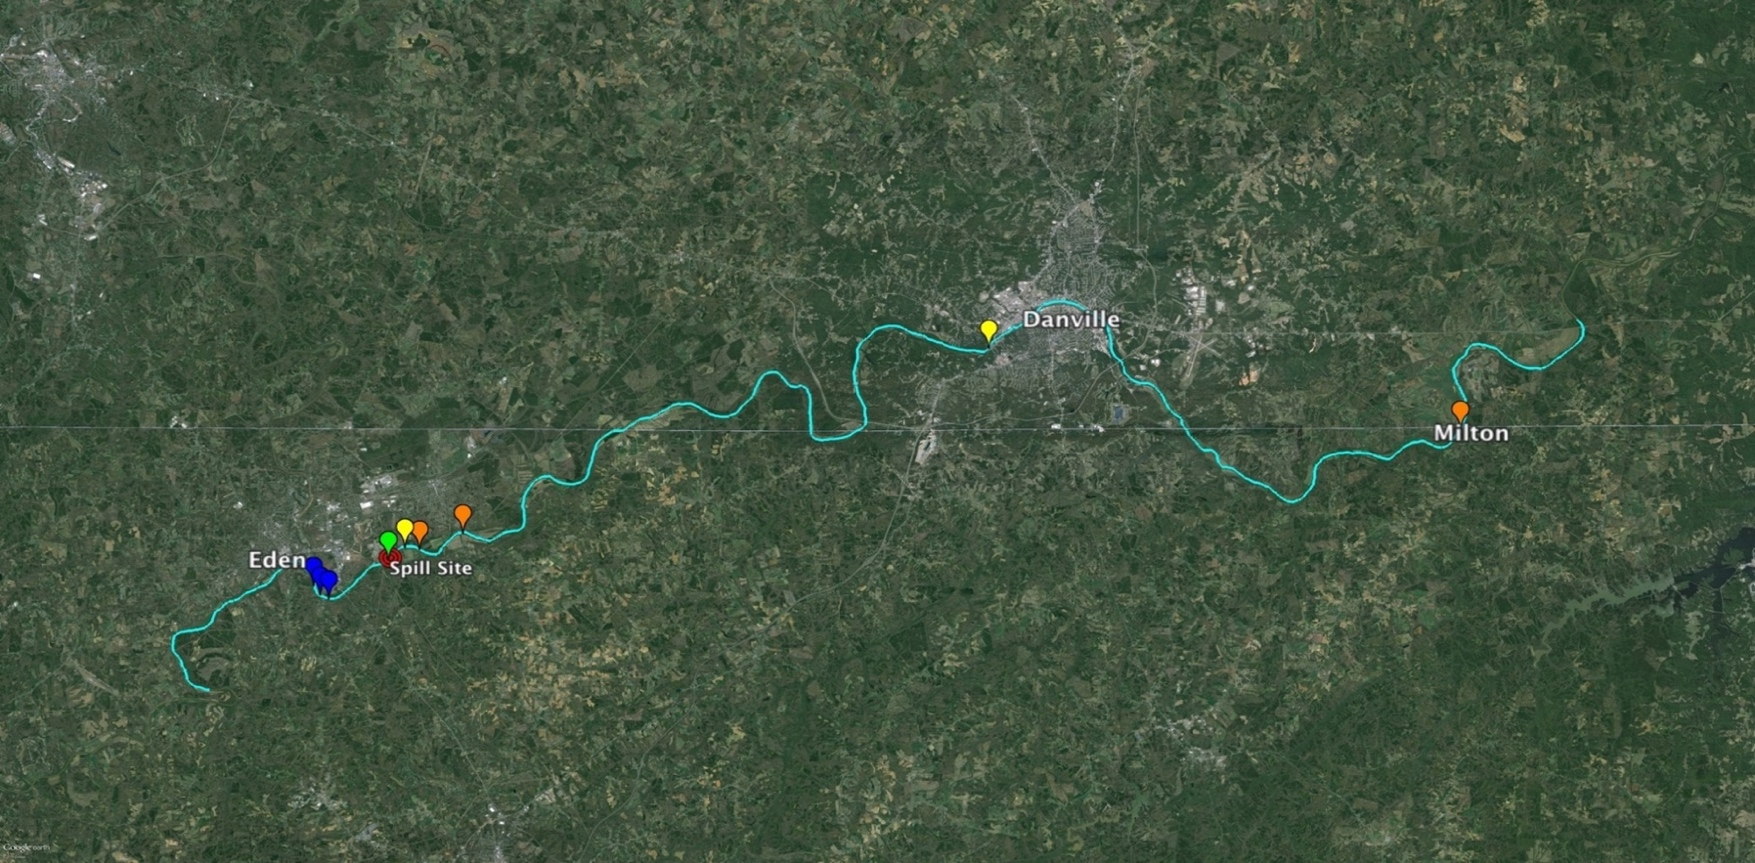
\includegraphics[width=375pt]{figure/map}
\titlecaption{Google Earth Image of Dan River and Sampling Locations}{Google Earth Image of Dan River and Sampling Locations. Markers indicate sampling sites: Blue, upstream of spill site; Green, leaching site; Yellow, downstream dredged locations; Orange, downstream not dredged.}
\label{fig:map}
\end{figure}

\FloatBarrier
Each site was accessed by boat, where sediment from the riverbank and channel was collected. Riverbank sediment cores were collected in triplicate using a piston-style coring device. Channel samples were collected using a small dredge. Sediment cores were sectioned by depth and individual segments homogenized according to one of three sampling schemes to reduce the total number of samples to be assayed (Table \ref{tab:scheme}). 0.25 \(\mathrm{cm^3}\) samples were preserved in CTAB (cetyltrimethylammonium bromide) for DNA extraction. Channel sediment was homogenized then 0.25 \(\mathrm{cm^3}\) was preserved in CTAB.
This field study was constrained by access with few boat ramps, and two dams. Frequent high water levels also provided a logistical obstacle for repeated field sampling. Additionally, the leaching site was accessed after permission from Duke Energy using their onsite boat ramp.

\begin{table}[htbp]
  \titlecaption{Sampling Locations.}{}\label{tab:sites}
  \centering
  \begin{tabular}{>{\centering\arraybackslash}p{1.5cm}>{\centering\arraybackslash}p{1.5cm}c>{\centering\arraybackslash}p{1.5cm}>{\centering\arraybackslash}p{1.5cm}>{\centering\arraybackslash}p{1.5cm}}
  \toprule
  Site ID & Distance from Spill (km) & Longitude and Latitude & Sampling Scheme & Shore Samples (n) & Channel Samples (n)\\
  \midrule
  U-03 & 3.6 & N 36 28.605, W 079 45.018 & B & 6 & 1\\
  U-02 & 2.7 & N 36 28.261, W 079 44.598 & C & 4 & 1\\
  U-01 & 1.6 & N 36 28.574, W 079 43.989 & A & 2 & 1\\
  L-01 & 0.0 & N 36 29.188, W 079 43.025 & B & 6 & 0\\
  D-01 & 0.3 & N 36 29.471, W 079 42.722 & B & 6 & 1\\
  D-02 & 1.0 & N 36 29.895, W 079 40.836 & C & 4 & 1\\
  D-03 & 4.3 & N 36 34.716, W 079 29.596 & C & 5 & 1\\
  D-04 & 36.6 & N 36 34.514, W 079 27.024 & B & 6 & 1\\
  D-05 & 38.0 & N 36 34.448, W 079 26.211 & A & 3 & 1\\
  D-06 & 64.7 & N 36 32.279, W 079 13.038 & A & 2 & 1\\
  \bottomrule
  \end{tabular}
\end{table}

\begin{table}[htbp]
  \titlecaption{Sediment Sampling Schemes.}{}\label{tab:scheme}
  \centering
  \begin{tabular}{c>{\centering\arraybackslash}p{10cm}c}
  \toprule
  Scheme & Description & Total (n)\\
  \midrule
  A & Triplicate cores segmented at 8 cm and 16 cm, segments pooled & 2\\
  B & Triplicate cores segmented at 8 cm and 16 cm, each core sampled & 6\\
  C & Triplicate sediment cores pooled at 0-4 cm, 4-8 cm, 8-12 cm, 12-16 cm & 4\\
  \bottomrule
  \end{tabular}
\vspace{24pt}
\end{table}

\FloatBarrier
\subsection{DNA Extraction and qPCR}\label{dna-extraction-and-qpcr}
A CTAB extraction of DNA was performed using standard protocol for each sample (Stewart and Via, 1993). The DNA extracted was quantified and subsequently diluted to a standard concentration of 5 ng/µL in TE (Tris-EDTA) buffer pH 8.0 and stored at 4ºC. Extracted DNA quantity and purity were determined from 2 µL subsamples of each extraction using Thermo Scientific Nanodrop Spectrophotometer based on the 260/280 nm wavelength ratio.

An Applied Biosystems StepOne real-time PCR System was utilized to detect, amplify, and quantify target DNA and representative taxa to meet the objective. Primers were chosen from literature targeting a general metabolic category. These include generic primers to the \emph{hgcA} gene, a sulfate reducing gene, \emph{dsr}, and the 16S rDNA of iron reducing bacteria. (Geets \emph{et al.} (2006);Schaefer \emph{et al.} (2014);Wagner \emph{et al.} (1998);Daly \emph{et al.} (2000), Table \ref{tab:primers}). Each reaction contained the following: 10 µL of Power Sybr® Green PCR master mix, 1 µL of forward primer (10 µM), 1 µL of reverse primer (10 µM), 8 µL of sterile deionized water, and 1 µL of extracted DNA (5 ng/µL). Three negative control reactions, samples repeated in triplicate, and positive standard controls serially diluted in triplicate, were ran in each 48 well plate. Extracted DNA from a pure culture of \emph{Desulfovibrio africanus} (ATCC 19997), an isolate known to contain the \emph{hgcA} gene was used as a standard for the \emph{hgcA} and SRB targets (Christensen \emph{et al.}, 2016). Genomic DNA extracted from \emph{Geobacter metallireducens} (ATCC 53774) served as the positive control and standard for FeRB primers (Christensen \emph{et al.}, 2016). The real-time qPCR run method consisted of a holding stage for 5 minutes at 95ºC, followed by 40 cycles of 15 seconds at 95ºC, 1 minute at 57ºC, one minute at 72ºC, and a 15-second data collection at 80ºC, followed by a melt curve analysis beginning at 95ºC, dropping to 60ºC and increasing at 0.3ºC every second until it reaches 95ºC. The relative abundance of targets was computed by the StepOne software using the standard curve. The melt curve was examined to ensure amplicon specificity.

The target abundance was normalized to the volume of extracted sediment as well as to organic matter. The amount of organic matter present in each sample was determined by ash free dry mass (AFDM). Each sample was dried at 60ºC for 48 hours, then combusted in a muffle furnace at 500ºC for 2 hours. Samples were weighed before and after combustion to calculate the AFDM.

\begin{table}[htbp]
  \titlecaption{ Primers Used in this Study}{}\label{tab:primers}
  \centering
  \begin{tabular}{llll}
  \toprule
  Target & Primer Name & Primer Sequence 5’-3’ & Reference\\
  \midrule
  \em{hgcA} & hgcA4R & CGCATYTCCTTYTYBACNCC & Liu \emph{et al.,} 2014\\
   & hgcA4F & GGNRTYAAYRTCTGGTGYGC & \\
  FeRB & Geo-R & TACCCGCTACACCTAGT & Medihala \emph{et al.,} 2012\\
   & Geo-F & AGGAAGCAACGGCTAACTCC & \\
  SRB & DSV230R & GRGYCYGCGTYYCATTAGC & Daly \emph{et al.,} 2000\\
   & DSV838F & SYCCGRCAYCTAGYRTYCATC & \\
  \bottomrule
  \end{tabular}
  \vspace{12pt}
\end{table}

\subsection{Statistical Analysis}\label{statistical-analysis}
Statistical analyses included nonparametric tests for significance to determine the overall effect of sampling location on the abundance of target per sample. To determine whether abundance of the targets vary in the shore sediment based on the distance from the spill site, the data was first tested for normality with the Shapiro-Wilk test of normality. The data did not follow a Gaussian distribution, therefore, the data were transformed (LN(x +1)), but still failed the test for normality. Samples were binned according to location irrespective of depth due to limited replication of depths, and evaluated with nonparametric tests. For each target, a Kruskall-Wallis test was performed to assess whether a difference in target abundance exists between sites. Where a significant difference was observed, a Wilcoxon Rank Sum test was performed to determine differences between sampling locations of interest. We hypothesized an increase in DNA abundance with proximity to the spill site, therefore, pairwise comparisons were assessed between Site ID D-01 and all others, as well as L-01 to all others. These tests were then repeated with the data normalized to the mass of sediment and to the amount of organic matter present in each sample.

Due to the lack of replication of river channel samples, the samples collected from the river channel bottom were binned into upstream and downstream groups. A Wilcoxon Rank Sum test was used to determine significance. All analyses were conducted using R (R Core Team, 2019).

\section{Results}\label{results}
\subsection{Shore Sediment Samples}\label{shore-sediment-samples}

The Kruskall-Wallis test revealed a significant difference between the abundance of amplified DNA and sampling locations for each of the three qPCR targets assessed (Kruskall-Wallis p-value \textless0.05). Each of the targets amplified from the D-01 sampling site, the first sampling site downstream (0.3 km) from the spill site, was detected at a higher abundance compared to at least one of the sites downstream and upstream (Figures \ref{fig:hgcaomp} - \ref{fig:srbomp}, Table \ref{tab:compare}). However, D-01 was not the location with the highest overall abundance of these targets. The sampling location U-03, the farthest upstream location, 3.6 km upstream of the spill, and 0.5 km downstream from the Smith River confluence, showed the highest values for each of the targets tested (Figures \ref{fig:hgcaomp} - \ref{fig:srbomp}, Table \ref{tab:compareU}).

\begin{figure}[htbp]
    \includegraphics[width=400pt]{figure/hgcaomp}
    \titlecaption{\textit{hgcA} Abundance Normalized to Organic Matter at Each Sampling Location}{\textit{hgcA} Abundance Normalized to Organic Matter at Each Sampling Location. Asterisks signify difference between the reference, D-01 using the Wilcoxon Rank Sum test. * : p <= 0.05, ** : p <= 0.01}\label{fig:hgcaomp}
\end{figure}
\clearpage
\begin{figure}
  \includegraphics[width=400pt]{figure/ferbomp}
   \titlecaption{FeRB Abundance Normalized to Organic Matter at Each Sampling Location}{FeRB Abundance Normalized to Organic Matter at Each Sampling Location. Asterisks signify difference between the reference, D-01 using the Wilcoxon Rank Sum test. * : p <= 0.05, ** : p <= 0.01}\label{fig:ferbomp}
\end{figure}
\clearpage
\begin{figure}
  \includegraphics[width=400pt]{figure/srbomp}
   \titlecaption{SRB Abundance Normalized to Organic Matter at Each Sampling Location}{SRB Abundance Normalized to Organic Matter at Each Sampling Location. Asterisks signify difference between the reference, D-01 using the Wilcoxon Rank Sum test. * : p <= 0.05, ** : p <= 0.01}\label{fig:srbomp}
\end{figure}
\clearpage
\begin{table}[htbp]
  \centering
  \titlecaption{Comparisons of Each Sampling Location to the Location Directly Downstream of the Spill}{Comparisons of Each Sampling Location to the Location Directly Downstream of the Spill. Wilcoxon Rank Sum Test, ns: not significant, * : p <= 0.05, ** : p <= 0.01}\label{tab:compare}
    \begin{tabular}{llll}
  \toprule
  Location & \textit{hgcA} & FeRB & SRB\\
  \midrule
  U-03 & ns & ** & ns\\
  U-02 & ** & ns & *\\
  U-01 & ns & ns & ns\\
  L-01 & ns & ns & ns\\
  D-02 & ** & ** & **\\
  D-03 & ns & * & *\\
  D-04 & ns & ns & ns\\
  D-05 & * & * & *\\
  D-06 & ns & ns & ns\\
  \bottomrule
  \end{tabular}
  \vspace{-12pt}
\end{table}

\begin{table}[htbp]
  \centering
  \titlecaption{Comparisons of Each Sampling Location to the Furthest Upstream Location}{Comparisons of Each Sampling Location to the Furthest Upstream Location. Wilcoxon Rank Sum Test, ns: not significant, * : p <= 0.05, ** : p <= 0.01}\label{tab:compareU}
  \begin{tabular}{llll}
  \toprule
  Location & \textit{hgcA} & FeRB & SRB\\
  \midrule
  U-03 & ns & ** & ns\\
  U-02 & ** & ns & *\\
  U-01 & ns & ns & ns\\
  L-01 & ns & ns & ns\\
  D-02 & ** & ** & **\\
  D-03 & ns & * & *\\
  D-04 & ns & ns & ns\\
  D-05 & * & * & *\\
  D-06 & ns & ns & ns\\
  \bottomrule
  \end{tabular}
  \vspace{18pt}
\end{table}

Additionally, the leaching site, L-01 is not significantly different from the D-01 location. When comparing the leaching site to all others, targets abundance is slightly higher than most of the other sampling locations. This pattern is similar to the D-01 comparisons, but overall, less pairs are significantly different (Table \ref{tab:compareL}). The same pattern was observed between the data normalized to the mass of sediment in each sample as well as the amount of organic matter present.

\begin{table}[htbp]
  \centering
  \titlecaption{Comparisons of Each Sampling Location to the Leaching Site Location}{Comparisons of Each Sampling Location to the Leaching Site Location. Wilcoxon Rank Sum Test, ns: not significant, * : p <= 0.05, ** : p <= 0.01}\label{tab:compareL}
  \begin{tabular}{llll}
  \toprule
  Location & \textit{hgcA} & FeRB & SRB\\
  \midrule
U-03 & ns & ** & ns\\
U-02 & ** & ns & *\\
U-01 & ns & ns & ns\\
L-01 & ns & ns & ns\\
D-02 & ** & ** & **\\
D-03 & ns & * & *\\
D-04 & ns & ns & ns\\
D-05 & * & * & *\\
D-06 & ns & ns & ns\\
  \bottomrule
  \end{tabular}
  \vspace{18pt}
\end{table}

Within this study, replication of core depth was limited, therefore, the interaction between the depth of samples was not evaluated. However, a scatterplot of the data did not show any clear patterns indicating a depth interaction, but the effect is inconclusive (Figure \ref{fig:depth}).

\begin{figure}[htbp]
\includegraphics[width=400pt]{figure/depth}
   \titlecaption{Target DNA Concentration at Each Depth}{Target DNA Concentration at Each Depth.}
   \label{fig:depth}
   \vspace{18pt}
\end{figure}


\subsection{River Channel Samples}\label{river-channel-samples}

The samples collected in the river channel were limited by one sample at each site. To assess significance, samples were binned according to upstream and downstream. For each of the targets tested, there is no significant difference between the groups (Figure \ref{fig:channel}).

\begin{figure}[htbp]
  \includegraphics[width=400pt]{figure/channel}
  \titlecaption{River Channel Abundance at Sampling Sites Upstream and Downstream Normalized to Organic Matter}{River Channel Abundance at Sampling Sites Upstream and Downstream Normalized to Organic Matter.}\label{fig:channel}
  \vspace{12pt}
\end{figure}


\section{Discussion}\label{discussion}
\addtocontents{toc}{\vspace{12pt}}
All primers tested exhibited similar patterns of significance and abundance per location. The abundance of targets detected at the sampling location 0.3 km downstream of the spill site, D-01, is higher than some locations upstream and downstream. However, the highest abundance of these three targets was found at the furthest upstream site of all locations. Also, the leaching site, L-01, exhibited higher target signal over some locations. This may signify that there could be stimulation of microbial growth, but assessment of DNA abundance does not inform methylation activity. Mercury methylation is dependent on environmental factors, where substrates such as inorganic mercury, sulfate, and organic matter must be unbound and freely available for uptake under anoxic conditions.

The results from this microbial study are inconclusive. We attempted to better define the mercury methylating potential of the microbial community using primers from (Christensen \emph{et al.}, 2016), but experienced technical difficulties and were not able to successfully use them. Hg contamination within the sediment may still be possible, and our methods of sampling sediment may not have been robust to the variable and ``hotspot'' nature of the coal ash deposition and dispersal into the river sediments. It is plausible that 1.5 years after the spill event, the coal ash is buried in the sediment, the substrates may not be available for uptake, or the coal ash has been transported further downstream than our furthest downstream location.

\chapter{IDENTIFICATION AND CHARACTERIZATION OF HEAVY METAL TOLERANCE OF BACTERIA ISOLATED FROM COAL ASH}\label{metal}
\section{Introduction}\label{introduction-1}

Coal ash is a waste product generated from coal-fired power plants. These power plants are located near water sources to meet water demands during the electricity generation process. The ash and other waste products are discharged as a slurry into a settling pond, after the combustion process (Connors, 2015). To prevent overflow the pond is maintained by pumping surface water into the nearby waters, usually a river. In North Carolina, 14 such coal ash ponds are maintained by Duke Energy. Unlined and uncapped coal ash waste ponds therefore have the potential for leaching contaminants into the groundwater or spilling into nearby waterways possibly polluting drinking water and/or disrupting aquatic ecological communities (Otter \emph{et al.}, 2012; Ruhl \emph{et al.}, 2009).

On February 2, 2014, a coal ash pond located at the retired Dan River Steam Station near Eden, NC expelled approximately 39,000 tons of coal ash slurry into the Dan River of North Carolina due to an underground pipe collapse (NC DEQ, 2014). The ash was dispersed along the river bottom between the spill site and the Kerr Reservoir, approximately 120 km downstream (Hesterberg \emph{et al.}, 2014). Dredging operations conducted by Duke Energy at Town Creek and an area upstream from the Schoolfield Dam in Danville, VA, removed approximately 2,500 tons of coal ash-laden sediment, but the remainder was deposited in the river bottom (Lemly, 2015).

Physical and chemical properties of coal ash are determined by the geographic location where the raw coal was mined, the type of boiler, and the operating conditions of the power plant (Jayaranjan \emph{et al.}, 2014). Most natural elements can be found in coal ash including trace elements such as arsenic, cadmium, chromium, mercury, lead, selenium, and zinc (Greely Jr. \emph{et al.}, 2014; Jayaranjan \emph{et al.}, 2014). Coal ash is wholly comprised of multiple waste products with differing chemical properties including fly ash, bottom ash, and byproducts of pollution mitigation processes, such as scrubber systems. Fly ash is composed mainly of oxides such as, \(\mathrm{SiO_2}\), \(\mathrm{Al_2O}\), \(\mathrm{Fe_2O}\). Bottom ash consists of silicate, carbonate, aluminate, ferrous materials and high concentrations of several heavy metals and metalloids (Kisku \emph{et al.}, 2018).

Heavy metals are characterized by a density greater than 5 g/\(\mathrm{cm^3}\), mostly transition elements, and play an important role as trace elements in biochemical reactions. These heavy metals, due to an incompletely filled d orbital, allow the cations to form complex compounds with the potential to be redox reactive. Heavy metal ions form unspecific complex compounds in living cells, leading to toxic effects. For example, \(\mathrm{Hg^{2+}}\), \(\mathrm{Cd^{2+}}\), and \(\mathrm{Ag^{+}}\) form strong toxic complexes that are not conducive to any physiological function. Trace metals such as \(\mathrm{Zn^{2+}}\), \(\mathrm{Ni^{2+}}\), and \(\mathrm{Cu^{2+}}\) are required for some biological functions but they are toxic at high concentrations Hesterberg \emph{et al.} (2014). Therefore, the intracellular concentration of heavy metals must be controlled, and organisms have adapted heavy metal resistance strategies (Binkley and Simpson, 2003; Poulain and Barkay, 2013).

Through the process of coal combustion, the coal ash is rendered sterile. Therefore, inoculation of coal ash in waste ponds occurs by natural processes including atmospheric deposition through rainfall and windblown particulates. Opportunistic microorganisms may be adapted, or may be able to adapt, to the high concentration of heavy metals through resistance or metal detoxification. Perturbations such as coal ash spills result in altered environments in receiving waters, which microbes may adapt to and subsequently mobilize coal ash constituents into food webs. Knowledge of the microbial community structure and distribution is important to estimate the extent of biological mobility of these pollutants. Further, organisms which exhibit metal tolerance may warrant further investigation into their potential for bioremediation (Keshri \emph{et al.}, 2014; Naik and Dubey, 2013; Pepi \emph{et al.}, 2011; Raja and Omine, 2012).

The objective of this study was to determine if a microbial community is viable and present in coal ash ponds, and if present, identify the taxa and assess the metal tolerance of isolated organisms. Klubek \emph{et al.}, 1992 analyzed the microbial community of coal ash ponds, but this study did not identified groups of metabolic capabilities. Roychowdhury \emph{et al.} 2018, isolated 10 bacteria representing three genera from wheathered fly ash pond samples. Raja and Omine 2013, identified boron tolerant isolates from a fly ash dumping site, and Stepanauskas \emph{et al.} 2005, evaluated the metal tolerance of microbial communities of intake and discharge of coal ash ponds. In a preliminary PCR analysis, a small amount of DNA was present in a coal ash sample from the Dan River Steam Station coal ash pond, but we were not able to amplify SSU rDNA from bacteria with universal prokaryotic primers, possibly due to contaminants present in the sample or low concentrations of bacterial DNA. Therefore, in this study, we increased the abundance of microbes and their DNA by culturing and isolating bacteria from samples of coal ash, to ensure adequate amounts of DNA for analyses.


\subsection{Objectives and Hypotheses}\label{objectives-and-hypotheses}
\textbf{Objective 1: To identify isolated bacteria using qPCR amplification and rDNA sequencing. I seek to identify these taxa using qPCR amplification and rDNA sequencing to compare to the GenBank database.}

\emph{I hypothesize novel organisms may be discovered which may have unique metal tolerance capabilities that may be useful for bioremediation.}

\textbf{Objective 2: To determine the metal tolerance of bacteria isolated from coal ash collected from the Dan River impoundment site.}

\emph{I hypothesize that microbial growth of bacterial isolates from pure coal ash collected at the Dan River Steam Station impoundment pond will be tolerant to heavy metals.}


\section{Methods}\label{methods-1}
\subsection{Pure Culture Isolation from Coal Ash}\label{pure-culture-isolation-from-coal-ash}

Samples of coal ash provided by our collaborator, Brian Williams of the Dan River Basin Association, were taken directly from a coal ash retention pond at the retired Dan River Steam Station near Eden, NC. To culture organisms, aliquots (0.5 g) of coal ash from the pond were added to six 50 mL conical tubes. 40 mL of filter sterilized (0.22 µm pore) Dan River water was added to three tubes and filter sterilized Dan River water supplemented with 10\% nutrient broth to the other three tubes. Additionally, filter sterilized Dan River water alone was evaluated in triplicate to serve as a sterility control. Tubes were incubated at ambient room temperature for 48 hours without agitation. 1 mL aliquots were then transferred from each culture and spread on 50\% nutrient agar plates for isolation. Morphologically unique colonies identified on spread plates were isolated and pure cultures maintained on 50\% nutrient agar slants for heavy metal tolerance experimentation. 

\subsection{Heavy Metal Tolerance Characterization}\label{heavy-metal-tolerance-characterization}

Optical density (OD) at 580 nm, of liquid broth culture was assessed as a proxy for growth of organisms, since growth is related to the increase in turbidity of a bacterial culture. Metals tested include, arsenic, cadmium, chromium, mercury, lead, selenium and zinc. Stock concentrations of \(\mathrm{Na_2HAsO_4}\), \(\mathrm{CdCl_2}\), \(\mathrm{CrCl_3}\), \(\mathrm{HgCl_2}\), \(\mathrm{PbCl_2}\), \(\mathrm{Na_2SeO_3}\), and \(\mathrm{ZnCl_2}\) were serially diluted to span several orders of magnitude greater and less than natural environmental concentrations reported in the literature for each metal, resulting in five concentration levels per metal (Table \ref{tab:metals}).

\begin{table}[htbp]
\titlecaption{Final Concentrations of Metal in Broth (nM)}{Final Concentrations of Metal in Fermentation Broth (nM).}\label{tab:metals}
\centering
\begin{tabular}{cccccccc}
\toprule
Factor & As & Cd & Cr & Hg & Pb & Se & Zn\\
\midrule
0 & 0 & 0 & 0 & 0 & 0 & 0 & 0\\ 
1 & 0.000135 & 0.008896 & 0.001923 & 0.004985 & 0.04826 & 0.1266 & 0.0153\\
2 & 0.00135 & 0.08896 & 0.01923 & 0.04985 & 0.4826 & 1.266 & 0.153\\
3 & 0.0135 & 0.8896 & 0.1923 & 0.4985 & 4.826 & 12.66 & 1.53\\
4 & 0.135 & 8.896 & 1.923 & 4.985 & 48.26 & 126.6 & 15.3\\
5 & 1.35 & 88.96 & 19.23 & 49.85 & 482.6 & 1266 & 153\\
\bottomrule
\end{tabular}
\vspace{18pt}
\end{table}

Metal stocks were prepared by dissolving each metal salt in sterile reverse osmosis deionized (RO/DI) water and subsequently diluted. To ensure a viable culture inoculum, sufficient volume of cells, and standardization for experimentation, each unique isolate was incubated in a 50\% nutrient broth culture in a shaking water bath at 25ºC overnight until an optical density of at least 0.7 at 580 nm was observed. For each metal-isolate experiment, 100 µL of 0.7 OD\textasciitilde580 nm\textasciitilde{} inoculum was added to 2.4 mL of 50\% nutrient broth amended with 100 µL each concentration of metal in triplicate. For the control, 100 µL of RO/DI water was substituted for the metal spike in triplicate. Growth patterns were measured by absorbance at 580 nm, and recorded at ten time points, approximately 0, 1, 2, 4, 8, 16, 24, 30, 36, and 48 hours post inoculation.


\subsection{Isolate Identification and Phylogenetic Analysis}\label{isolate-identification-and-phylogenetic-analysis}

Isolates were grown in 50\% nutrient broth then pelleted by centrifugation. The pellet was resuspended in CTAB buffer. DNA was extracted and purified using the CTAB method (Stewart and Via, 1993), then amplified with universal 16S primers (Bruce \emph{et al.}, 1992; Edwards \emph{et al.}, 1989). PCR products were then purified and commercially sequenced. Sequence chromatogram data was evaluated and edited manually to optimize the sequence. The FASTA files of sequences were imported into Molecular Evolutionary Genetics Analysis version 7.0 (MEGA7) (Kumar \emph{et al.}, 2016). Sequences were aligned using MUSCLE and manual adjustments (Edgar, 2004). The resulting aligned sequences were then subjected to phylogenetic tree analysis using MEGA7. The maximum likelihood tree was computed using MEGA7 using the Jukes-Cantor model (Jukes and Cantor, 1969). The bootstrap consensus tree was inferred from 1000 replicates. Initial trees with a greater log likelihood value were calculated by applying Neighbor-Join and BioNJ algorithms to a matrix of pairwise distances estimated using the Maximum Composite Likelihood approach. To identify the genus of each isolate, the sequences were compared to the NCBI GenBank database with BLASTn (Nucleotide Basic Local Alignment Search Tool). Genus calls were made with similarities greater than 97\% (Clark \emph{et al.}, 2016).

\subsection{Statistical Analyses}\label{statistical-analyses}

To characterize the heavy metal tolerance of isolates in liquid broth culture, the carrying capacity and growth rate of each isolate-metal experiment was modeled with a Gompertz sigmoidal function (Zwietering \emph{et al.}, 1990). Significant differences of growth rate and carrying capacity within each experiment were determined using the Kruskall-Wallis one-way analysis of variance test (p-value \textless{} 0.05). Experiments were excluded from analysis where no growth was observed in the control. Isolates were deemed metal tolerant at the concentrations tested if no significant difference between carrying capacity or growth rate was observed between concentrations.

\section{Results}\label{results-1}
\subsection{Phylogenetic Analysis}\label{phylogenetic-analysis}

A total of 31 microorganisms were isolated from the coal ash sample and sequenced. Sequences were aligned and a phylogenetic tree was constructed (Figure \ref{fig:tree}). Sequences were predominantly identified as \emph{Bacillus} or \emph{Arthrobacter} spp. One isolate, DR 76, was not identified in GenBank with the BLASTn search. 

\begin{figure}[htbp]
  \centering
  \includegraphics{figure/tree7}
  \titlecaption{Phylogenetic Analysis of Isolates Cultured from Coal Ash Amended Media}{Phylogenetic Analysis of Isolates Cultured from Coal Ash Amended Media.}\label{fig:tree}
\end{figure}
\FloatBarrier
\subsection{Metal Tolerance Assays}\label{metal-tolerance-assays}
We tested metal tolerance of 14 isolates. The isolates were challenged against seven metals, resulting in a total of 94 trials. Isolates generally grew well. Figures \ref{fig:dr13} - \ref{fig:dr52} are exemplary of typical growth responses. Figure \ref{fig:dr13} is representative of similar growth response among differing metal concentrations. Carrying capacity is significantly different between metal concentrations of Cd and Zn, and growth rates are different with As and Zn. Figure \ref{fig:dr32} showed a varied response where carrying capacity is significantly different between metal concentrations of Cd and Se, but no difference is observed when testing maximal growth rates. Figure \ref{fig:dr52}, Se is an example of no growth. When evaluating the growth of DR 52 challenged by the other metals, the carrying capacity is significantly different between metal concentrations of Cd, and growth rates are different with As, Cd, and Hg (Kruskall-Wallis test p-value < 0.05). 

When evaluating carrying capacity, 70 trials were not different from the control, that is, they were metal tolerant (Kruskall-Wallis test p-value \textgreater0.05, Table \ref{tab:kpvalue}). Evaluation of maximal growth rate produced 71 isolate-metal trials that were tolerant (Table \ref{tab:muvalue}). Metal intolerance (i.e. reduced growth rate or lower carrying capacity) was found in 64\% of the isolates tested with Cd and 72\% are susceptible to Se. The other metals tested (As, Cr, Hg, Pb, and Zn) resulted in much less susceptibility, ranging from 1-3 susceptible isolates.

High concentrations of Cd had an effect on most of the isolates tested. Of the five isolates that were tolerant of Cd, one is \emph{Arthrobacter}, although not all \emph{Arthrobacter} were tolerant of Cd. \emph{Bacillus} spp. are genomically diverse, ubiquitous endospore-formers are highly resistant to stressors (Earl \emph{et al.}, 2008). Two \emph{Bacillus} spp. were subjected to metal tolerance assays. The \emph{Bacillus} spp. DR52 and DRp51 exhibited the same metal tolerance characterization; tolerant to all except Cd and Se.

\begin{figure}[t]
  \centering
  \includegraphics[width=400pt]{figure/dr13plot}
  \titlecaption{Growth of Isolate DR13}{Growth of Isolate DR13. Lines connect means of three replicates, colors represent concentration levels (Table 3.1). Carrying capacity is significantly different between metal concentrations of Cd and Zn.  Growth rates are different with As and Zn (Kruskall-Wallis test p-value < 0.05)}
  \label{fig:dr13}
\end{figure}

\begin{figure}[t]
  \centering
  \includegraphics[width=400pt]{figure/dr32plot}
  \titlecaption{Growth of Isolate DR3.2}{Growth of Isolate DR3.2. Lines connect means of three replicates, colors represent concentration levels (Table 3.1). Carrying capacity is significantly different between metal concentrations of Cd and Se. No difference is observed when testing maximal growth rates (Kruskall-Wallis test p-value < 0.05)}
  \label{fig:dr32}
\end{figure}

\begin{figure}[t]
  \centering
  \includegraphics[width=400pt]{figure/dr52plot}
  \titlecaption{Growth of Isolate DR52}{Growth of Isolate DR52. Lines connect means of three replicates, colors represent concentration levels (Table 3.1). Se was excluded from analysis. Carrying capacity is significantly different between metal concentrations of Cd. Growth rates are different with As, Cd, and Hg. (Kruskall-Wallis test p-value < 0.05) }
  \label{fig:dr52}
\end{figure}

\clearpage
\begin{table}[htbp]
  \titlecaption{P-values of Kruskall-Wallis Test of Carrying Capacity}{P-values of Kruskall-Wallis Test of Carrying Capacity. Bold typeface signifies p-value <0.05. NA: Not Analyzed (Data listed in Appendix)}
  \label{tab:kpvalue}
  \centering
  %\resizebox{\linewidth}{!}{
  \begin{tabular}{lllllllll}
  \toprule
  \multicolumn{1}{c}{Genus} & \multicolumn{1}{c}{Isolate} & \multicolumn{1}{c}{As} & \multicolumn{1}{c}{Cd} & \multicolumn{1}{c}{Cr} & \multicolumn{1}{c}{Hg} & \multicolumn{1}{c}{Pb} & \multicolumn{1}{c}{Se} & \multicolumn{1}{c}{Zn}\\
  \midrule
  \rowcolor{gray!6}  Not Sequenced & DR13 & 0.138 & \textbf{0.046} & 0.148 & 0.086 & 0.281 & 0.083 & \textbf{0.025}\\
  \em{Arthrobacter} & DR24 & 0.141 & \textbf{0.025} & 0.554 & 0.504 & 0.163 & NA & \textbf{0.022}\\
  \rowcolor{gray!6}  \em{Sinomonas} & DR26 & 0.482 & \textbf{0.02} & 0.612 & 0.547 & 0.134 & \textbf{0.011} & 0.067\\
  \em{Arthrobacter} & DR3.2 & 0.367 & \textbf{0.027} & 0.637 & 0.091 & 0.669 & \textbf{0.011} & 0.344\\
  \rowcolor{gray!6}  \em{Arthrobacter} & DR5 & 0.171 & 0.203 & 0.961 & 0.494 & 0.075 & 0.074 & 0.16\\
  \em{Bacillus} & DR52 & 0.364 & \textbf{0.009} & 0.691 & 0.425 & 0.066 & NA & 0.081\\
  \rowcolor{gray!6}  \em{Arthrobacter} & DR60 & \textbf{0.038} & \textbf{0.04} & 0.097 & 0.135 & 0.074 & NA & 0.164\\
  Unknown Genus & DR76 & 0.125 & 0.336 & 0.517 & NA & 0.18 & \textbf{0.014} & \textbf{0.02}\\
  \rowcolor{gray!6}  \em{Bacillus} & DRp51 & 0.116 & \textbf{0.014} & 0.54 & 0.713 & 0.787 & \textbf{0.008} & 0.193\\
  \em{Lynsinibacillus} & DRp72 & 0.173 & \textbf{0.018} & 0.096 & 0.057 & 0.43 & NA & 0.104\\
  \rowcolor{gray!6}  \em{Pelemonas} & DRp74 & 0.385 & 0.105 & \textbf{0.015} & \textbf{0.016} & 0.131 & \textbf{0.032} & 0.669\\
  Not Sequenced & NO14 & 0.243 & \textbf{0.031} & 0.297 & 0.97 & 0.822 & \textbf{0.03} & 0.741\\
  \rowcolor{gray!6}  Not Sequenced & NO17 & 0.051 & 0.067 & 0.22 & 0.329 & \textbf{0.035} & 0.054 & 0.063\\
  Not Sequenced & NO22 & NA & NA & NA & NA & NA & \textbf{0.014} & NA\\
  \bottomrule
  \end{tabular}
\end{table}

\begin{table}
  \titlecaption{P-values of Kruskall-Wallis Test of Growth Rate}{P-values of Kruskall-Wallis Test of Growth Rate. Bold typeface signifies p-value <0.05. NA: Not Analyzed (Data listed in Appendix)}
  \label{tab:muvalue}
  \centering
  %\resizebox{\linewidth}{!}{
  \begin{tabular}{lllllllll}
  \toprule
  \multicolumn{1}{c}{Genus} & \multicolumn{1}{c}{Isolate} & \multicolumn{1}{c}{As} & \multicolumn{1}{c}{Cd} & \multicolumn{1}{c}{Cr} & \multicolumn{1}{c}{Hg} & \multicolumn{1}{c}{Pb} & \multicolumn{1}{c}{Se} & \multicolumn{1}{c}{Zn}\\
  \midrule
  \rowcolor{gray!6}  Not Sequenced & DR13 & \textbf{0.042} & 0.177 & 0.445 & 0.825 & 0.251 & 0.114 & \textbf{0.021}\\
  \em{Arthrobacter} & DR24 & 0.284 & \textbf{0.026} & 0.073 & 0.183 & 0.637 & NA & \textbf{0.02}\\
  \rowcolor{gray!6}  \em{Sinomonas} & DR26 & 0.306 & 0.128 & 0.149 & 0.383 & 0.114 & \textbf{0.009} & 0.334\\
  \em{Arthrobacter} & DR3.2 & 0.206 & 0.068 & 0.171 & 0.074 & 0.213 & 0.055 & 0.083\\
  \rowcolor{gray!6}  \em{Arthrobacter} & DR5 & 0.419 & \textbf{0.036} & 0.192 & 0.637 & 0.56 & \textbf{0.012} & 0.511\\
  \em{Bacillus} & DR52 & \textbf{0.028} & \textbf{0.007} & 0.889 & \textbf{0.041} & 0.063 & NA & 0.078\\
  \rowcolor{gray!6}  \em{Arthrobacter} & DR60 & \textbf{0.028} & 0.071 & 0.054 & 0.082 & 0.141 & NA & \textbf{0.03}\\
  Unknown Genus & DR76 & 0.218 & 0.451 & 0.534 & NA & 0.399 & \textbf{0.039} & \textbf{0.028}\\
  \rowcolor{gray!6}  \em{Bacillus} & DRp51 & 0.154 & 0.138 & \textbf{0.025} & 0.439 & 0.975 & 0.136 & 0.279\\
  \em{Lynsinibacillus} & DRp72 & 0.263 & \textbf{0.035} & 0.255 & 0.158 & 0.385 & NA & 0.173\\
  \rowcolor{gray!6}  \em{Pelemonas} & DRp74 & 0.669 & 0.261 & \textbf{0.048} & \textbf{0.021} & 0.056 & 0.141 & 0.488\\
  Not Sequenced & NO14 & 0.324 & 0.086 & 0.713 & 0.9 & 0.801 & \textbf{0.014} & 0.648\\
  \rowcolor{gray!6}  Not Sequenced & NO17 & 0.174 & 0.107 & 0.68 & 0.825 & 0.112 & \textbf{0.013} & 0.286\\
  Not Sequenced & NO22 & NA & NA & NA & NA & NA & 0.05 & NA\\
  \bottomrule
  \end{tabular}
  \vspace{18pt}
\end{table}

\section{Discussion}\label{discussion-1}
\addtocontents{toc}{\vspace{12pt}}
We isolated cultures of aerobic bacteria from samples of coal ash. The coal ash isolates were predominantly identified as \emph{Arthrobacter} and \emph{Bacillus} spp. \emph{Arthrobacter} spp. are ubiquitous and have been found in common soils as well as extreme environments. Several studies have isolated bacteria from coal ash. 

Roychowdhury \emph{et al.} 2018 found 10 isolates represented by \emph{Bacillus, Micrococcus, Kytococcus, and Staphylococcus} genera. In our study we isolated 31 bacteria including 8 \emph{Bacillus} spp. but none of the other genera.  Raja and Omine 2013, using 16S rRNA sequencing and phylogenetic analysis, identified 4 genera from a fly ash dumping site, including \emph{Bacillus} and \emph{Lysinibacillus}, which we also found. They also found \emph{Microbacterium} and \emph{Ralstonia} spp. Pangayao \emph{et al.} 2018, isolated \emph{Pseudomonas} spp. from multiple coal ash ponds, which we did not find. The \emph{Arthrobacter} sp. that constituted the majority of our isolates (16 of 31), are spore-formers that are able to survive long periods of time under stressful conditions such as nutrient deficiency, temperature shifts, and toxic chemicals. They are metabolically diverse, have been utilized to biodegrade environmental pollutants, and are highly resistant to heavy metals (Mongodin \emph{et al.}, 2006). The predominance of \emph{Arthrobacter} sp. among our coal ash isolates may be due to the selective pressure of the coal ash or the isolation methods. 

One isolate could not be identified by a BLASTn search of the GenBank database, and may be an interesting organism to for further testing and characterization. Since we only studied organisms which were easily grown and maintained within the lab under room temperature conditions, likely only a very small portion of the organisms that were present in coal ash  were cultivated. More novel organisms may be discoverable using alternate culturing methods. 

Our isolates were generally metal tolerant as in previous studies. For example, Stepanauskas \emph{et al.} 2005 documented metal tolerance in bacteria from ash settling basins by flow cytometric analyses. Roychowdhury \emph{et al.} 2018 found As tolerance in isolates from wheathered pond ash samples.  Raja and Omine \emph{et al.} 2013, found boron tolerant microbes from a fly ash dumping site in Japan. All of these studies along with ours, demonstrate metal tolerance, and our assay appears useful as a screen to find interesting isolates for further study.

\chapter{CONCLUSIONS}\label{conclusions}

We found no significant evidence of increased mercury methylation potential from the coal ash spill into the Dan River. We observed similar patterns of abundance of each qPCR target among the sample locations, indicating a similar response by multiple taxonomic groups. Unexpectedly, the highest abundance among all targets was observed at a site that seems unlikely to have been contaminated with coal ash due to its distance upstream from the spill site.

The coal ash isolates were generally tolerant to the concentrations of heavy metals tested, except for cadmium and selenium. However, we did not measure the ion concentrations directly to determine if the metal was unbound and available for uptake. Alternate isolation protocols to capture a more diverse group of isolates may better improve our understanding of coal ash bacteria. 

Due to the dynamic nature of river systems, assaying for polluting spills or other perturbations is difficult. A study with  improved sampling methods may better elucidate risk of mercury-methylation and mobilization into the food webs. 

\nocite{*}

%%------------------------------------------------------------------%%
%%------------------------ Bibliography ----------------------------%%
%%------------------------------------------------------------------%%
%% Replace the myreferences with the name of your bib file.  Then you
%% can run bibtex as usual.
%%------------------------------------------------------------------%%

\bibliography{references}
%\bibliographystyle{cell}
\bibliographystyle{apa-good}
%\bibliographystyle{amsalpha}
%%------------------------------------------------------------------%%
%%------------------------- Appendices -----------------------------%%
%%------------------------------------------------------------------%%
%% If you choose not to have appendices, comment out the \appendix
%% line and the chapters below.
%%------------------------------------------------------------------%%
\appendix
\chapter{Supplemental Tables}\label{app:why}
\renewcommand{\thetable}{A.\arabic{table}}
\setcounter{table}{0}
\vspace{-12pt}
\begin{longtable}{ccccccc}
  \caption[DR 13 Gompertz Model Parameters.]{\label{tab:dr13}DR 13 Gompertz Model Parameters. Estimations of maximal growth rates and carrying capacities. factor = Metal Concentration Factor (Table 3.1), mumax = Maximal Growth Rate, K = Carrying Capacity}\\
  \toprule
  \multicolumn{1}{c}{Metal} & \multicolumn{1}{c}{factor} & \multicolumn{1}{c}{Replicate} & \multicolumn{1}{c}{y0} & \multicolumn{1}{c}{mumax} & \multicolumn{1}{c}{K} & \multicolumn{1}{c}{r2}\\
  \midrule
  \endfirsthead
  \caption[]{\label{tab:dr13}DR 13 Gompertz Model Parameters. Estimations of maximal growth rates and carrying capacities. factor = Metal Concentration Factor (Table 3.1), mumax = Maximal Growth Rate, K = Carrying Capacity \textit{(continued)}}\\
  \toprule
  \multicolumn{1}{c}{Metal} & \multicolumn{1}{c}{factor} & \multicolumn{1}{c}{Replicate} & \multicolumn{1}{c}{y0} & \multicolumn{1}{c}{mumax} & \multicolumn{1}{c}{K} & \multicolumn{1}{c}{r2}\\
  \midrule
  \endhead
  \
  \endfoot
  \bottomrule
  \endlastfoot
  \rowcolor{gray!6}  As & 0 & 1 & 0.031 & 0.064 & 0.431 & 0.997\\
  As & 0 & 2 & 0.032 & 0.065 & 0.427 & 0.994\\
  \rowcolor{gray!6}  As & 0 & 3 & 0.030 & 0.064 & 0.428 & 0.996\\
  As & 1 & 1 & 0.034 & 0.060 & 0.460 & 0.996\\
  \rowcolor{gray!6}  As & 1 & 2 & 0.034 & 0.055 & 0.477 & 0.993\\
  As & 1 & 3 & 0.032 & 0.061 & 0.459 & 0.996\\
  \rowcolor{gray!6}  As & 2 & 1 & 0.035 & 0.059 & 0.471 & 0.994\\
  As & 2 & 2 & 0.034 & 0.055 & 0.483 & 0.994\\
  \rowcolor{gray!6}  As & 2 & 3 & 0.034 & 0.061 & 0.457 & 0.995\\
  As & 3 & 1 & 0.034 & 0.062 & 0.453 & 0.994\\
  \rowcolor{gray!6}  As & 3 & 2 & 0.034 & 0.059 & 0.473 & 0.995\\
  As & 3 & 3 & 0.034 & 0.060 & 0.458 & 0.994\\
  \rowcolor{gray!6}  As & 4 & 1 & 0.036 & 0.062 & 0.482 & 0.995\\
  As & 4 & 2 & 0.035 & 0.060 & 0.449 & 0.994\\
  \rowcolor{gray!6}  As & 4 & 3 & 0.030 & 0.069 & 0.439 & 0.995\\
  As & 5 & 1 & 0.035 & 0.063 & 0.471 & 0.994\\
  \rowcolor{gray!6}  As & 5 & 2 & 0.035 & 0.063 & 0.459 & 0.994\\
  As & 5 & 3 & 0.034 & 0.066 & 0.434 & 0.994\\
  \rowcolor{gray!6}  Cd & 0 & 1 & 0.027 & 0.072 & 0.406 & 0.995\\
  Cd & 0 & 2 & 0.029 & 0.066 & 0.447 & 0.993\\
  \rowcolor{gray!6}  Cd & 0 & 3 & 0.030 & 0.060 & 0.496 & 0.993\\
  Cd & 1 & 1 & 0.028 & 0.069 & 0.431 & 0.997\\
  \rowcolor{gray!6}  Cd & 1 & 2 & 0.029 & 0.064 & 0.478 & 0.996\\
  Cd & 1 & 3 & 0.031 & 0.061 & 0.481 & 0.994\\
  \rowcolor{gray!6}  Cd & 2 & 1 & 0.031 & 0.065 & 0.450 & 0.993\\
  Cd & 2 & 2 & 0.030 & 0.065 & 0.450 & 0.995\\
  \rowcolor{gray!6}  Cd & 2 & 3 & 0.030 & 0.066 & 0.452 & 0.994\\
  Cd & 3 & 1 & 0.031 & 0.066 & 0.442 & 0.991\\
  \rowcolor{gray!6}  Cd & 3 & 2 & 0.030 & 0.067 & 0.435 & 0.994\\
  Cd & 3 & 3 & 0.033 & 0.062 & 0.453 & 0.992\\
  \rowcolor{gray!6}  Cd & 4 & 1 & 0.027 & 0.063 & 0.395 & 0.994\\
  Cd & 4 & 2 & 0.028 & 0.061 & 0.421 & 0.994\\
  \rowcolor{gray!6}  Cd & 4 & 3 & 0.030 & 0.060 & 0.422 & 0.993\\
  Cd & 5 & 1 & 0.017 & 0.062 & 0.385 & 0.905\\
  \rowcolor{gray!6}  Cd & 5 & 2 & 0.023 & 0.050 & 0.364 & 0.997\\
  Cd & 5 & 3 & 0.024 & 0.053 & 0.343 & 0.997\\
  \rowcolor{gray!6}  Cr & 0 & 1 & 0.028 & 0.063 & 0.445 & 0.995\\
  Cr & 0 & 2 & 0.033 & 0.063 & 0.439 & 0.994\\
  \rowcolor{gray!6}  Cr & 0 & 3 & 0.034 & 0.070 & 0.440 & 0.995\\
  Cr & 1 & 1 & 0.035 & 0.060 & 0.471 & 0.997\\
  \rowcolor{gray!6}  Cr & 1 & 2 & 0.033 & 0.064 & 0.434 & 0.996\\
  Cr & 1 & 3 & 0.033 & 0.063 & 0.439 & 0.996\\
  \rowcolor{gray!6}  Cr & 2 & 1 & 0.032 & 0.062 & 0.438 & 0.997\\
  Cr & 2 & 2 & 0.044 & 0.059 & 0.443 & 0.998\\
  \rowcolor{gray!6}  Cr & 2 & 3 & 0.033 & 0.065 & 0.411 & 0.994\\
  Cr & 3 & 1 & 0.033 & 0.062 & 0.433 & 0.995\\
  \rowcolor{gray!6}  Cr & 3 & 2 & 0.035 & 0.061 & 0.446 & 0.994\\
  Cr & 3 & 3 & 0.029 & 0.085 & 0.337 & 0.993\\
  \rowcolor{gray!6}  Cr & 4 & 1 & 0.032 & 0.059 & 0.461 & 0.993\\
  Cr & 4 & 2 & 0.034 & 0.062 & 0.452 & 0.994\\
  \rowcolor{gray!6}  Cr & 4 & 3 & 0.032 & 0.062 & 0.452 & 0.996\\
  Cr & 5 & 1 & 0.033 & 0.060 & 0.444 & 0.994\\
  \rowcolor{gray!6}  Cr & 5 & 2 & 0.034 & 0.061 & 0.454 & 0.995\\
  Cr & 5 & 3 & 0.034 & 0.062 & 0.446 & 0.996\\
  \rowcolor{gray!6}  Hg & 0 & 1 & 0.030 & 0.066 & 0.430 & 0.994\\
  Hg & 0 & 2 & 0.033 & 0.066 & 0.407 & 0.993\\
  \rowcolor{gray!6}  Hg & 0 & 3 & 0.030 & 0.063 & 0.429 & 0.994\\
  Hg & 1 & 1 & 0.032 & 0.068 & 0.423 & 0.995\\
  \rowcolor{gray!6}  Hg & 1 & 2 & 0.034 & 0.062 & 0.430 & 0.993\\
  Hg & 1 & 3 & 0.032 & 0.066 & 0.465 & 0.996\\
  \rowcolor{gray!6}  Hg & 2 & 1 & 0.034 & 0.064 & 0.438 & 0.995\\
  Hg & 2 & 2 & 0.033 & 0.064 & 0.438 & 0.994\\
  \rowcolor{gray!6}  Hg & 2 & 3 & 0.035 & 0.061 & 0.451 & 0.993\\
  Hg & 3 & 1 & 0.033 & 0.065 & 0.467 & 0.995\\
  \rowcolor{gray!6}  Hg & 3 & 2 & 0.035 & 0.063 & 0.458 & 0.993\\
  Hg & 3 & 3 & 0.033 & 0.064 & 0.459 & 0.994\\
  \rowcolor{gray!6}  Hg & 4 & 1 & 0.034 & 0.067 & 0.455 & 0.994\\
  Hg & 4 & 2 & 0.036 & 0.060 & 0.465 & 0.992\\
  \rowcolor{gray!6}  Hg & 4 & 3 & 0.034 & 0.064 & 0.432 & 0.993\\
  Hg & 5 & 1 & 0.032 & 0.072 & 0.434 & 0.994\\
  \rowcolor{gray!6}  Hg & 5 & 2 & 0.034 & 0.064 & 0.448 & 0.993\\
  Hg & 5 & 3 & 0.034 & 0.064 & 0.447 & 0.993\\
  \rowcolor{gray!6}  Pb & 0 & 1 & 0.030 & 0.067 & 0.435 & 0.995\\
  Pb & 0 & 2 & 0.030 & 0.064 & 0.463 & 0.995\\
  \rowcolor{gray!6}  Pb & 0 & 3 & 0.029 & 0.067 & 0.443 & 0.995\\
  Pb & 1 & 1 & 0.029 & 0.071 & 0.423 & 0.996\\
  \rowcolor{gray!6}  Pb & 1 & 2 & 0.030 & 0.069 & 0.430 & 0.995\\
  Pb & 1 & 3 & 0.032 & 0.063 & 0.474 & 0.995\\
  \rowcolor{gray!6}  Pb & 2 & 1 & 0.030 & 0.067 & 0.466 & 0.995\\
  Pb & 2 & 2 & 0.030 & 0.068 & 0.445 & 0.996\\
  \rowcolor{gray!6}  Pb & 2 & 3 & 0.024 & 0.072 & 0.500 & 0.980\\
  Pb & 3 & 1 & 0.030 & 0.067 & 0.424 & 0.995\\
  \rowcolor{gray!6}  Pb & 3 & 2 & 0.032 & 0.060 & 0.463 & 0.994\\
  Pb & 3 & 3 & 0.030 & 0.069 & 0.411 & 0.994\\
  \rowcolor{gray!6}  Pb & 4 & 1 & 0.032 & 0.063 & 0.448 & 0.993\\
  Pb & 4 & 2 & 0.031 & 0.064 & 0.425 & 0.993\\
  \rowcolor{gray!6}  Pb & 4 & 3 & 0.032 & 0.063 & 0.449 & 0.994\\
  Pb & 5 & 1 & 0.030 & 0.068 & 0.407 & 0.994\\
  \rowcolor{gray!6}  Pb & 5 & 2 & 0.031 & 0.065 & 0.428 & 0.993\\
  Pb & 5 & 3 & 0.032 & 0.066 & 0.432 & 0.994\\
  \rowcolor{gray!6}  Se & 0 & 1 & 0.007 & 0.070 & 0.360 & 0.995\\
  Se & 0 & 2 & 0.008 & 0.072 & 0.351 & 0.989\\
  \rowcolor{gray!6}  Se & 0 & 3 & 0.006 & 0.069 & 0.372 & 0.995\\
  Se & 1 & 1 & 0.008 & 0.062 & 0.391 & 0.993\\
  \rowcolor{gray!6}  Se & 1 & 2 & 0.007 & 0.067 & 0.341 & 0.992\\
  Se & 1 & 3 & 0.008 & 0.064 & 0.377 & 0.989\\
  \rowcolor{gray!6}  Se & 2 & 1 & 0.006 & 0.076 & 0.328 & 0.996\\
  Se & 2 & 2 & 0.008 & 0.055 & 0.424 & 0.995\\
  \rowcolor{gray!6}  Se & 2 & 3 & 0.008 & 0.055 & 0.476 & 0.995\\
  Se & 3 & 1 & 0.006 & 0.066 & 0.411 & 0.998\\
  \rowcolor{gray!6}  Se & 3 & 2 & 0.008 & 0.060 & 0.383 & 0.995\\
  Se & 3 & 3 & 0.009 & 0.056 & 0.421 & 0.994\\
  \rowcolor{gray!6}  Se & 4 & 1 & 0.007 & 0.062 & 0.413 & 0.995\\
  Se & 4 & 2 & 0.009 & 0.055 & 0.440 & 0.991\\
  \rowcolor{gray!6}  Se & 4 & 3 & 0.009 & 0.059 & 0.407 & 0.991\\
  Se & 5 & 1 & 0.007 & 0.049 & 0.497 & 0.991\\
  \rowcolor{gray!6}  Se & 5 & 2 & 0.005 & 0.055 & 0.433 & 0.996\\
  Se & 5 & 3 & 0.004 & 0.056 & 0.438 & 0.996\\
  \rowcolor{gray!6}  Zn & 0 & 1 & 0.032 & 0.071 & 0.416 & 0.993\\
  Zn & 0 & 2 & 0.033 & 0.066 & 0.427 & 0.992\\
  \rowcolor{gray!6}  Zn & 0 & 3 & 0.034 & 0.066 & 0.420 & 0.992\\
  Zn & 1 & 1 & 0.032 & 0.066 & 0.421 & 0.993\\
  \rowcolor{gray!6}  Zn & 1 & 2 & 0.034 & 0.063 & 0.461 & 0.992\\
  Zn & 1 & 3 & 0.034 & 0.064 & 0.429 & 0.990\\
  \rowcolor{gray!6}  Zn & 2 & 1 & 0.032 & 0.064 & 0.435 & 0.994\\
  Zn & 2 & 2 & 0.032 & 0.066 & 0.447 & 0.994\\
  \rowcolor{gray!6}  Zn & 2 & 3 & 0.032 & 0.068 & 0.432 & 0.994\\
  Zn & 3 & 1 & 0.031 & 0.067 & 0.430 & 0.994\\
  \rowcolor{gray!6}  Zn & 3 & 2 & 0.032 & 0.068 & 0.431 & 0.993\\
  Zn & 3 & 3 & 0.031 & 0.069 & 0.419 & 0.994\\
  \rowcolor{gray!6}  Zn & 4 & 1 & 0.029 & 0.071 & 0.426 & 0.995\\
  Zn & 4 & 2 & 0.031 & 0.071 & 0.412 & 0.993\\
  \rowcolor{gray!6}  Zn & 4 & 3 & 0.031 & 0.071 & 0.419 & 0.993\\
  Zn & 5 & 1 & 0.030 & 0.059 & 0.410 & 0.993\\
  \rowcolor{gray!6}  Zn & 5 & 2 & 0.028 & 0.060 & 0.389 & 0.993\\
  Zn & 5 & 3 & 0.025 & 0.064 & 0.377 & 0.994\\*
  \end{longtable}
  \clearpage
  \begin{longtable}{ccccccc}
  \caption[DR 24 Gompertz Model Parameters.]{\label{tab:dr24}DR 24 Gompertz Model Parameters. Estimations of maximal growth rates and carrying capacities. factor = Metal Concentration Factor (Table 3.1), mumax = Maximal Growth Rate, K = Carrying Capacity}\\
  \toprule
  \multicolumn{1}{c}{Metal} & \multicolumn{1}{c}{factor} & \multicolumn{1}{c}{Replicate} & \multicolumn{1}{c}{y0} & \multicolumn{1}{c}{mumax} & \multicolumn{1}{c}{K} & \multicolumn{1}{c}{r2}\\
  \midrule
  \endfirsthead
  \caption[]{\label{tab:dr24}DR 24 Gompertz Model Parameters. Estimations of maximal growth rates and carrying capacities. factor = Metal Concentration Factor (Table 3.1), mumax = Maximal Growth Rate, K = Carrying Capacity \textit{(continued)}}\\
  \toprule
  \multicolumn{1}{c}{Metal} & \multicolumn{1}{c}{factor} & \multicolumn{1}{c}{Replicate} & \multicolumn{1}{c}{y0} & \multicolumn{1}{c}{mumax} & \multicolumn{1}{c}{K} & \multicolumn{1}{c}{r2}\\
  \midrule
  \endhead
  \
  \endfoot
  \bottomrule
  \endlastfoot
  \rowcolor{gray!6}  As & 0 & 1 & 0.032 & 0.103 & 0.312 & 0.985\\
  As & 0 & 2 & 0.030 & 0.092 & 0.269 & 0.989\\
  \rowcolor{gray!6}  As & 0 & 3 & 0.030 & 0.098 & 0.334 & 0.988\\
  As & 1 & 1 & 0.028 & 0.101 & 0.272 & 0.984\\
  \rowcolor{gray!6}  As & 1 & 2 & 0.032 & 0.087 & 0.286 & 0.989\\
  As & 1 & 3 & 0.032 & 0.087 & 0.283 & 0.990\\
  \rowcolor{gray!6}  As & 2 & 1 & 0.033 & 0.087 & 0.263 & 0.944\\
  As & 2 & 2 & 0.030 & 0.090 & 0.276 & 0.990\\
  \rowcolor{gray!6}  As & 2 & 3 & 0.031 & 0.091 & 0.280 & 0.989\\
  As & 3 & 1 & 0.028 & 0.100 & 0.268 & 0.989\\
  \rowcolor{gray!6}  As & 3 & 2 & 0.031 & 0.091 & 0.259 & 0.952\\
  As & 3 & 3 & 0.030 & 0.090 & 0.284 & 0.989\\
  \rowcolor{gray!6}  As & 4 & 1 & 0.030 & 0.097 & 0.281 & 0.992\\
  As & 4 & 2 & 0.034 & 0.084 & 0.311 & 0.986\\
  \rowcolor{gray!6}  As & 4 & 3 & 0.031 & 0.092 & 0.288 & 0.989\\
  As & 5 & 1 & 0.028 & 0.102 & 0.288 & 0.989\\
  \rowcolor{gray!6}  As & 5 & 2 & 0.029 & 0.092 & 0.286 & 0.985\\
  As & 5 & 3 & 0.030 & 0.097 & 0.287 & 0.988\\
  \rowcolor{gray!6}  Cd & 0 & 1 & 0.032 & 0.096 & 0.277 & 0.995\\
  Cd & 0 & 2 & 0.030 & 0.093 & 0.282 & 0.990\\
  \rowcolor{gray!6}  Cd & 0 & 3 & 0.030 & 0.094 & 0.269 & 0.983\\
  Cd & 1 & 1 & 0.031 & 0.089 & 0.286 & 0.988\\
  \rowcolor{gray!6}  Cd & 1 & 2 & 0.030 & 0.088 & 0.286 & 0.987\\
  Cd & 1 & 3 & 0.029 & 0.093 & 0.274 & 0.989\\
  \rowcolor{gray!6}  Cd & 2 & 1 & 0.031 & 0.092 & 0.286 & 0.988\\
  Cd & 2 & 2 & 0.030 & 0.091 & 0.279 & 0.988\\
  \rowcolor{gray!6}  Cd & 2 & 3 & 0.029 & 0.092 & 0.284 & 0.990\\
  Cd & 3 & 1 & 0.029 & 0.094 & 0.288 & 0.990\\
  \rowcolor{gray!6}  Cd & 3 & 2 & 0.030 & 0.096 & 0.271 & 0.990\\
  Cd & 3 & 3 & 0.030 & 0.088 & 0.266 & 0.987\\
  \rowcolor{gray!6}  Cd & 4 & 1 & 0.030 & 0.096 & 0.255 & 0.985\\
  Cd & 4 & 2 & 0.028 & 0.104 & 0.217 & 0.984\\
  \rowcolor{gray!6}  Cd & 4 & 3 & 0.028 & 0.100 & 0.222 & 0.990\\
  Cd & 5 & 1 & 0.016 & 0.175 & 0.151 & 0.991\\
  \rowcolor{gray!6}  Cd & 5 & 2 & 0.018 & 0.152 & 0.163 & 0.997\\
  Cd & 5 & 3 & 0.018 & 0.160 & 0.159 & 0.999\\
  \rowcolor{gray!6}  Cr & 0 & 1 & 0.029 & 0.095 & 0.275 & 0.989\\
  Cr & 0 & 2 & 0.030 & 0.092 & 0.278 & 0.987\\
  \rowcolor{gray!6}  Cr & 0 & 3 & 0.032 & 0.097 & 0.288 & 0.988\\
  Cr & 1 & 1 & 0.030 & 0.096 & 0.271 & 0.989\\
  \rowcolor{gray!6}  Cr & 1 & 2 & 0.033 & 0.086 & 0.305 & 0.989\\
  Cr & 1 & 3 & 0.032 & 0.095 & 0.256 & 0.948\\
  \rowcolor{gray!6}  Cr & 2 & 1 & 0.031 & 0.091 & 0.281 & 0.989\\
  Cr & 2 & 2 & 0.030 & 0.095 & 0.276 & 0.989\\
  \rowcolor{gray!6}  Cr & 2 & 3 & 0.032 & 0.094 & 0.292 & 0.987\\
  Cr & 3 & 1 & 0.030 & 0.096 & 0.274 & 0.989\\
  \rowcolor{gray!6}  Cr & 3 & 2 & 0.034 & 0.080 & 0.325 & 0.981\\
  Cr & 3 & 3 & 0.035 & 0.083 & 0.306 & 0.986\\
  \rowcolor{gray!6}  Cr & 4 & 1 & 0.031 & 0.100 & 0.251 & 0.946\\
  Cr & 4 & 2 & 0.031 & 0.094 & 0.281 & 0.989\\
  \rowcolor{gray!6}  Cr & 4 & 3 & 0.030 & 0.096 & 0.276 & 0.989\\
  Cr & 5 & 1 & 0.029 & 0.101 & 0.277 & 0.987\\
  \rowcolor{gray!6}  Cr & 5 & 2 & 0.031 & 0.105 & 0.273 & 0.984\\
  Cr & 5 & 3 & 0.028 & 0.105 & 0.278 & 0.989\\
  \rowcolor{gray!6}  Hg & 0 & 1 & 0.027 & 0.093 & 0.263 & 0.991\\
  Hg & 0 & 2 & 0.031 & 0.088 & 0.283 & 0.990\\
  \rowcolor{gray!6}  Hg & 0 & 3 & 0.032 & 0.087 & 0.293 & 0.987\\
  Hg & 1 & 1 & 0.030 & 0.097 & 0.271 & 0.992\\
  \rowcolor{gray!6}  Hg & 1 & 2 & 0.030 & 0.090 & 0.282 & 0.989\\
  Hg & 1 & 3 & 0.031 & 0.087 & 0.291 & 0.987\\
  \rowcolor{gray!6}  Hg & 2 & 1 & 0.028 & 0.100 & 0.274 & 0.990\\
  Hg & 2 & 2 & 0.029 & 0.099 & 0.276 & 0.988\\
  \rowcolor{gray!6}  Hg & 2 & 3 & 0.030 & 0.094 & 0.281 & 0.988\\
  Hg & 3 & 1 & 0.029 & 0.096 & 0.286 & 0.989\\
  \rowcolor{gray!6}  Hg & 3 & 2 & 0.029 & 0.093 & 0.277 & 0.991\\
  Hg & 3 & 3 & 0.031 & 0.094 & 0.287 & 0.990\\
  \rowcolor{gray!6}  Hg & 4 & 1 & 0.030 & 0.095 & 0.280 & 0.990\\
  Hg & 4 & 2 & 0.030 & 0.095 & 0.275 & 0.988\\
  \rowcolor{gray!6}  Hg & 4 & 3 & 0.030 & 0.090 & 0.279 & 0.986\\
  Hg & 5 & 1 & 0.030 & 0.095 & 0.279 & 0.987\\
  \rowcolor{gray!6}  Hg & 5 & 2 & 0.033 & 0.084 & 0.303 & 0.983\\
  Hg & 5 & 3 & 0.033 & 0.078 & 0.330 & 0.987\\
  \rowcolor{gray!6}  Pb & 0 & 1 & 0.032 & 0.088 & 0.281 & 0.985\\
  Pb & 0 & 2 & 0.031 & 0.096 & 0.330 & 0.989\\
  \rowcolor{gray!6}  Pb & 0 & 3 & 0.031 & 0.082 & 0.344 & 0.991\\
  Pb & 1 & 1 & 0.031 & 0.083 & 0.281 & 0.990\\
  \rowcolor{gray!6}  Pb & 1 & 2 & 0.032 & 0.082 & 0.310 & 0.989\\
  Pb & 1 & 3 & 0.031 & 0.084 & 0.297 & 0.990\\
  \rowcolor{gray!6}  Pb & 2 & 1 & 0.036 & 0.078 & 0.388 & 0.988\\
  Pb & 2 & 2 & 0.034 & 0.090 & 0.343 & 0.991\\
  \rowcolor{gray!6}  Pb & 2 & 3 & 0.032 & 0.082 & 0.307 & 0.991\\
  Pb & 3 & 1 & 0.029 & 0.087 & 0.305 & 0.991\\
  \rowcolor{gray!6}  Pb & 3 & 2 & 0.032 & 0.082 & 0.312 & 0.990\\
  Pb & 3 & 3 & 0.031 & 0.089 & 0.283 & 0.991\\
  \rowcolor{gray!6}  Pb & 4 & 1 & 0.031 & 0.087 & 0.292 & 0.985\\
  Pb & 4 & 2 & 0.030 & 0.090 & 0.284 & 0.988\\
  \rowcolor{gray!6}  Pb & 4 & 3 & 0.031 & 0.091 & 0.287 & 0.984\\
  Pb & 5 & 1 & 0.032 & 0.080 & 0.302 & 0.983\\
  \rowcolor{gray!6}  Pb & 5 & 2 & 0.031 & 0.087 & 0.277 & 0.986\\
  Pb & 5 & 3 & 0.029 & 0.092 & 0.266 & 0.987\\
  \rowcolor{gray!6}  Zn & 0 & 1 & 0.029 & 0.089 & 0.276 & 0.985\\
  Zn & 0 & 2 & 0.029 & 0.097 & 0.273 & 0.989\\
  \rowcolor{gray!6}  Zn & 0 & 3 & 0.029 & 0.090 & 0.264 & 0.984\\
  Zn & 1 & 1 & 0.033 & 0.084 & 0.306 & 0.986\\
  \rowcolor{gray!6}  Zn & 1 & 2 & 0.031 & 0.085 & 0.276 & 0.985\\
  Zn & 1 & 3 & 0.031 & 0.093 & 0.287 & 0.986\\
  \rowcolor{gray!6}  Zn & 2 & 1 & 0.031 & 0.082 & 0.322 & 0.985\\
  Zn & 2 & 2 & 0.034 & 0.075 & 0.332 & 0.983\\
  \rowcolor{gray!6}  Zn & 2 & 3 & 0.034 & 0.080 & 0.315 & 0.985\\
  Zn & 3 & 1 & 0.032 & 0.083 & 0.293 & 0.986\\
  \rowcolor{gray!6}  Zn & 3 & 2 & 0.036 & 0.075 & 0.340 & 0.986\\
  Zn & 3 & 3 & 0.032 & 0.082 & 0.308 & 0.989\\
  \rowcolor{gray!6}  Zn & 4 & 1 & 0.028 & 0.098 & 0.275 & 0.988\\
  Zn & 4 & 2 & 0.030 & 0.089 & 0.324 & 0.990\\
  \rowcolor{gray!6}  Zn & 4 & 3 & 0.031 & 0.085 & 0.319 & 0.988\\
  Zn & 5 & 1 & 0.026 & 0.095 & 0.212 & 0.990\\
  \rowcolor{gray!6}  Zn & 5 & 2 & 0.026 & 0.100 & 0.208 & 0.991\\
  Zn & 5 & 3 & 0.025 & 0.096 & 0.215 & 0.993\\*
  \end{longtable}
  \clearpage
  \begin{longtable}{ccccccc}
  \caption[DR 26 Gompertz Model Parameters.]{\label{tab:dr26}DR 26 Gompertz Model Parameters. Estimations of maximal growth rates and carrying capacities. factor = Metal Concentration Factor (Table 3.1), mumax = Maximal Growth Rate, K = Carrying Capacity}\\
  \toprule
  \multicolumn{1}{c}{Metal} & \multicolumn{1}{c}{factor} & \multicolumn{1}{c}{Replicate} & \multicolumn{1}{c}{y0} & \multicolumn{1}{c}{mumax} & \multicolumn{1}{c}{K} & \multicolumn{1}{c}{r2}\\
  \midrule
  \endfirsthead
  \caption[]{\label{tab:dr26}DR 26 Gompertz Model Parameters. Estimations of maximal growth rates and carrying capacities. factor = Metal Concentration Factor (Table 3.1), mumax = Maximal Growth Rate, K = Carrying Capacity \textit{(continued)}}\\
  \toprule
  \multicolumn{1}{c}{Metal} & \multicolumn{1}{c}{factor} & \multicolumn{1}{c}{Replicate} & \multicolumn{1}{c}{y0} & \multicolumn{1}{c}{mumax} & \multicolumn{1}{c}{K} & \multicolumn{1}{c}{r2}\\
  \midrule
  \endhead
  \
  \endfoot
  \bottomrule
  \endlastfoot
  \rowcolor{gray!6}  As & 0 & 1 & 0.013 & 0.037 & 0.011 & 0.047\\
  As & 0 & 2 & 0.016 & 0.056 & 0.357 & 0.999\\
  \rowcolor{gray!6}  As & 0 & 3 & 0.013 & 0.059 & 0.334 & 1.000\\
  As & 1 & 1 & 0.016 & 0.073 & 0.279 & 0.992\\
  \rowcolor{gray!6}  As & 1 & 2 & 0.017 & 0.061 & 0.330 & 0.998\\
  As & 1 & 3 & 0.017 & 0.064 & 0.333 & 0.996\\
  \rowcolor{gray!6}  As & 2 & 1 & 0.016 & 0.008 & 0.500 & 0.721\\
  As & 2 & 2 & 0.014 & 0.063 & 0.334 & 0.997\\
  \rowcolor{gray!6}  As & 2 & 3 & 0.014 & 0.060 & 0.353 & 0.996\\
  As & 3 & 1 & 0.018 & 0.063 & 0.332 & 0.996\\
  \rowcolor{gray!6}  As & 3 & 2 & 0.010 & 0.000 & 0.500 & 0.024\\
  As & 3 & 3 & 0.017 & 0.070 & 0.293 & 0.995\\
  \rowcolor{gray!6}  As & 4 & 1 & 0.016 & 0.014 & 0.500 & 0.871\\
  As & 4 & 2 & 0.016 & 0.064 & 0.313 & 0.999\\
  \rowcolor{gray!6}  As & 4 & 3 & 0.016 & 0.064 & 0.344 & 0.998\\
  As & 5 & 1 & 0.016 & 0.243 & 0.023 & 0.580\\
  \rowcolor{gray!6}  As & 5 & 2 & 0.016 & 0.061 & 0.350 & 0.998\\
  As & 5 & 3 & 0.017 & 0.064 & 0.334 & 0.998\\
  \rowcolor{gray!6}  Cd & 0 & 1 & 0.018 & 0.057 & 0.271 & 0.990\\
  Cd & 0 & 2 & 0.018 & 0.067 & 0.243 & 0.992\\
  \rowcolor{gray!6}  Cd & 0 & 3 & 0.018 & 0.071 & 0.234 & 0.993\\
  Cd & 1 & 1 & 0.018 & 0.066 & 0.255 & 0.991\\
  \rowcolor{gray!6}  Cd & 1 & 2 & 0.019 & 0.064 & 0.252 & 0.992\\
  Cd & 1 & 3 & 0.022 & 0.051 & 0.368 & 0.989\\
  \rowcolor{gray!6}  Cd & 2 & 1 & 0.018 & 0.068 & 0.244 & 0.991\\
  Cd & 2 & 2 & 0.019 & 0.069 & 0.244 & 0.991\\
  \rowcolor{gray!6}  Cd & 2 & 3 & 0.021 & 0.064 & 0.246 & 0.988\\
  Cd & 3 & 1 & 0.020 & 0.056 & 0.295 & 0.984\\
  \rowcolor{gray!6}  Cd & 3 & 2 & 0.018 & 0.063 & 0.244 & 0.989\\
  Cd & 3 & 3 & 0.019 & 0.062 & 0.264 & 0.987\\
  \rowcolor{gray!6}  Cd & 4 & 1 & 0.018 & 0.080 & 0.161 & 0.986\\
  Cd & 4 & 2 & 0.021 & 0.059 & 0.215 & 0.963\\
  \rowcolor{gray!6}  Cd & 4 & 3 & 0.017 & 0.085 & 0.157 & 0.980\\
  Cd & 5 & 1 & 0.014 & 0.077 & 0.076 & 0.976\\
  \rowcolor{gray!6}  Cd & 5 & 2 & 0.016 & 0.071 & 0.086 & 0.980\\
  Cd & 5 & 3 & 0.015 & 0.069 & 0.077 & 0.988\\
  \rowcolor{gray!6}  Cr & 0 & 1 & 0.014 & 0.086 & 0.011 & 0.100\\
  Cr & 0 & 2 & 0.017 & 0.039 & 0.500 & 0.995\\
  \rowcolor{gray!6}  Cr & 0 & 3 & 0.017 & 0.066 & 0.299 & 0.997\\
  Cr & 1 & 1 & 0.033 & 0.038 & 0.454 & 0.908\\
  \rowcolor{gray!6}  Cr & 1 & 2 & 0.014 & 0.011 & 0.500 & 0.763\\
  Cr & 1 & 3 & 0.012 & 0.542 & 0.012 & 0.010\\
  \rowcolor{gray!6}  Cr & 2 & 1 & 0.015 & 0.000 & 0.000 & 0.025\\
  Cr & 2 & 2 & 0.015 & 0.001 & 0.000 & 0.157\\
  \rowcolor{gray!6}  Cr & 2 & 3 & 0.010 & 0.001 & 0.500 & 0.085\\
  Cr & 3 & 1 & 0.011 & 0.001 & 0.500 & 0.079\\
  \rowcolor{gray!6}  Cr & 3 & 2 & 0.012 & -0.001 & 0.500 & 0.178\\
  Cr & 3 & 3 & 0.011 & 0.001 & 0.500 & 0.096\\
  \rowcolor{gray!6}  Cr & 4 & 1 & 0.014 & 0.600 & 0.011 & 0.346\\
  Cr & 4 & 2 & 0.013 & -0.003 & 0.500 & 0.290\\
  \rowcolor{gray!6}  Cr & 4 & 3 & 0.012 & 0.000 & 0.482 & 0.001\\
  Cr & 5 & 1 & 0.011 & 0.002 & 0.500 & 0.134\\
  \rowcolor{gray!6}  Cr & 5 & 2 & 0.011 & 0.000 & 0.499 & 0.003\\
  Cr & 5 & 3 & 0.013 & 0.000 & 0.500 & 0.016\\
  \rowcolor{gray!6}  Hg & 0 & 1 & 0.009 & 0.003 & 0.500 & 0.305\\
  Hg & 0 & 2 & 0.016 & 0.075 & 0.331 & 0.993\\
  \rowcolor{gray!6}  Hg & 0 & 3 & 0.018 & 0.051 & 0.460 & 0.994\\
  Hg & 1 & 1 & 0.004 & 0.116 & 0.188 & 0.894\\
  \rowcolor{gray!6}  Hg & 1 & 2 & 0.017 & 0.067 & 0.346 & 0.999\\
  Hg & 1 & 3 & 0.017 & 0.061 & 0.361 & 0.998\\
  \rowcolor{gray!6}  Hg & 2 & 1 & 0.013 & 0.030 & 0.500 & 0.985\\
  Hg & 2 & 2 & 0.014 & 0.501 & 0.017 & 0.495\\
  \rowcolor{gray!6}  Hg & 2 & 3 & 0.016 & 0.011 & 0.500 & 0.797\\
  Hg & 3 & 1 & 0.018 & 0.055 & 0.407 & 0.992\\
  \rowcolor{gray!6}  Hg & 3 & 2 & 0.017 & 0.061 & 0.357 & 0.998\\
  Hg & 3 & 3 & 0.016 & 0.055 & 0.371 & 0.999\\
  \rowcolor{gray!6}  Hg & 4 & 1 & 0.017 & 0.068 & 0.319 & 0.996\\
  Hg & 4 & 2 & 0.015 & 0.069 & 0.316 & 0.994\\
  \rowcolor{gray!6}  Hg & 4 & 3 & 0.016 & 0.061 & 0.343 & 0.998\\
  Hg & 5 & 1 & 0.013 & 0.004 & 0.500 & 0.771\\
  \rowcolor{gray!6}  Hg & 5 & 2 & 0.010 & 0.067 & 0.288 & 0.999\\
  Hg & 5 & 3 & 0.011 & 0.010 & 0.500 & 0.895\\
  \rowcolor{gray!6}  Pb & 0 & 1 & 0.018 & 0.073 & 0.244 & 0.989\\
  Pb & 0 & 2 & 0.019 & 0.071 & 0.235 & 0.989\\
  \rowcolor{gray!6}  Pb & 0 & 3 & 0.019 & 0.068 & 0.239 & 0.992\\
  Pb & 1 & 1 & 0.019 & 0.066 & 0.266 & 0.991\\
  \rowcolor{gray!6}  Pb & 1 & 2 & 0.020 & 0.054 & 0.316 & 0.987\\
  Pb & 1 & 3 & 0.018 & 0.075 & 0.240 & 0.991\\
  \rowcolor{gray!6}  Pb & 2 & 1 & 0.020 & 0.054 & 0.312 & 0.987\\
  Pb & 2 & 2 & 0.021 & 0.049 & 0.369 & 0.986\\
  \rowcolor{gray!6}  Pb & 2 & 3 & 0.018 & 0.077 & 0.221 & 0.989\\
  Pb & 3 & 1 & 0.021 & 0.049 & 0.352 & 0.987\\
  \rowcolor{gray!6}  Pb & 3 & 2 & 0.020 & 0.058 & 0.285 & 0.986\\
  Pb & 3 & 3 & 0.023 & 0.046 & 0.384 & 0.981\\
  \rowcolor{gray!6}  Pb & 4 & 1 & 0.018 & 0.071 & 0.234 & 0.989\\
  Pb & 4 & 2 & 0.019 & 0.071 & 0.239 & 0.991\\
  \rowcolor{gray!6}  Pb & 4 & 3 & 0.020 & 0.067 & 0.253 & 0.988\\
  Pb & 5 & 1 & 0.018 & 0.076 & 0.238 & 0.991\\
  \rowcolor{gray!6}  Pb & 5 & 2 & 0.018 & 0.074 & 0.235 & 0.990\\
  Pb & 5 & 3 & 0.018 & 0.076 & 0.238 & 0.973\\
  \rowcolor{gray!6}  Se & 0 & 1 & 0.000 & 0.086 & 0.304 & 0.998\\
  Se & 0 & 2 & 0.000 & 0.073 & 0.316 & 0.998\\
  \rowcolor{gray!6}  Se & 0 & 3 & 0.000 & 0.081 & 0.318 & 0.998\\
  Se & 1 & 1 & 0.000 & 0.076 & 0.327 & 0.997\\
  \rowcolor{gray!6}  Se & 1 & 2 & 0.000 & 0.080 & 0.297 & 0.998\\
  Se & 1 & 3 & 0.000 & 0.073 & 0.313 & 0.997\\
  \rowcolor{gray!6}  Se & 2 & 1 & 0.000 & 0.071 & 0.283 & 0.998\\
  Se & 2 & 2 & 0.000 & 0.080 & 0.296 & 0.998\\
  \rowcolor{gray!6}  Se & 2 & 3 & 0.000 & 0.066 & 0.338 & 0.996\\
  Se & 3 & 1 & 0.000 & 0.122 & 0.119 & 0.963\\
  \rowcolor{gray!6}  Se & 3 & 2 & 0.000 & 0.118 & 0.140 & 0.974\\
  Se & 3 & 3 & 0.000 & 0.123 & 0.118 & 0.969\\
  \rowcolor{gray!6}  Se & 4 & 1 & 0.000 & 0.132 & 0.036 & 0.959\\
  Se & 4 & 2 & 0.000 & 0.128 & 0.038 & 0.969\\
  \rowcolor{gray!6}  Se & 4 & 3 & 0.000 & 0.126 & 0.039 & 0.965\\
  Se & 5 & 1 & 0.000 & 0.041 & 0.500 & 0.973\\
  \rowcolor{gray!6}  Se & 5 & 2 & 0.000 & 0.019 & 0.500 & 0.983\\
  Se & 5 & 3 & 0.000 & 0.042 & 0.500 & 0.961\\
  \rowcolor{gray!6}  Zn & 0 & 1 & 0.014 & -0.001 & 0.500 & 0.009\\
  Zn & 0 & 2 & 0.019 & 0.068 & 0.240 & 0.991\\
  \rowcolor{gray!6}  Zn & 0 & 3 & 0.019 & 0.069 & 0.238 & 0.991\\
  Zn & 1 & 1 & 0.019 & 0.070 & 0.241 & 0.991\\
  \rowcolor{gray!6}  Zn & 1 & 2 & 0.019 & 0.076 & 0.221 & 0.994\\
  Zn & 1 & 3 & 0.019 & 0.075 & 0.234 & 0.989\\
  \rowcolor{gray!6}  Zn & 2 & 1 & 0.020 & 0.068 & 0.248 & 0.988\\
  Zn & 2 & 2 & 0.018 & 0.076 & 0.230 & 0.985\\
  \rowcolor{gray!6}  Zn & 2 & 3 & 0.020 & 0.071 & 0.241 & 0.992\\
  Zn & 3 & 1 & 0.019 & 0.072 & 0.264 & 0.993\\
  \rowcolor{gray!6}  Zn & 3 & 2 & 0.020 & 0.069 & 0.241 & 0.989\\
  Zn & 3 & 3 & 0.022 & 0.069 & 0.285 & 0.990\\
  \rowcolor{gray!6}  Zn & 4 & 1 & 0.021 & 0.071 & 0.273 & 0.990\\
  Zn & 4 & 2 & 0.019 & 0.078 & 0.222 & 0.989\\
  \rowcolor{gray!6}  Zn & 4 & 3 & 0.019 & 0.072 & 0.240 & 0.992\\
  Zn & 5 & 1 & 0.019 & 0.065 & 0.158 & 0.985\\
  \rowcolor{gray!6}  Zn & 5 & 2 & 0.016 & 0.079 & 0.141 & 0.988\\
  Zn & 5 & 3 & 0.018 & 0.061 & 0.179 & 0.985\\*
  \end{longtable}
  \clearpage
  \begin{longtable}{ccccccc}
  \caption[DR 3.2 Gompertz Model Parameters.]{\label{tab:dr32}DR 3.2 Gompertz Model Parameters. Estimations of maximal growth rates and carrying capacities. factor = Metal Concentration Factor (Table 3.1), mumax = Maximal Growth Rate, K = Carrying Capacity}\\
  \toprule
  \multicolumn{1}{c}{Metal} & \multicolumn{1}{c}{factor} & \multicolumn{1}{c}{Replicate} & \multicolumn{1}{c}{y0} & \multicolumn{1}{c}{mumax} & \multicolumn{1}{c}{K} & \multicolumn{1}{c}{r2}\\
  \midrule
  \endfirsthead
  \caption[]{\label{tab:dr32}DR 3.2 Gompertz Model Parameters. Estimations of maximal growth rates and carrying capacities. factor = Metal Concentration Factor (Table 3.1), mumax = Maximal Growth Rate, K = Carrying Capacity \textit{(continued)}}\\
  \toprule
  \multicolumn{1}{c}{Metal} & \multicolumn{1}{c}{factor} & \multicolumn{1}{c}{Replicate} & \multicolumn{1}{c}{y0} & \multicolumn{1}{c}{mumax} & \multicolumn{1}{c}{K} & \multicolumn{1}{c}{r2}\\
  \midrule
  \endhead
  \
  \endfoot
  \bottomrule
  \endlastfoot
  \rowcolor{gray!6}  As & 0 & 1 & 0.028 & 0.065 & 0.457 & 0.995\\
  As & 0 & 2 & 0.036 & 0.053 & 0.500 & 0.986\\
  \rowcolor{gray!6}  As & 0 & 3 & 0.032 & 0.061 & 0.443 & 0.985\\
  As & 1 & 1 & 0.030 & 0.066 & 0.422 & 0.995\\
  \rowcolor{gray!6}  As & 1 & 2 & 0.033 & 0.052 & 0.500 & 0.990\\
  As & 1 & 3 & 0.033 & 0.052 & 0.500 & 0.987\\
  \rowcolor{gray!6}  As & 2 & 1 & 0.030 & 0.060 & 0.457 & 0.996\\
  As & 2 & 2 & 0.035 & 0.052 & 0.500 & 0.991\\
  \rowcolor{gray!6}  As & 2 & 3 & 0.032 & 0.057 & 0.462 & 0.988\\
  As & 3 & 1 & 0.033 & 0.053 & 0.485 & 0.992\\
  \rowcolor{gray!6}  As & 3 & 2 & 0.032 & 0.053 & 0.487 & 0.992\\
  As & 3 & 3 & 0.032 & 0.057 & 0.466 & 0.994\\
  \rowcolor{gray!6}  As & 4 & 1 & 0.033 & 0.055 & 0.488 & 0.991\\
  As & 4 & 2 & 0.034 & 0.056 & 0.471 & 0.992\\
  \rowcolor{gray!6}  As & 4 & 3 & 0.029 & 0.068 & 0.441 & 0.996\\
  As & 5 & 1 & 0.034 & 0.065 & 0.443 & 0.981\\
  \rowcolor{gray!6}  As & 5 & 2 & 0.030 & 0.080 & 0.403 & 0.992\\
  As & 5 & 3 & 0.034 & 0.069 & 0.428 & 0.991\\
  \rowcolor{gray!6}  Cd & 0 & 1 & 0.024 & 0.089 & 0.352 & 0.994\\
  Cd & 0 & 2 & 0.020 & 0.106 & 0.352 & 0.997\\
  \rowcolor{gray!6}  Cd & 0 & 3 & 0.022 & 0.096 & 0.342 & 0.995\\
  Cd & 1 & 1 & 0.024 & 0.077 & 0.363 & 0.990\\
  \rowcolor{gray!6}  Cd & 1 & 2 & 0.024 & 0.075 & 0.384 & 0.980\\
  Cd & 1 & 3 & 0.028 & 0.066 & 0.432 & 0.995\\
  \rowcolor{gray!6}  Cd & 2 & 1 & 0.025 & 0.074 & 0.376 & 0.993\\
  Cd & 2 & 2 & 0.027 & 0.078 & 0.361 & 0.986\\
  \rowcolor{gray!6}  Cd & 2 & 3 & 0.027 & 0.071 & 0.408 & 0.993\\
  Cd & 3 & 1 & 0.025 & 0.076 & 0.351 & 0.997\\
  \rowcolor{gray!6}  Cd & 3 & 2 & 0.029 & 0.074 & 0.347 & 0.993\\
  Cd & 3 & 3 & 0.027 & 0.078 & 0.344 & 0.993\\
  \rowcolor{gray!6}  Cd & 4 & 1 & 0.030 & 0.067 & 0.346 & 0.990\\
  Cd & 4 & 2 & 0.037 & 0.045 & 0.449 & 0.982\\
  \rowcolor{gray!6}  Cd & 4 & 3 & 0.032 & 0.063 & 0.370 & 0.989\\
  Cd & 5 & 1 & 0.030 & 0.062 & 0.176 & 0.949\\
  \rowcolor{gray!6}  Cd & 5 & 2 & 0.027 & 0.095 & 0.141 & 0.969\\
  Cd & 5 & 3 & 0.026 & 0.080 & 0.162 & 0.958\\
  \rowcolor{gray!6}  Cr & 0 & 1 & 0.031 & 0.058 & 0.472 & 0.996\\
  Cr & 0 & 2 & 0.029 & 0.064 & 0.438 & 0.996\\
  \rowcolor{gray!6}  Cr & 0 & 3 & 0.033 & 0.064 & 0.414 & 0.982\\
  Cr & 1 & 1 & 0.034 & 0.052 & 0.481 & 0.988\\
  \rowcolor{gray!6}  Cr & 1 & 2 & 0.032 & 0.059 & 0.440 & 0.989\\
  Cr & 1 & 3 & 0.034 & 0.064 & 0.419 & 0.985\\
  \rowcolor{gray!6}  Cr & 2 & 1 & 0.033 & 0.054 & 0.466 & 0.990\\
  Cr & 2 & 2 & 0.034 & 0.059 & 0.461 & 0.993\\
  \rowcolor{gray!6}  Cr & 2 & 3 & 0.034 & 0.058 & 0.441 & 0.986\\
  Cr & 3 & 1 & 0.032 & 0.053 & 0.469 & 0.991\\
  \rowcolor{gray!6}  Cr & 3 & 2 & 0.032 & 0.061 & 0.426 & 0.991\\
  Cr & 3 & 3 & 0.032 & 0.073 & 0.427 & 0.993\\
  \rowcolor{gray!6}  Cr & 4 & 1 & 0.034 & 0.061 & 0.441 & 0.986\\
  Cr & 4 & 2 & 0.033 & 0.065 & 0.427 & 0.987\\
  \rowcolor{gray!6}  Cr & 4 & 3 & 0.033 & 0.059 & 0.454 & 0.989\\
  Cr & 5 & 1 & 0.035 & 0.067 & 0.438 & 0.987\\
  \rowcolor{gray!6}  Cr & 5 & 2 & 0.033 & 0.068 & 0.433 & 0.990\\
  Cr & 5 & 3 & 0.034 & 0.074 & 0.416 & 0.991\\
  \rowcolor{gray!6}  Hg & 0 & 1 & 0.029 & 0.071 & 0.459 & 0.995\\
  Hg & 0 & 2 & 0.032 & 0.066 & 0.465 & 0.992\\
  \rowcolor{gray!6}  Hg & 0 & 3 & 0.031 & 0.059 & 0.471 & 0.992\\
  Hg & 1 & 1 & 0.029 & 0.060 & 0.489 & 0.997\\
  \rowcolor{gray!6}  Hg & 1 & 2 & 0.030 & 0.058 & 0.492 & 0.997\\
  Hg & 1 & 3 & 0.032 & 0.057 & 0.479 & 0.993\\
  \rowcolor{gray!6}  Hg & 2 & 1 & 0.032 & 0.058 & 0.485 & 0.995\\
  Hg & 2 & 2 & 0.031 & 0.053 & 0.500 & 0.995\\
  \rowcolor{gray!6}  Hg & 2 & 3 & 0.031 & 0.052 & 0.500 & 0.990\\
  Hg & 3 & 1 & 0.032 & 0.055 & 0.476 & 0.990\\
  \rowcolor{gray!6}  Hg & 3 & 2 & 0.032 & 0.052 & 0.500 & 0.988\\
  Hg & 3 & 3 & 0.029 & 0.056 & 0.482 & 0.995\\
  \rowcolor{gray!6}  Hg & 4 & 1 & 0.032 & 0.066 & 0.422 & 0.986\\
  Hg & 4 & 2 & 0.034 & 0.051 & 0.497 & 0.986\\
  \rowcolor{gray!6}  Hg & 4 & 3 & 0.028 & 0.063 & 0.490 & 0.995\\
  Hg & 5 & 1 & 0.032 & 0.068 & 0.448 & 0.987\\
  \rowcolor{gray!6}  Hg & 5 & 2 & 0.033 & 0.067 & 0.440 & 0.987\\
  Hg & 5 & 3 & 0.031 & 0.061 & 0.474 & 0.995\\
  \rowcolor{gray!6}  Pb & 0 & 1 & 0.026 & 0.084 & 0.360 & 0.984\\
  Pb & 0 & 2 & 0.022 & 0.086 & 0.366 & 0.981\\
  \rowcolor{gray!6}  Pb & 0 & 3 & 0.023 & 0.092 & 0.357 & 0.994\\
  Pb & 1 & 1 & 0.026 & 0.083 & 0.345 & 0.998\\
  \rowcolor{gray!6}  Pb & 1 & 2 & 0.025 & 0.080 & 0.375 & 0.997\\
  Pb & 1 & 3 & 0.028 & 0.077 & 0.355 & 0.992\\
  \rowcolor{gray!6}  Pb & 2 & 1 & 0.026 & 0.072 & 0.393 & 0.996\\
  Pb & 2 & 2 & 0.028 & 0.070 & 0.380 & 0.993\\
  \rowcolor{gray!6}  Pb & 2 & 3 & 0.026 & 0.079 & 0.356 & 0.998\\
  Pb & 3 & 1 & 0.023 & 0.080 & 0.361 & 0.995\\
  \rowcolor{gray!6}  Pb & 3 & 2 & 0.024 & 0.086 & 0.351 & 0.998\\
  Pb & 3 & 3 & 0.026 & 0.085 & 0.354 & 0.978\\
  \rowcolor{gray!6}  Pb & 4 & 1 & 0.028 & 0.067 & 0.386 & 0.997\\
  Pb & 4 & 2 & 0.022 & 0.092 & 0.336 & 0.997\\
  \rowcolor{gray!6}  Pb & 4 & 3 & 0.030 & 0.079 & 0.358 & 0.996\\
  Pb & 5 & 1 & 0.029 & 0.079 & 0.360 & 0.991\\
  \rowcolor{gray!6}  Pb & 5 & 2 & 0.028 & 0.077 & 0.365 & 0.989\\
  Pb & 5 & 3 & 0.025 & 0.094 & 0.354 & 0.997\\
  \rowcolor{gray!6}  Se & 0 & 1 & 0.012 & 0.070 & 0.500 & 0.998\\
  Se & 0 & 2 & 0.018 & 0.069 & 0.460 & 0.999\\
  \rowcolor{gray!6}  Se & 0 & 3 & 0.015 & 0.073 & 0.500 & 0.993\\
  Se & 1 & 1 & 0.017 & 0.067 & 0.493 & 0.997\\
  \rowcolor{gray!6}  Se & 1 & 2 & 0.008 & 0.077 & 0.500 & 0.988\\
  Se & 1 & 3 & 0.019 & 0.063 & 0.500 & 0.998\\
  \rowcolor{gray!6}  Se & 2 & 1 & 0.020 & 0.079 & 0.428 & 0.997\\
  Se & 2 & 2 & 0.016 & 0.068 & 0.500 & 0.993\\
  \rowcolor{gray!6}  Se & 2 & 3 & 0.018 & 0.064 & 0.500 & 0.994\\
  Se & 3 & 1 & 0.019 & 0.072 & 0.320 & 1.000\\
  \rowcolor{gray!6}  Se & 3 & 2 & 0.022 & 0.068 & 0.335 & 0.989\\
  Se & 3 & 3 & 0.017 & 0.074 & 0.345 & 0.990\\
  \rowcolor{gray!6}  Se & 4 & 1 & 0.021 & 0.074 & 0.234 & 0.997\\
  Se & 4 & 2 & 0.015 & 0.103 & 0.236 & 0.983\\
  \rowcolor{gray!6}  Se & 4 & 3 & 0.019 & 0.091 & 0.235 & 0.994\\
  Se & 5 & 1 & 0.013 & 0.126 & 0.133 & 0.944\\
  \rowcolor{gray!6}  Se & 5 & 2 & 0.015 & 0.121 & 0.128 & 0.971\\
  Se & 5 & 3 & 0.017 & 0.113 & 0.137 & 0.970\\
  \rowcolor{gray!6}  Zn & 0 & 1 & 0.028 & 0.071 & 0.389 & 0.985\\
  Zn & 0 & 2 & 0.028 & 0.081 & 0.366 & 0.992\\
  \rowcolor{gray!6}  Zn & 0 & 3 & 0.027 & 0.083 & 0.384 & 0.992\\
  Zn & 1 & 1 & 0.025 & 0.087 & 0.312 & 0.995\\
  \rowcolor{gray!6}  Zn & 1 & 2 & 0.024 & 0.101 & 0.301 & 0.996\\
  Zn & 1 & 3 & 0.034 & 0.061 & 0.430 & 0.972\\
  \rowcolor{gray!6}  Zn & 2 & 1 & 0.031 & 0.064 & 0.382 & 0.992\\
  Zn & 2 & 2 & 0.031 & 0.058 & 0.436 & 0.987\\
  \rowcolor{gray!6}  Zn & 2 & 3 & 0.029 & 0.078 & 0.389 & 0.998\\
  Zn & 3 & 1 & 0.023 & 0.097 & 0.313 & 0.997\\
  \rowcolor{gray!6}  Zn & 3 & 2 & 0.024 & 0.093 & 0.328 & 0.996\\
  Zn & 3 & 3 & 0.028 & 0.087 & 0.341 & 0.998\\
  \rowcolor{gray!6}  Zn & 4 & 1 & 0.028 & 0.072 & 0.367 & 0.994\\
  Zn & 4 & 2 & 0.025 & 0.077 & 0.385 & 0.991\\
  \rowcolor{gray!6}  Zn & 4 & 3 & 0.029 & 0.086 & 0.345 & 0.992\\
  Zn & 5 & 1 & 0.031 & 0.066 & 0.308 & 0.992\\
  \rowcolor{gray!6}  Zn & 5 & 2 & 0.033 & 0.046 & 0.434 & 0.986\\
  Zn & 5 & 3 & 0.031 & 0.071 & 0.291 & 0.990\\*
  \end{longtable}
  \clearpage
  \begin{longtable}{ccccccc}
  \caption[DR 5 Gompertz Model Parameters.]{\label{tab:dr5}DR 5 Gompertz Model Parameters. Estimations of maximal growth rates and carrying capacities. factor = Metal Concentration Factor (Table 3.1), mumax = Maximal Growth Rate, K = Carrying Capacity}\\
  \toprule
  \multicolumn{1}{c}{Metal} & \multicolumn{1}{c}{factor} & \multicolumn{1}{c}{Replicate} & \multicolumn{1}{c}{y0} & \multicolumn{1}{c}{mumax} & \multicolumn{1}{c}{K} & \multicolumn{1}{c}{r2}\\
  \midrule
  \endfirsthead
  \caption[]{\label{tab:dr5}DR 5 Gompertz Model Parameters. Estimations of maximal growth rates and carrying capacities. factor = Metal Concentration Factor (Table 3.1), mumax = Maximal Growth Rate, K = Carrying Capacity \textit{(continued)}}\\
  \toprule
  \multicolumn{1}{c}{Metal} & \multicolumn{1}{c}{factor} & \multicolumn{1}{c}{Replicate} & \multicolumn{1}{c}{y0} & \multicolumn{1}{c}{mumax} & \multicolumn{1}{c}{K} & \multicolumn{1}{c}{r2}\\
  \midrule
  \endhead
  \
  \endfoot
  \bottomrule
  \endlastfoot
  \rowcolor{gray!6}  As & 0 & 1 & 0.016 & 0.071 & 0.416 & 0.993\\
  As & 0 & 2 & 0.016 & 0.078 & 0.368 & 0.996\\
  \rowcolor{gray!6}  As & 0 & 3 & 0.020 & 0.072 & 0.415 & 0.992\\
  As & 1 & 1 & 0.018 & 0.069 & 0.379 & 0.990\\
  \rowcolor{gray!6}  As & 1 & 2 & 0.017 & 0.073 & 0.355 & 0.993\\
  As & 1 & 3 & 0.020 & 0.056 & 0.456 & 0.992\\
  \rowcolor{gray!6}  As & 2 & 1 & 0.016 & 0.082 & 0.358 & 0.989\\
  As & 2 & 2 & 0.018 & 0.068 & 0.379 & 0.992\\
  \rowcolor{gray!6}  As & 2 & 3 & 0.017 & 0.074 & 0.353 & 0.992\\
  As & 3 & 1 & 0.016 & 0.071 & 0.370 & 0.994\\
  \rowcolor{gray!6}  As & 3 & 2 & 0.018 & 0.065 & 0.380 & 0.991\\
  As & 3 & 3 & 0.018 & 0.068 & 0.377 & 0.993\\
  \rowcolor{gray!6}  As & 4 & 1 & 0.018 & 0.069 & 0.411 & 0.992\\
  As & 4 & 2 & 0.017 & 0.068 & 0.375 & 0.992\\
  \rowcolor{gray!6}  As & 4 & 3 & 0.019 & 0.068 & 0.373 & 0.992\\
  As & 5 & 1 & 0.020 & 0.079 & 0.421 & 0.989\\
  \rowcolor{gray!6}  As & 5 & 2 & 0.022 & 0.065 & 0.419 & 0.990\\
  As & 5 & 3 & 0.020 & 0.069 & 0.456 & 0.992\\
  \rowcolor{gray!6}  Cd & 0 & 1 & 0.019 & 0.069 & 0.448 & 0.991\\
  Cd & 0 & 2 & 0.012 & 0.092 & 0.341 & 0.978\\
  \rowcolor{gray!6}  Cd & 0 & 3 & 0.016 & 0.079 & 0.360 & 0.994\\
  Cd & 1 & 1 & 0.018 & 0.069 & 0.472 & 0.992\\
  \rowcolor{gray!6}  Cd & 1 & 2 & 0.017 & 0.070 & 0.366 & 0.994\\
  Cd & 1 & 3 & 0.014 & 0.090 & 0.309 & 0.991\\
  \rowcolor{gray!6}  Cd & 2 & 1 & 0.016 & 0.074 & 0.402 & 0.994\\
  Cd & 2 & 2 & 0.016 & 0.075 & 0.354 & 0.993\\
  \rowcolor{gray!6}  Cd & 2 & 3 & 0.016 & 0.077 & 0.340 & 0.992\\
  Cd & 3 & 1 & 0.020 & 0.060 & 0.464 & 0.990\\
  \rowcolor{gray!6}  Cd & 3 & 2 & 0.016 & 0.068 & 0.366 & 0.993\\
  Cd & 3 & 3 & 0.016 & 0.077 & 0.333 & 0.992\\
  \rowcolor{gray!6}  Cd & 4 & 1 & 0.018 & 0.045 & 0.395 & 0.990\\
  Cd & 4 & 2 & 0.016 & 0.051 & 0.373 & 0.990\\
  \rowcolor{gray!6}  Cd & 4 & 3 & 0.016 & 0.064 & 0.340 & 0.990\\
  Cd & 5 & 1 & 0.014 & 0.060 & 0.256 & 0.990\\
  \rowcolor{gray!6}  Cd & 5 & 2 & 0.013 & 0.055 & 0.254 & 0.991\\
  Cd & 5 & 3 & 0.013 & 0.054 & 0.252 & 0.993\\
  \rowcolor{gray!6}  Cr & 0 & 1 & 0.018 & 0.070 & 0.412 & 0.994\\
  Cr & 0 & 2 & 0.024 & 0.062 & 0.473 & 0.989\\
  \rowcolor{gray!6}  Cr & 0 & 3 & 0.022 & 0.068 & 0.464 & 0.990\\
  Cr & 1 & 1 & 0.019 & 0.074 & 0.365 & 0.992\\
  \rowcolor{gray!6}  Cr & 1 & 2 & 0.023 & 0.057 & 0.500 & 0.988\\
  Cr & 1 & 3 & 0.024 & 0.066 & 0.476 & 0.989\\
  \rowcolor{gray!6}  Cr & 2 & 1 & 0.019 & 0.073 & 0.397 & 0.993\\
  Cr & 2 & 2 & 0.021 & 0.065 & 0.406 & 0.991\\
  \rowcolor{gray!6}  Cr & 2 & 3 & 0.021 & 0.067 & 0.491 & 0.996\\
  Cr & 3 & 1 & 0.021 & 0.080 & 0.364 & 0.987\\
  \rowcolor{gray!6}  Cr & 3 & 2 & 0.021 & 0.067 & 0.454 & 0.991\\
  Cr & 3 & 3 & 0.024 & 0.065 & 0.491 & 0.990\\
  \rowcolor{gray!6}  Cr & 4 & 1 & 0.020 & 0.074 & 0.401 & 0.992\\
  Cr & 4 & 2 & 0.025 & 0.056 & 0.464 & 0.988\\
  \rowcolor{gray!6}  Cr & 4 & 3 & 0.022 & 0.077 & 0.447 & 0.990\\
  Cr & 5 & 1 & 0.019 & 0.085 & 0.414 & 0.995\\
  \rowcolor{gray!6}  Cr & 5 & 2 & 0.019 & 0.082 & 0.479 & 0.995\\
  Cr & 5 & 3 & 0.018 & 0.090 & 0.454 & 0.997\\
  \rowcolor{gray!6}  Hg & 0 & 1 & 0.013 & 0.085 & 0.424 & 0.997\\
  Hg & 0 & 2 & 0.011 & 0.085 & 0.416 & 0.997\\
  \rowcolor{gray!6}  Hg & 0 & 3 & 0.016 & 0.070 & 0.408 & 0.994\\
  Hg & 1 & 1 & 0.017 & 0.075 & 0.417 & 0.994\\
  \rowcolor{gray!6}  Hg & 1 & 2 & 0.016 & 0.069 & 0.409 & 0.992\\
  Hg & 1 & 3 & 0.017 & 0.068 & 0.359 & 0.992\\
  \rowcolor{gray!6}  Hg & 2 & 1 & 0.014 & 0.089 & 0.427 & 0.997\\
  Hg & 2 & 2 & 0.018 & 0.064 & 0.422 & 0.991\\
  \rowcolor{gray!6}  Hg & 2 & 3 & 0.017 & 0.063 & 0.434 & 0.991\\
  Hg & 3 & 1 & 0.015 & 0.090 & 0.434 & 0.997\\
  \rowcolor{gray!6}  Hg & 3 & 2 & 0.018 & 0.064 & 0.429 & 0.993\\
  Hg & 3 & 3 & 0.019 & 0.061 & 0.405 & 0.989\\
  \rowcolor{gray!6}  Hg & 4 & 1 & 0.014 & 0.093 & 0.437 & 0.997\\
  Hg & 4 & 2 & 0.014 & 0.089 & 0.383 & 0.990\\
  \rowcolor{gray!6}  Hg & 4 & 3 & 0.018 & 0.066 & 0.381 & 0.993\\
  Hg & 5 & 1 & 0.013 & 0.096 & 0.429 & 0.997\\
  \rowcolor{gray!6}  Hg & 5 & 2 & 0.018 & 0.073 & 0.411 & 0.992\\
  Hg & 5 & 3 & 0.018 & 0.065 & 0.416 & 0.994\\
  \rowcolor{gray!6}  Pb & 0 & 1 & 0.018 & 0.068 & 0.408 & 0.993\\
  Pb & 0 & 2 & 0.019 & 0.063 & 0.434 & 0.992\\
  \rowcolor{gray!6}  Pb & 0 & 3 & 0.018 & 0.077 & 0.438 & 0.992\\
  Pb & 1 & 1 & 0.014 & 0.079 & 0.345 & 0.993\\
  \rowcolor{gray!6}  Pb & 1 & 2 & 0.016 & 0.072 & 0.359 & 0.992\\
  Pb & 1 & 3 & 0.018 & 0.071 & 0.388 & 0.994\\
  \rowcolor{gray!6}  Pb & 2 & 1 & 0.015 & 0.081 & 0.341 & 0.993\\
  Pb & 2 & 2 & 0.015 & 0.074 & 0.349 & 0.994\\
  \rowcolor{gray!6}  Pb & 2 & 3 & 0.018 & 0.070 & 0.384 & 0.992\\
  Pb & 3 & 1 & 0.016 & 0.077 & 0.364 & 0.993\\
  \rowcolor{gray!6}  Pb & 3 & 2 & 0.017 & 0.074 & 0.379 & 0.992\\
  Pb & 3 & 3 & 0.017 & 0.076 & 0.358 & 0.991\\
  \rowcolor{gray!6}  Pb & 4 & 1 & 0.015 & 0.078 & 0.347 & 0.994\\
  Pb & 4 & 2 & 0.017 & 0.074 & 0.363 & 0.993\\
  \rowcolor{gray!6}  Pb & 4 & 3 & 0.017 & 0.074 & 0.359 & 0.994\\
  Pb & 5 & 1 & 0.021 & 0.062 & 0.447 & 0.989\\
  \rowcolor{gray!6}  Pb & 5 & 2 & 0.017 & 0.074 & 0.377 & 0.993\\
  Pb & 5 & 3 & 0.018 & 0.073 & 0.458 & 0.995\\
  \rowcolor{gray!6}  Se & 0 & 1 & 0.017 & 0.070 & 0.500 & 0.994\\
  Se & 0 & 2 & 0.017 & 0.071 & 0.494 & 0.998\\
  \rowcolor{gray!6}  Se & 0 & 3 & 0.014 & 0.075 & 0.467 & 0.987\\
  Se & 1 & 1 & 0.015 & 0.074 & 0.456 & 0.992\\
  \rowcolor{gray!6}  Se & 1 & 2 & 0.019 & 0.067 & 0.469 & 0.998\\
  Se & 1 & 3 & 0.015 & 0.070 & 0.500 & 0.997\\
  \rowcolor{gray!6}  Se & 2 & 1 & 0.016 & 0.069 & 0.500 & 0.998\\
  Se & 2 & 2 & 0.018 & 0.064 & 0.500 & 0.998\\
  \rowcolor{gray!6}  Se & 2 & 3 & 0.017 & 0.068 & 0.499 & 0.996\\
  Se & 3 & 1 & 0.015 & 0.076 & 0.450 & 0.995\\
  \rowcolor{gray!6}  Se & 3 & 2 & 0.018 & 0.071 & 0.447 & 0.996\\
  Se & 3 & 3 & 0.015 & 0.075 & 0.442 & 0.997\\
  \rowcolor{gray!6}  Se & 4 & 1 & 0.018 & 0.066 & 0.433 & 0.998\\
  Se & 4 & 2 & 0.022 & 0.057 & 0.467 & 0.994\\
  \rowcolor{gray!6}  Se & 4 & 3 & 0.022 & 0.056 & 0.469 & 0.997\\
  Se & 5 & 1 & 0.020 & 0.037 & 0.489 & 0.998\\
  \rowcolor{gray!6}  Se & 5 & 2 & 0.021 & 0.045 & 0.371 & 0.982\\
  Se & 5 & 3 & 0.021 & 0.038 & 0.475 & 0.993\\
  \rowcolor{gray!6}  Zn & 0 & 1 & 0.020 & 0.055 & 0.500 & 0.989\\
  Zn & 0 & 2 & 0.021 & 0.067 & 0.467 & 0.986\\
  \rowcolor{gray!6}  Zn & 0 & 3 & 0.012 & 0.112 & 0.376 & 0.981\\
  Zn & 1 & 1 & 0.010 & 0.079 & 0.459 & 0.978\\
  \rowcolor{gray!6}  Zn & 1 & 2 & 0.016 & 0.082 & 0.366 & 0.996\\
  Zn & 1 & 3 & 0.013 & 0.097 & 0.425 & 0.998\\
  \rowcolor{gray!6}  Zn & 2 & 1 & 0.018 & 0.069 & 0.395 & 0.994\\
  Zn & 2 & 2 & 0.018 & 0.067 & 0.391 & 0.994\\
  \rowcolor{gray!6}  Zn & 2 & 3 & 0.015 & 0.091 & 0.425 & 0.997\\
  Zn & 3 & 1 & 0.018 & 0.074 & 0.395 & 0.994\\
  \rowcolor{gray!6}  Zn & 3 & 2 & 0.018 & 0.066 & 0.392 & 0.993\\
  Zn & 3 & 3 & 0.017 & 0.084 & 0.458 & 0.996\\
  \rowcolor{gray!6}  Zn & 4 & 1 & 0.020 & 0.073 & 0.385 & 0.991\\
  Zn & 4 & 2 & 0.021 & 0.056 & 0.464 & 0.992\\
  \rowcolor{gray!6}  Zn & 4 & 3 & 0.019 & 0.078 & 0.390 & 0.991\\
  Zn & 5 & 1 & 0.012 & 0.084 & 0.275 & 0.995\\
  \rowcolor{gray!6}  Zn & 5 & 2 & 0.014 & 0.077 & 0.261 & 0.994\\
  Zn & 5 & 3 & 0.015 & 0.087 & 0.261 & 0.993\\*
  \end{longtable}
  \clearpage
  \begin{longtable}{ccccccc}
  \caption[DR 52 Gompertz Model Parameters.]{\label{tab:dr52}DR 52 Gompertz Model Parameters. Estimations of maximal growth rates and carrying capacities. factor = Metal Concentration Factor (Table 3.1), mumax = Maximal Growth Rate, K = Carrying Capacity}\\
  \toprule
  \multicolumn{1}{c}{Metal} & \multicolumn{1}{c}{factor} & \multicolumn{1}{c}{Replicate} & \multicolumn{1}{c}{y0} & \multicolumn{1}{c}{mumax} & \multicolumn{1}{c}{K} & \multicolumn{1}{c}{r2}\\
  \midrule
  \endfirsthead
  \caption[]{\label{tab:dr52}DR 52 Gompertz Model Parameters. Estimations of maximal growth rates and carrying capacities. factor = Metal Concentration Factor (Table 3.1), mumax = Maximal Growth Rate, K = Carrying Capacity \textit{(continued)}}\\
  \toprule
  \multicolumn{1}{c}{Metal} & \multicolumn{1}{c}{factor} & \multicolumn{1}{c}{Replicate} & \multicolumn{1}{c}{y0} & \multicolumn{1}{c}{mumax} & \multicolumn{1}{c}{K} & \multicolumn{1}{c}{r2}\\
  \midrule
  \endhead
  \
  \endfoot
  \bottomrule
  \endlastfoot
  \rowcolor{gray!6}  As & 0 & 1 & 0.050 & 0.063 & 0.384 & 0.993\\
  As & 0 & 2 & 0.050 & 0.055 & 0.393 & 0.997\\
  \rowcolor{gray!6}  As & 0 & 3 & 0.050 & 0.058 & 0.387 & 0.998\\
  As & 1 & 1 & 0.050 & 0.049 & 0.340 & 0.996\\
  \rowcolor{gray!6}  As & 1 & 2 & 0.048 & 0.050 & 0.364 & 0.993\\
  As & 1 & 3 & 0.050 & 0.043 & 0.410 & 0.994\\
  \rowcolor{gray!6}  As & 2 & 1 & 0.050 & 0.045 & 0.407 & 0.994\\
  As & 2 & 2 & 0.046 & 0.045 & 0.408 & 0.994\\
  \rowcolor{gray!6}  As & 2 & 3 & 0.046 & 0.050 & 0.344 & 0.990\\
  As & 3 & 1 & 0.050 & 0.048 & 0.360 & 0.995\\
  \rowcolor{gray!6}  As & 3 & 2 & 0.050 & 0.046 & 0.400 & 0.996\\
  As & 3 & 3 & 0.050 & 0.045 & 0.408 & 0.993\\
  \rowcolor{gray!6}  As & 4 & 1 & 0.050 & 0.047 & 0.396 & 0.995\\
  As & 4 & 2 & 0.050 & 0.051 & 0.362 & 0.996\\
  \rowcolor{gray!6}  As & 4 & 3 & 0.050 & 0.051 & 0.363 & 0.993\\
  As & 5 & 1 & 0.050 & 0.051 & 0.362 & 0.995\\
  \rowcolor{gray!6}  As & 5 & 2 & 0.046 & 0.054 & 0.329 & 0.992\\
  As & 5 & 3 & 0.050 & 0.068 & 0.292 & 0.996\\
  \rowcolor{gray!6}  Cd & 0 & 1 & 0.050 & 0.049 & 0.391 & 0.993\\
  Cd & 0 & 2 & 0.050 & 0.052 & 0.379 & 0.992\\
  \rowcolor{gray!6}  Cd & 0 & 3 & 0.050 & 0.052 & 0.397 & 0.995\\
  Cd & 1 & 1 & 0.050 & 0.047 & 0.401 & 0.989\\
  \rowcolor{gray!6}  Cd & 1 & 2 & 0.050 & 0.051 & 0.412 & 0.992\\
  Cd & 1 & 3 & 0.050 & 0.049 & 0.396 & 0.993\\
  \rowcolor{gray!6}  Cd & 2 & 1 & 0.050 & 0.056 & 0.359 & 0.994\\
  Cd & 2 & 2 & 0.050 & 0.052 & 0.378 & 0.994\\
  \rowcolor{gray!6}  Cd & 2 & 3 & 0.050 & 0.053 & 0.390 & 0.993\\
  Cd & 3 & 1 & 0.050 & 0.065 & 0.349 & 0.988\\
  \rowcolor{gray!6}  Cd & 3 & 2 & 0.050 & 0.060 & 0.348 & 0.991\\
  Cd & 3 & 3 & 0.050 & 0.056 & 0.380 & 0.988\\
  \rowcolor{gray!6}  Cd & 4 & 1 & 0.050 & 0.045 & 0.466 & 0.997\\
  Cd & 4 & 2 & 0.050 & 0.043 & 0.497 & 0.998\\
  \rowcolor{gray!6}  Cd & 4 & 3 & 0.050 & 0.042 & 0.496 & 0.996\\
  Cd & 5 & 1 & 0.042 & 0.097 & 0.237 & 0.983\\
  \rowcolor{gray!6}  Cd & 5 & 2 & 0.042 & 0.090 & 0.237 & 0.986\\
  Cd & 5 & 3 & 0.043 & 0.096 & 0.223 & 0.989\\
  \rowcolor{gray!6}  Cr & 0 & 1 & 0.050 & 0.051 & 0.346 & 0.997\\
  Cr & 0 & 2 & 0.050 & 0.069 & 0.331 & 0.960\\
  \rowcolor{gray!6}  Cr & 0 & 3 & 0.049 & 0.056 & 0.341 & 0.996\\
  Cr & 1 & 1 & 0.050 & 0.073 & 0.299 & 0.938\\
  \rowcolor{gray!6}  Cr & 1 & 2 & 0.050 & 0.053 & 0.363 & 0.997\\
  Cr & 1 & 3 & 0.050 & 0.054 & 0.369 & 0.995\\
  \rowcolor{gray!6}  Cr & 2 & 1 & 0.050 & 0.071 & 0.337 & 0.952\\
  Cr & 2 & 2 & 0.050 & 0.053 & 0.368 & 0.994\\
  \rowcolor{gray!6}  Cr & 2 & 3 & 0.050 & 0.049 & 0.379 & 0.995\\
  Cr & 3 & 1 & 0.050 & 0.069 & 0.335 & 0.962\\
  \rowcolor{gray!6}  Cr & 3 & 2 & 0.050 & 0.049 & 0.367 & 0.994\\
  Cr & 3 & 3 & 0.050 & 0.054 & 0.351 & 0.994\\
  \rowcolor{gray!6}  Cr & 4 & 1 & 0.050 & 0.071 & 0.311 & 0.947\\
  Cr & 4 & 2 & 0.050 & 0.051 & 0.362 & 0.995\\
  \rowcolor{gray!6}  Cr & 4 & 3 & 0.050 & 0.063 & 0.345 & 0.998\\
  Cr & 5 & 1 & 0.050 & 0.080 & 0.311 & 0.929\\
  \rowcolor{gray!6}  Cr & 5 & 2 & 0.050 & 0.054 & 0.358 & 0.996\\
  Cr & 5 & 3 & 0.050 & 0.057 & 0.337 & 0.996\\
  \rowcolor{gray!6}  Hg & 0 & 1 & 0.050 & 0.057 & 0.372 & 0.997\\
  Hg & 0 & 2 & 0.050 & 0.056 & 0.390 & 0.997\\
  \rowcolor{gray!6}  Hg & 0 & 3 & 0.050 & 0.057 & 0.371 & 0.997\\
  Hg & 1 & 1 & 0.050 & 0.056 & 0.372 & 0.996\\
  \rowcolor{gray!6}  Hg & 1 & 2 & 0.050 & 0.054 & 0.384 & 0.996\\
  Hg & 1 & 3 & 0.050 & 0.056 & 0.382 & 0.996\\
  \rowcolor{gray!6}  Hg & 2 & 1 & 0.050 & 0.056 & 0.384 & 0.995\\
  Hg & 2 & 2 & 0.050 & 0.056 & 0.386 & 0.996\\
  \rowcolor{gray!6}  Hg & 2 & 3 & 0.050 & 0.054 & 0.377 & 0.996\\
  Hg & 3 & 1 & 0.050 & 0.056 & 0.367 & 0.996\\
  \rowcolor{gray!6}  Hg & 3 & 2 & 0.050 & 0.051 & 0.432 & 0.996\\
  Hg & 3 & 3 & 0.050 & 0.054 & 0.401 & 0.996\\
  \rowcolor{gray!6}  Hg & 4 & 1 & 0.050 & 0.059 & 0.353 & 0.994\\
  Hg & 4 & 2 & 0.050 & 0.057 & 0.368 & 0.995\\
  \rowcolor{gray!6}  Hg & 4 & 3 & 0.050 & 0.056 & 0.386 & 0.996\\
  Hg & 5 & 1 & 0.050 & 0.063 & 0.354 & 0.992\\
  \rowcolor{gray!6}  Hg & 5 & 2 & 0.050 & 0.062 & 0.369 & 0.992\\
  Hg & 5 & 3 & 0.050 & 0.058 & 0.375 & 0.996\\
  \rowcolor{gray!6}  Pb & 0 & 1 & 0.050 & 0.050 & 0.396 & 0.994\\
  Pb & 0 & 2 & 0.050 & 0.054 & 0.372 & 0.992\\
  \rowcolor{gray!6}  Pb & 0 & 3 & 0.050 & 0.055 & 0.378 & 0.995\\
  Pb & 1 & 1 & 0.050 & 0.051 & 0.410 & 0.992\\
  \rowcolor{gray!6}  Pb & 1 & 2 & 0.050 & 0.046 & 0.443 & 0.993\\
  Pb & 1 & 3 & 0.050 & 0.050 & 0.405 & 0.992\\
  \rowcolor{gray!6}  Pb & 2 & 1 & 0.050 & 0.047 & 0.445 & 0.996\\
  Pb & 2 & 2 & 0.050 & 0.050 & 0.414 & 0.993\\
  \rowcolor{gray!6}  Pb & 2 & 3 & 0.050 & 0.052 & 0.394 & 0.994\\
  Pb & 3 & 1 & 0.050 & 0.045 & 0.451 & 0.990\\
  \rowcolor{gray!6}  Pb & 3 & 2 & 0.050 & 0.050 & 0.380 & 0.995\\
  Pb & 3 & 3 & 0.050 & 0.053 & 0.385 & 0.997\\
  \rowcolor{gray!6}  Pb & 4 & 1 & 0.050 & 0.057 & 0.372 & 0.995\\
  Pb & 4 & 2 & 0.050 & 0.051 & 0.398 & 0.995\\
  \rowcolor{gray!6}  Pb & 4 & 3 & 0.050 & 0.052 & 0.395 & 0.994\\
  Pb & 5 & 1 & 0.050 & 0.057 & 0.366 & 0.993\\
  \rowcolor{gray!6}  Pb & 5 & 2 & 0.050 & 0.054 & 0.374 & 0.988\\
  Pb & 5 & 3 & 0.050 & 0.058 & 0.367 & 0.995\\
  \rowcolor{gray!6}  Se & 0 & 1 & 0.001 & 0.425 & 0.002 & 0.295\\
  Se & 0 & 2 & 0.000 & 0.531 & 0.002 & 0.403\\
  \rowcolor{gray!6}  Se & 0 & 3 & 0.002 & 0.177 & 0.002 & 0.019\\
  Se & 1 & 1 & 0.000 & 0.600 & 0.002 & 0.363\\
  \rowcolor{gray!6}  Se & 1 & 2 & 0.000 & 0.600 & 0.003 & 0.704\\
  Se & 1 & 3 & 0.000 & 0.047 & 0.500 & 0.922\\
  \rowcolor{gray!6}  Se & 2 & 1 & 0.000 & 0.600 & 0.003 & 0.796\\
  Se & 2 & 2 & 0.001 & 0.600 & 0.002 & 0.379\\
  \rowcolor{gray!6}  Se & 2 & 3 & 0.000 & 0.600 & 0.002 & 0.742\\
  Se & 3 & 1 & 0.000 & 0.600 & 0.002 & 0.417\\
  \rowcolor{gray!6}  Se & 3 & 2 & 0.000 & 0.049 & 0.500 & 0.962\\
  Se & 3 & 3 & 0.000 & 0.043 & 0.500 & 0.899\\
  \rowcolor{gray!6}  Se & 4 & 1 & 0.001 & 0.600 & 0.003 & 0.575\\
  Se & 4 & 2 & 0.000 & 0.595 & 0.002 & 0.801\\
  \rowcolor{gray!6}  Se & 4 & 3 & 0.000 & 0.600 & 0.002 & 0.493\\
  Se & 5 & 1 & 0.000 & 0.600 & 0.002 & 0.503\\
  \rowcolor{gray!6}  Se & 5 & 2 & 0.001 & 0.117 & 0.002 & 0.261\\
  Se & 5 & 3 & 0.000 & 0.030 & 0.500 & 0.902\\
  \rowcolor{gray!6}  Zn & 0 & 1 & 0.050 & 0.052 & 0.392 & 0.992\\
  Zn & 0 & 2 & 0.050 & 0.054 & 0.365 & 0.990\\
  \rowcolor{gray!6}  Zn & 0 & 3 & 0.050 & 0.057 & 0.371 & 0.996\\
  Zn & 1 & 1 & 0.050 & 0.052 & 0.389 & 0.993\\
  \rowcolor{gray!6}  Zn & 1 & 2 & 0.050 & 0.053 & 0.390 & 0.992\\
  Zn & 1 & 3 & 0.050 & 0.055 & 0.384 & 0.994\\
  \rowcolor{gray!6}  Zn & 2 & 1 & 0.050 & 0.050 & 0.417 & 0.989\\
  Zn & 2 & 2 & 0.050 & 0.050 & 0.396 & 0.994\\
  \rowcolor{gray!6}  Zn & 2 & 3 & 0.050 & 0.053 & 0.388 & 0.993\\
  Zn & 3 & 1 & 0.050 & 0.052 & 0.373 & 0.994\\
  \rowcolor{gray!6}  Zn & 3 & 2 & 0.050 & 0.052 & 0.396 & 0.995\\
  Zn & 3 & 3 & 0.050 & 0.054 & 0.392 & 0.993\\
  \rowcolor{gray!6}  Zn & 4 & 1 & 0.050 & 0.055 & 0.372 & 0.994\\
  Zn & 4 & 2 & 0.050 & 0.050 & 0.401 & 0.994\\
  \rowcolor{gray!6}  Zn & 4 & 3 & 0.050 & 0.055 & 0.376 & 0.994\\
  Zn & 5 & 1 & 0.050 & 0.049 & 0.312 & 0.990\\
  \rowcolor{gray!6}  Zn & 5 & 2 & 0.050 & 0.050 & 0.307 & 0.984\\
  Zn & 5 & 3 & 0.050 & 0.048 & 0.326 & 0.988\\*
  \end{longtable}
  \clearpage
  \begin{longtable}{ccccccc}
  \caption[DR 60 Gompertz Model Parameters.]{\label{tab:dr60}DR 60 Gompertz Model Parameters. Estimations of maximal growth rates and carrying capacities. factor = Metal Concentration Factor (Table 3.1), mumax = Maximal Growth Rate, K = Carrying Capacity}\\
  \toprule
  \multicolumn{1}{c}{Metal} & \multicolumn{1}{c}{factor} & \multicolumn{1}{c}{Replicate} & \multicolumn{1}{c}{y0} & \multicolumn{1}{c}{mumax} & \multicolumn{1}{c}{K} & \multicolumn{1}{c}{r2}\\
  \midrule
  \endfirsthead
  \caption[]{\label{tab:dr60}DR 60 Gompertz Model Parameters. Estimations of maximal growth rates and carrying capacities. factor = Metal Concentration Factor (Table 3.1), mumax = Maximal Growth Rate, K = Carrying Capacity \textit{(continued)}}\\
  \toprule
  \multicolumn{1}{c}{Metal} & \multicolumn{1}{c}{factor} & \multicolumn{1}{c}{Replicate} & \multicolumn{1}{c}{y0} & \multicolumn{1}{c}{mumax} & \multicolumn{1}{c}{K} & \multicolumn{1}{c}{r2}\\
  \midrule
  \endhead
  \
  \endfoot
  \bottomrule
  \endlastfoot
  \rowcolor{gray!6}  As & 0 & 1 & 0.036 & 0.049 & 0.558 & 0.999\\
  As & 0 & 2 & 0.037 & 0.047 & 0.565 & 0.999\\
  \rowcolor{gray!6}  As & 0 & 3 & 0.037 & 0.048 & 0.557 & 0.999\\
  As & 1 & 1 & 0.036 & 0.049 & 0.558 & 0.999\\
  \rowcolor{gray!6}  As & 1 & 2 & 0.037 & 0.049 & 0.543 & 1.000\\
  As & 1 & 3 & 0.033 & 0.050 & 0.557 & 0.999\\
  \rowcolor{gray!6}  As & 2 & 1 & 0.036 & 0.044 & 0.600 & 0.998\\
  As & 2 & 2 & 0.036 & 0.048 & 0.567 & 0.998\\
  \rowcolor{gray!6}  As & 2 & 3 & 0.036 & 0.048 & 0.548 & 0.999\\
  As & 3 & 1 & 0.036 & 0.044 & 0.586 & 0.999\\
  \rowcolor{gray!6}  As & 3 & 2 & 0.037 & 0.042 & 0.595 & 0.999\\
  As & 3 & 3 & 0.035 & 0.042 & 0.621 & 0.999\\
  \rowcolor{gray!6}  As & 4 & 1 & 0.036 & 0.046 & 0.579 & 0.999\\
  As & 4 & 2 & 0.035 & 0.046 & 0.573 & 0.999\\
  \rowcolor{gray!6}  As & 4 & 3 & 0.037 & 0.039 & 0.673 & 0.998\\
  As & 5 & 1 & 0.037 & 0.044 & 0.608 & 0.999\\
  \rowcolor{gray!6}  As & 5 & 2 & 0.038 & 0.043 & 0.602 & 0.999\\
  As & 5 & 3 & 0.039 & 0.043 & 0.620 & 0.999\\
  \rowcolor{gray!6}  Cd & 0 & 1 & 0.033 & 0.057 & 0.536 & 1.000\\
  Cd & 0 & 2 & 0.033 & 0.062 & 0.493 & 0.999\\
  \rowcolor{gray!6}  Cd & 0 & 3 & 0.033 & 0.059 & 0.501 & 0.999\\
  Cd & 1 & 1 & 0.035 & 0.057 & 0.511 & 1.000\\
  \rowcolor{gray!6}  Cd & 1 & 2 & 0.036 & 0.055 & 0.507 & 0.999\\
  Cd & 1 & 3 & 0.036 & 0.057 & 0.506 & 0.999\\
  \rowcolor{gray!6}  Cd & 2 & 1 & 0.035 & 0.059 & 0.498 & 0.999\\
  Cd & 2 & 2 & 0.035 & 0.058 & 0.498 & 1.000\\
  \rowcolor{gray!6}  Cd & 2 & 3 & 0.035 & 0.057 & 0.518 & 0.999\\
  Cd & 3 & 1 & 0.036 & 0.059 & 0.502 & 0.999\\
  \rowcolor{gray!6}  Cd & 3 & 2 & 0.036 & 0.056 & 0.502 & 0.999\\
  Cd & 3 & 3 & 0.034 & 0.060 & 0.484 & 1.000\\
  \rowcolor{gray!6}  Cd & 4 & 1 & 0.035 & 0.053 & 0.539 & 0.999\\
  Cd & 4 & 2 & 0.043 & 0.043 & 0.568 & 0.941\\
  \rowcolor{gray!6}  Cd & 4 & 3 & 0.036 & 0.057 & 0.513 & 0.999\\
  Cd & 5 & 1 & 0.032 & 0.046 & 0.576 & 0.999\\
  \rowcolor{gray!6}  Cd & 5 & 2 & 0.037 & 0.044 & 0.591 & 0.999\\
  Cd & 5 & 3 & 0.036 & 0.047 & 0.561 & 1.000\\
  \rowcolor{gray!6}  Cr & 0 & 1 & 0.037 & 0.046 & 0.573 & 0.999\\
  Cr & 0 & 2 & 0.035 & 0.049 & 0.556 & 0.999\\
  \rowcolor{gray!6}  Cr & 0 & 3 & 0.036 & 0.048 & 0.555 & 0.999\\
  Cr & 1 & 1 & 0.035 & 0.049 & 0.541 & 0.999\\
  \rowcolor{gray!6}  Cr & 1 & 2 & 0.038 & 0.046 & 0.584 & 0.998\\
  Cr & 1 & 3 & 0.038 & 0.046 & 0.584 & 0.999\\
  \rowcolor{gray!6}  Cr & 2 & 1 & 0.033 & 0.048 & 0.554 & 0.999\\
  Cr & 2 & 2 & 0.036 & 0.047 & 0.567 & 0.999\\
  \rowcolor{gray!6}  Cr & 2 & 3 & 0.038 & 0.045 & 0.576 & 0.999\\
  Cr & 3 & 1 & 0.037 & 0.044 & 0.574 & 0.999\\
  \rowcolor{gray!6}  Cr & 3 & 2 & 0.036 & 0.044 & 0.580 & 0.999\\
  Cr & 3 & 3 & 0.035 & 0.043 & 0.611 & 0.999\\
  \rowcolor{gray!6}  Cr & 4 & 1 & 0.035 & 0.042 & 0.589 & 0.999\\
  Cr & 4 & 2 & 0.035 & 0.044 & 0.581 & 0.998\\
  \rowcolor{gray!6}  Cr & 4 & 3 & 0.036 & 0.043 & 0.600 & 0.999\\
  Cr & 5 & 1 & 0.031 & 0.047 & 0.576 & 0.996\\
  \rowcolor{gray!6}  Cr & 5 & 2 & 0.038 & 0.042 & 0.631 & 0.999\\
  Cr & 5 & 3 & 0.037 & 0.045 & 0.594 & 0.998\\
  \rowcolor{gray!6}  Hg & 0 & 1 & 0.040 & 0.040 & 0.649 & 0.994\\
  Hg & 0 & 2 & 0.040 & 0.045 & 0.601 & 0.999\\
  \rowcolor{gray!6}  Hg & 0 & 3 & 0.037 & 0.044 & 0.610 & 0.997\\
  Hg & 1 & 1 & 0.037 & 0.046 & 0.598 & 0.999\\
  \rowcolor{gray!6}  Hg & 1 & 2 & 0.037 & 0.046 & 0.587 & 0.999\\
  Hg & 1 & 3 & 0.035 & 0.048 & 0.558 & 0.999\\
  \rowcolor{gray!6}  Hg & 2 & 1 & 0.038 & 0.045 & 0.605 & 0.999\\
  Hg & 2 & 2 & 0.034 & 0.049 & 0.557 & 0.999\\
  \rowcolor{gray!6}  Hg & 2 & 3 & 0.034 & 0.050 & 0.546 & 0.999\\
  Hg & 3 & 1 & 0.035 & 0.049 & 0.566 & 0.999\\
  \rowcolor{gray!6}  Hg & 3 & 2 & 0.036 & 0.049 & 0.554 & 0.999\\
  Hg & 3 & 3 & 0.036 & 0.050 & 0.554 & 1.000\\
  \rowcolor{gray!6}  Hg & 4 & 1 & 0.036 & 0.047 & 0.592 & 0.999\\
  Hg & 4 & 2 & 0.035 & 0.051 & 0.553 & 0.999\\
  \rowcolor{gray!6}  Hg & 4 & 3 & 0.034 & 0.049 & 0.550 & 1.000\\
  Hg & 5 & 1 & 0.030 & 0.050 & 0.570 & 0.999\\
  \rowcolor{gray!6}  Hg & 5 & 2 & 0.032 & 0.049 & 0.561 & 0.999\\
  Hg & 5 & 3 & 0.035 & 0.048 & 0.556 & 0.999\\
  \rowcolor{gray!6}  Pb & 0 & 1 & 0.034 & 0.053 & 0.532 & 0.999\\
  Pb & 0 & 2 & 0.033 & 0.055 & 0.515 & 1.000\\
  \rowcolor{gray!6}  Pb & 0 & 3 & 0.036 & 0.052 & 0.546 & 0.999\\
  Pb & 1 & 1 & 0.034 & 0.052 & 0.540 & 0.999\\
  \rowcolor{gray!6}  Pb & 1 & 2 & 0.035 & 0.053 & 0.533 & 1.000\\
  Pb & 1 & 3 & 0.034 & 0.056 & 0.515 & 1.000\\
  \rowcolor{gray!6}  Pb & 2 & 1 & 0.035 & 0.055 & 0.540 & 0.999\\
  Pb & 2 & 2 & 0.036 & 0.056 & 0.519 & 0.999\\
  \rowcolor{gray!6}  Pb & 2 & 3 & 0.034 & 0.056 & 0.519 & 0.999\\
  Pb & 3 & 1 & 0.036 & 0.055 & 0.523 & 0.999\\
  \rowcolor{gray!6}  Pb & 3 & 2 & 0.034 & 0.058 & 0.511 & 0.999\\
  Pb & 3 & 3 & 0.035 & 0.056 & 0.514 & 1.000\\
  \rowcolor{gray!6}  Pb & 4 & 1 & 0.034 & 0.055 & 0.515 & 1.000\\
  Pb & 4 & 2 & 0.033 & 0.064 & 0.440 & 0.999\\
  \rowcolor{gray!6}  Pb & 4 & 3 & 0.035 & 0.053 & 0.529 & 0.999\\
  Pb & 5 & 1 & 0.037 & 0.051 & 0.569 & 0.999\\
  \rowcolor{gray!6}  Pb & 5 & 2 & 0.035 & 0.055 & 0.547 & 0.999\\
  Pb & 5 & 3 & 0.037 & 0.050 & 0.574 & 0.999\\
  \rowcolor{gray!6}  Se & 0 & 1 & 0.001 & 0.008 & 1.000 & 0.525\\
  Se & 0 & 2 & 0.000 & 0.300 & 0.003 & 0.651\\
  \rowcolor{gray!6}  Se & 0 & 3 & 0.002 & 0.300 & 0.002 & 0.003\\
  Se & 1 & 1 & 0.001 & 0.002 & 1.000 & 0.106\\
  \rowcolor{gray!6}  Se & 1 & 2 & 0.000 & 0.300 & 0.002 & 0.558\\
  Se & 1 & 3 & 0.000 & 0.300 & 0.002 & 0.436\\
  \rowcolor{gray!6}  Se & 2 & 1 & 0.001 & 0.010 & 0.037 & 0.577\\
  Se & 2 & 2 & 0.001 & 0.300 & 0.002 & 0.177\\
  \rowcolor{gray!6}  Se & 2 & 3 & 0.002 & 0.300 & 0.003 & 0.043\\
  Se & 3 & 1 & 0.001 & 0.300 & 0.003 & 0.726\\
  \rowcolor{gray!6}  Se & 3 & 2 & 0.000 & 0.300 & 0.002 & 0.490\\
  Se & 3 & 3 & 0.000 & 0.041 & 1.000 & 0.977\\
  \rowcolor{gray!6}  Se & 4 & 1 & 0.001 & 0.300 & 0.003 & 0.558\\
  Se & 4 & 2 & 0.001 & 0.300 & 0.003 & 0.514\\
  \rowcolor{gray!6}  Se & 4 & 3 & 0.001 & 0.300 & 0.003 & 0.532\\
  Se & 5 & 1 & 0.001 & 0.300 & 0.003 & 0.452\\
  \rowcolor{gray!6}  Se & 5 & 2 & 0.001 & 0.300 & 0.003 & 0.306\\
  Se & 5 & 3 & 0.001 & 0.300 & 0.003 & 0.421\\
  \rowcolor{gray!6}  Zn & 0 & 1 & 0.036 & 0.048 & 0.558 & 1.000\\
  Zn & 0 & 2 & 0.035 & 0.048 & 0.572 & 0.994\\
  \rowcolor{gray!6}  Zn & 0 & 3 & 0.036 & 0.052 & 0.525 & 1.000\\
  Zn & 1 & 1 & 0.035 & 0.053 & 0.514 & 0.999\\
  \rowcolor{gray!6}  Zn & 1 & 2 & 0.036 & 0.051 & 0.552 & 1.000\\
  Zn & 1 & 3 & 0.036 & 0.050 & 0.552 & 0.999\\
  \rowcolor{gray!6}  Zn & 2 & 1 & 0.036 & 0.050 & 0.541 & 1.000\\
  Zn & 2 & 2 & 0.036 & 0.048 & 0.579 & 0.999\\
  \rowcolor{gray!6}  Zn & 2 & 3 & 0.036 & 0.049 & 0.555 & 1.000\\
  Zn & 3 & 1 & 0.037 & 0.051 & 0.537 & 0.999\\
  \rowcolor{gray!6}  Zn & 3 & 2 & 0.035 & 0.052 & 0.521 & 1.000\\
  Zn & 3 & 3 & 0.035 & 0.053 & 0.528 & 0.999\\
  \rowcolor{gray!6}  Zn & 4 & 1 & 0.037 & 0.049 & 0.556 & 0.999\\
  Zn & 4 & 2 & 0.035 & 0.050 & 0.556 & 0.998\\
  \rowcolor{gray!6}  Zn & 4 & 3 & 0.038 & 0.049 & 0.567 & 1.000\\
  Zn & 5 & 1 & 0.033 & 0.040 & 0.574 & 0.999\\
  \rowcolor{gray!6}  Zn & 5 & 2 & 0.033 & 0.042 & 0.550 & 0.998\\
  Zn & 5 & 3 & 0.036 & 0.033 & 0.744 & 0.998\\*
  \end{longtable}
  \clearpage
  \begin{longtable}{ccccccc}
  \caption[DR 76 Gompertz Model Parameters.]{\label{tab:dr76}DR 76 Gompertz Model Parameters. Estimations of maximal growth rates and carrying capacities. factor = Metal Concentration Factor (Table 3.1), mumax = Maximal Growth Rate, K = Carrying Capacity}\\
  \toprule
  \multicolumn{1}{c}{Metal} & \multicolumn{1}{c}{factor} & \multicolumn{1}{c}{Replicate} & \multicolumn{1}{c}{y0} & \multicolumn{1}{c}{mumax} & \multicolumn{1}{c}{K} & \multicolumn{1}{c}{r2}\\
  \midrule
  \endfirsthead
  \caption[]{\label{tab:dr76}DR 76 Gompertz Model Parameters. Estimations of maximal growth rates and carrying capacities. factor = Metal Concentration Factor (Table 3.1), mumax = Maximal Growth Rate, K = Carrying Capacity \textit{(continued)}}\\
  \toprule
  \multicolumn{1}{c}{Metal} & \multicolumn{1}{c}{factor} & \multicolumn{1}{c}{Replicate} & \multicolumn{1}{c}{y0} & \multicolumn{1}{c}{mumax} & \multicolumn{1}{c}{K} & \multicolumn{1}{c}{r2}\\
  \midrule
  \endhead
  \
  \endfoot
  \bottomrule
  \endlastfoot
  \rowcolor{gray!6}  As & 0 & 1 & 0.002 & 0.060 & 0.059 & 0.963\\
  As & 0 & 2 & 0.003 & 0.059 & 0.059 & 0.996\\
  \rowcolor{gray!6}  As & 0 & 3 & 0.004 & 0.025 & 0.356 & 0.961\\
  As & 1 & 1 & 0.007 & 0.034 & 1.000 & 0.984\\
  \rowcolor{gray!6}  As & 1 & 2 & 0.006 & 0.043 & 0.699 & 0.990\\
  As & 1 & 3 & 0.001 & 0.081 & 0.354 & 0.997\\
  \rowcolor{gray!6}  As & 2 & 1 & 0.000 & 0.046 & 0.683 & 0.999\\
  As & 2 & 2 & 0.000 & 0.086 & 0.282 & 0.998\\
  \rowcolor{gray!6}  As & 2 & 3 & 0.000 & 0.052 & 0.374 & 0.996\\
  As & 3 & 1 & 0.001 & 0.080 & 0.333 & 0.997\\
  \rowcolor{gray!6}  As & 3 & 2 & 0.001 & 0.073 & 0.415 & 0.996\\
  As & 3 & 3 & 0.002 & 0.088 & 0.259 & 0.997\\
  \rowcolor{gray!6}  As & 4 & 1 & 0.001 & 0.037 & 1.000 & 0.999\\
  As & 4 & 2 & 0.002 & 0.029 & 0.827 & 0.997\\
  \rowcolor{gray!6}  As & 4 & 3 & 0.001 & 0.031 & 1.000 & 0.995\\
  As & 5 & 1 & 0.000 & 0.101 & 0.217 & 0.992\\
  \rowcolor{gray!6}  As & 5 & 2 & 0.002 & 0.057 & 0.235 & 0.997\\
  As & 5 & 3 & 0.002 & 0.032 & 1.000 & 0.997\\
  \rowcolor{gray!6}  Cd & 0 & 1 & 0.002 & 0.021 & 1.000 & 0.958\\
  Cd & 0 & 2 & 0.000 & 0.082 & 0.280 & 0.997\\
  \rowcolor{gray!6}  Cd & 0 & 3 & 0.000 & 0.038 & 1.000 & 0.836\\
  Cd & 1 & 1 & 0.003 & 0.044 & 0.157 & 0.997\\
  \rowcolor{gray!6}  Cd & 1 & 2 & 0.003 & 0.029 & 0.248 & 0.968\\
  Cd & 1 & 3 & 0.003 & 0.044 & 0.532 & 0.997\\
  \rowcolor{gray!6}  Cd & 2 & 1 & 0.003 & 0.028 & 0.364 & 0.982\\
  Cd & 2 & 2 & 0.002 & 0.060 & 0.365 & 1.000\\
  \rowcolor{gray!6}  Cd & 2 & 3 & 0.000 & 0.133 & 0.064 & 0.923\\
  Cd & 3 & 1 & 0.002 & 0.038 & 0.698 & 0.996\\
  \rowcolor{gray!6}  Cd & 3 & 2 & 0.000 & 0.094 & 0.368 & 0.994\\
  Cd & 3 & 3 & 0.006 & 0.045 & 0.361 & 0.955\\
  \rowcolor{gray!6}  Cd & 4 & 1 & 0.000 & 0.090 & 0.256 & 0.986\\
  Cd & 4 & 2 & 0.000 & 0.136 & 0.063 & 0.924\\
  \rowcolor{gray!6}  Cd & 4 & 3 & 0.003 & 0.028 & 0.476 & 0.994\\
  Cd & 5 & 1 & 0.000 & 0.086 & 0.283 & 0.995\\
  \rowcolor{gray!6}  Cd & 5 & 2 & 0.000 & 0.090 & 0.255 & 0.988\\
  Cd & 5 & 3 & 0.000 & 0.086 & 0.270 & 0.995\\
  \rowcolor{gray!6}  Cr & 0 & 1 & 0.000 & 0.046 & 1.000 & 0.999\\
  Cr & 0 & 2 & 0.004 & 0.019 & 0.580 & 0.970\\
  \rowcolor{gray!6}  Cr & 0 & 3 & 0.002 & 0.039 & 0.286 & 0.997\\
  Cr & 1 & 1 & 0.004 & 0.033 & 0.167 & 0.990\\
  \rowcolor{gray!6}  Cr & 1 & 2 & 0.001 & 0.081 & 0.053 & 0.961\\
  Cr & 1 & 3 & 0.004 & 0.022 & 0.444 & 0.985\\
  \rowcolor{gray!6}  Cr & 2 & 1 & 0.007 & 0.043 & 0.801 & 0.992\\
  Cr & 2 & 2 & 0.001 & 0.086 & 0.345 & 0.997\\
  \rowcolor{gray!6}  Cr & 2 & 3 & 0.001 & 0.080 & 0.405 & 0.995\\
  Cr & 3 & 1 & 0.000 & 0.094 & 0.254 & 0.995\\
  \rowcolor{gray!6}  Cr & 3 & 2 & 0.000 & 0.084 & 0.291 & 0.986\\
  Cr & 3 & 3 & 0.002 & 0.033 & 1.000 & 1.000\\
  \rowcolor{gray!6}  Cr & 4 & 1 & 0.004 & 0.052 & 0.072 & 0.936\\
  Cr & 4 & 2 & 0.002 & 0.056 & 0.064 & 0.981\\
  \rowcolor{gray!6}  Cr & 4 & 3 & 0.005 & 0.031 & 1.000 & 0.990\\
  Cr & 5 & 1 & 0.000 & 0.090 & 0.234 & 0.993\\
  \rowcolor{gray!6}  Cr & 5 & 2 & 0.003 & 0.038 & 0.111 & 0.977\\
  Cr & 5 & 3 & 0.000 & 0.029 & 1.000 & 0.922\\
  \rowcolor{gray!6}  Hg & 0 & 1 & 0.004 & 0.035 & 0.123 & 0.973\\
  Hg & 0 & 2 & 0.003 & 0.021 & 1.000 & 0.961\\
  \rowcolor{gray!6}  Hg & 0 & 3 & 0.003 & 0.027 & 0.709 & 0.999\\
  Hg & 1 & 1 & 0.000 & 0.083 & 0.285 & 0.998\\
  \rowcolor{gray!6}  Hg & 1 & 2 & 0.002 & 0.072 & 0.082 & 0.990\\
  Hg & 1 & 3 & 0.004 & 0.031 & 0.178 & 0.957\\
  \rowcolor{gray!6}  Hg & 2 & 1 & 0.004 & 0.035 & 0.146 & 0.973\\
  Hg & 2 & 2 & 0.003 & 0.027 & 0.307 & 0.990\\
  \rowcolor{gray!6}  Hg & 2 & 3 & 0.002 & 0.075 & 0.062 & 0.959\\
  Hg & 3 & 1 & 0.002 & 0.077 & 0.053 & 0.985\\
  \rowcolor{gray!6}  Hg & 3 & 2 & 0.001 & 0.112 & 0.052 & 0.988\\
  Hg & 3 & 3 & 0.001 & 0.098 & 0.059 & 0.907\\
  \rowcolor{gray!6}  Hg & 4 & 1 & 0.001 & 0.092 & 0.050 & 0.991\\
  Hg & 4 & 2 & 0.003 & 0.074 & 0.055 & 0.991\\
  \rowcolor{gray!6}  Hg & 4 & 3 & 0.002 & 0.076 & 0.053 & 0.975\\
  Hg & 5 & 1 & 0.001 & 0.024 & 1.000 & 0.986\\
  \rowcolor{gray!6}  Hg & 5 & 2 & 0.002 & 0.061 & 0.045 & 0.958\\
  Hg & 5 & 3 & 0.004 & 0.023 & 0.266 & 0.988\\
  \rowcolor{gray!6}  Pb & 0 & 1 & 0.000 & 0.079 & 0.311 & 0.986\\
  Pb & 0 & 2 & 0.000 & 0.053 & 0.625 & 0.999\\
  \rowcolor{gray!6}  Pb & 0 & 3 & 0.004 & 0.018 & 1.000 & 0.957\\
  Pb & 1 & 1 & 0.000 & 0.090 & 0.260 & 0.991\\
  \rowcolor{gray!6}  Pb & 1 & 2 & 0.000 & 0.058 & 0.493 & 0.999\\
  Pb & 1 & 3 & 0.000 & 0.075 & 0.379 & 0.999\\
  \rowcolor{gray!6}  Pb & 2 & 1 & 0.000 & 0.070 & 0.411 & 0.999\\
  Pb & 2 & 2 & 0.003 & 0.072 & 0.245 & 0.984\\
  \rowcolor{gray!6}  Pb & 2 & 3 & 0.003 & 0.075 & 0.321 & 0.995\\
  Pb & 3 & 1 & 0.000 & 0.057 & 0.407 & 0.995\\
  \rowcolor{gray!6}  Pb & 3 & 2 & 0.000 & 0.091 & 0.246 & 0.985\\
  Pb & 3 & 3 & 0.000 & 0.087 & 0.223 & 0.981\\
  \rowcolor{gray!6}  Pb & 4 & 1 & 0.000 & 0.095 & 0.251 & 0.985\\
  Pb & 4 & 2 & 0.000 & 0.094 & 0.216 & 0.988\\
  \rowcolor{gray!6}  Pb & 4 & 3 & 0.000 & 0.077 & 0.214 & 0.987\\
  Pb & 5 & 1 & 0.000 & 0.047 & 0.702 & 0.998\\
  \rowcolor{gray!6}  Pb & 5 & 2 & 0.000 & 0.073 & 0.378 & 0.999\\
  Pb & 5 & 3 & 0.000 & 0.097 & 0.240 & 0.990\\
  \rowcolor{gray!6}  Se & 0 & 1 & 0.009 & 0.105 & 0.107 & 0.943\\
  Se & 0 & 2 & 0.016 & 0.055 & 0.122 & 0.973\\
  \rowcolor{gray!6}  Se & 0 & 3 & 0.010 & 0.062 & 0.118 & 0.965\\
  Se & 1 & 1 & 0.011 & 0.087 & 0.107 & 0.993\\
  \rowcolor{gray!6}  Se & 1 & 2 & 0.012 & 0.088 & 0.114 & 0.978\\
  Se & 1 & 3 & 0.013 & 0.079 & 0.112 & 0.985\\
  \rowcolor{gray!6}  Se & 2 & 1 & 0.012 & 0.067 & 0.148 & 0.985\\
  Se & 2 & 2 & 0.012 & 0.067 & 0.122 & 0.992\\
  \rowcolor{gray!6}  Se & 2 & 3 & 0.013 & 0.060 & 0.134 & 0.983\\
  Se & 3 & 1 & 0.014 & 0.062 & 0.123 & 0.986\\
  \rowcolor{gray!6}  Se & 3 & 2 & 0.012 & 0.072 & 0.107 & 0.990\\
  Se & 3 & 3 & 0.014 & 0.070 & 0.107 & 0.985\\
  \rowcolor{gray!6}  Se & 4 & 1 & 0.013 & 0.070 & 0.090 & 0.973\\
  Se & 4 & 2 & 0.013 & 0.073 & 0.085 & 0.975\\
  \rowcolor{gray!6}  Se & 4 & 3 & 0.012 & 0.081 & 0.076 & 0.979\\
  Se & 5 & 1 & 0.010 & 0.196 & 0.042 & 0.973\\
  \rowcolor{gray!6}  Se & 5 & 2 & 0.009 & 0.201 & 0.039 & 0.970\\
  Se & 5 & 3 & 0.011 & 0.161 & 0.047 & 0.983\\
  \rowcolor{gray!6}  Zn & 0 & 1 & 0.000 & 0.094 & 0.303 & 0.994\\
  Zn & 0 & 2 & 0.000 & 0.065 & 0.409 & 0.998\\
  \rowcolor{gray!6}  Zn & 0 & 3 & 0.000 & 0.063 & 0.429 & 0.999\\
  Zn & 1 & 1 & 0.000 & 0.092 & 0.262 & 0.985\\
  \rowcolor{gray!6}  Zn & 1 & 2 & 0.000 & 0.100 & 0.234 & 0.984\\
  Zn & 1 & 3 & 0.000 & 0.103 & 0.270 & 0.992\\
  \rowcolor{gray!6}  Zn & 2 & 1 & 0.000 & 0.096 & 0.247 & 0.990\\
  Zn & 2 & 2 & 0.001 & 0.077 & 0.280 & 0.988\\
  \rowcolor{gray!6}  Zn & 2 & 3 & 0.000 & 0.090 & 0.331 & 0.995\\
  Zn & 3 & 1 & 0.000 & 0.059 & 0.573 & 0.999\\
  \rowcolor{gray!6}  Zn & 3 & 2 & 0.000 & 0.085 & 0.332 & 0.999\\
  Zn & 3 & 3 & 0.001 & 0.056 & 0.438 & 0.999\\
  \rowcolor{gray!6}  Zn & 4 & 1 & 0.003 & 0.036 & 1.000 & 1.000\\
  Zn & 4 & 2 & 0.002 & 0.038 & 1.000 & 0.998\\
  \rowcolor{gray!6}  Zn & 4 & 3 & 0.000 & 0.061 & 0.483 & 1.000\\
  Zn & 5 & 1 & 0.000 & 0.071 & 0.399 & 0.997\\
  \rowcolor{gray!6}  Zn & 5 & 2 & 0.000 & 0.062 & 0.486 & 0.998\\
  Zn & 5 & 3 & 0.001 & 0.042 & 1.000 & 0.998\\*
  \end{longtable}
  \clearpage
  \begin{longtable}{ccccccc}
  \caption[DR p51 Gompertz Model Parameters.]{\label{tab:drp51}DR p51 Gompertz Model Parameters. Estimations of maximal growth rates and carrying capacities. factor = Metal Concentration Factor (Table 3.1), mumax = Maximal Growth Rate, K = Carrying Capacity}\\
  \toprule
  \multicolumn{1}{c}{Metal} & \multicolumn{1}{c}{factor} & \multicolumn{1}{c}{Replicate} & \multicolumn{1}{c}{y0} & \multicolumn{1}{c}{mumax} & \multicolumn{1}{c}{K} & \multicolumn{1}{c}{r2}\\
  \midrule
  \endfirsthead
  \caption[]{\label{tab:drp51}DR p51 Gompertz Model Parameters. Estimations of maximal growth rates and carrying capacities. factor = Metal Concentration Factor (Table 3.1), mumax = Maximal Growth Rate, K = Carrying Capacity \textit{(continued)}}\\
  \toprule
  \multicolumn{1}{c}{Metal} & \multicolumn{1}{c}{factor} & \multicolumn{1}{c}{Replicate} & \multicolumn{1}{c}{y0} & \multicolumn{1}{c}{mumax} & \multicolumn{1}{c}{K} & \multicolumn{1}{c}{r2}\\
  \midrule
  \endhead
  \
  \endfoot
  \bottomrule
  \endlastfoot
  \rowcolor{gray!6}  As & 0 & 1 & 0.049 & 0.033 & 0.479 & 0.993\\
  As & 0 & 2 & 0.041 & 0.045 & 0.396 & 0.996\\
  \rowcolor{gray!6}  As & 0 & 3 & 0.040 & 0.051 & 0.370 & 0.997\\
  As & 1 & 1 & 0.039 & 0.056 & 0.329 & 0.998\\
  \rowcolor{gray!6}  As & 1 & 2 & 0.042 & 0.042 & 0.403 & 0.993\\
  As & 1 & 3 & 0.050 & 0.020 & 1.000 & 0.959\\
  \rowcolor{gray!6}  As & 2 & 1 & 0.038 & 0.061 & 0.316 & 0.995\\
  As & 2 & 2 & 0.040 & 0.054 & 0.335 & 0.994\\
  \rowcolor{gray!6}  As & 2 & 3 & 0.043 & 0.050 & 0.358 & 0.994\\
  As & 3 & 1 & 0.042 & 0.060 & 0.331 & 0.989\\
  \rowcolor{gray!6}  As & 3 & 2 & 0.041 & 0.061 & 0.309 & 0.992\\
  As & 3 & 3 & 0.040 & 0.055 & 0.344 & 0.995\\
  \rowcolor{gray!6}  As & 4 & 1 & 0.048 & 0.055 & 0.351 & 0.982\\
  As & 4 & 2 & 0.045 & 0.055 & 0.351 & 0.986\\
  \rowcolor{gray!6}  As & 4 & 3 & 0.045 & 0.053 & 0.367 & 0.990\\
  As & 5 & 1 & 0.044 & 0.065 & 0.342 & 0.993\\
  \rowcolor{gray!6}  As & 5 & 2 & 0.045 & 0.055 & 0.362 & 0.987\\
  As & 5 & 3 & 0.046 & 0.052 & 0.382 & 0.987\\
  \rowcolor{gray!6}  Cd & 0 & 1 & 0.042 & 0.066 & 0.355 & 0.988\\
  Cd & 0 & 2 & 0.039 & 0.072 & 0.325 & 0.987\\
  \rowcolor{gray!6}  Cd & 0 & 3 & 0.035 & 0.072 & 0.319 & 0.991\\
  Cd & 1 & 1 & 0.040 & 0.065 & 0.356 & 0.992\\
  \rowcolor{gray!6}  Cd & 1 & 2 & 0.040 & 0.058 & 0.345 & 0.972\\
  Cd & 1 & 3 & 0.044 & 0.065 & 0.313 & 0.986\\
  \rowcolor{gray!6}  Cd & 2 & 1 & 0.031 & 0.077 & 0.321 & 0.989\\
  Cd & 2 & 2 & 0.044 & 0.061 & 0.328 & 0.990\\
  \rowcolor{gray!6}  Cd & 2 & 3 & 0.042 & 0.064 & 0.330 & 0.989\\
  Cd & 3 & 1 & 0.035 & 0.071 & 0.318 & 0.990\\
  \rowcolor{gray!6}  Cd & 3 & 2 & 0.029 & 0.079 & 0.294 & 0.987\\
  Cd & 3 & 3 & 0.037 & 0.063 & 0.310 & 0.995\\
  \rowcolor{gray!6}  Cd & 4 & 1 & 0.032 & 0.076 & 0.288 & 0.993\\
  Cd & 4 & 2 & 0.038 & 0.071 & 0.291 & 0.995\\
  \rowcolor{gray!6}  Cd & 4 & 3 & 0.035 & 0.076 & 0.282 & 0.992\\
  Cd & 5 & 1 & 0.028 & 0.099 & 0.191 & 0.997\\
  \rowcolor{gray!6}  Cd & 5 & 2 & 0.032 & 0.074 & 0.180 & 0.990\\
  Cd & 5 & 3 & 0.024 & 0.081 & 0.179 & 0.994\\
  \rowcolor{gray!6}  Cr & 0 & 1 & 0.040 & 0.052 & 0.361 & 0.994\\
  Cr & 0 & 2 & 0.041 & 0.050 & 0.362 & 0.993\\
  \rowcolor{gray!6}  Cr & 0 & 3 & 0.043 & 0.050 & 0.416 & 0.995\\
  Cr & 1 & 1 & 0.039 & 0.055 & 0.349 & 0.996\\
  \rowcolor{gray!6}  Cr & 1 & 2 & 0.040 & 0.051 & 0.332 & 0.989\\
  Cr & 1 & 3 & 0.039 & 0.053 & 0.386 & 0.987\\
  \rowcolor{gray!6}  Cr & 2 & 1 & 0.038 & 0.053 & 0.358 & 0.991\\
  Cr & 2 & 2 & 0.042 & 0.055 & 0.363 & 0.994\\
  \rowcolor{gray!6}  Cr & 2 & 3 & 0.041 & 0.057 & 0.382 & 0.995\\
  Cr & 3 & 1 & 0.038 & 0.066 & 0.292 & 0.997\\
  \rowcolor{gray!6}  Cr & 3 & 2 & 0.040 & 0.058 & 0.365 & 0.993\\
  Cr & 3 & 3 & 0.039 & 0.063 & 0.356 & 0.992\\
  \rowcolor{gray!6}  Cr & 4 & 1 & 0.039 & 0.059 & 0.361 & 0.983\\
  Cr & 4 & 2 & 0.043 & 0.057 & 0.368 & 0.990\\
  \rowcolor{gray!6}  Cr & 4 & 3 & 0.047 & 0.055 & 0.382 & 0.986\\
  Cr & 5 & 1 & 0.040 & 0.060 & 0.363 & 0.984\\
  \rowcolor{gray!6}  Cr & 5 & 2 & 0.042 & 0.054 & 0.405 & 0.988\\
  Cr & 5 & 3 & 0.042 & 0.065 & 0.366 & 0.986\\
  \rowcolor{gray!6}  Hg & 0 & 1 & 0.043 & 0.052 & 0.350 & 0.992\\
  Hg & 0 & 2 & 0.044 & 0.040 & 0.422 & 0.993\\
  \rowcolor{gray!6}  Hg & 0 & 3 & 0.040 & 0.056 & 0.336 & 0.990\\
  Hg & 1 & 1 & 0.041 & 0.055 & 0.376 & 0.993\\
  \rowcolor{gray!6}  Hg & 1 & 2 & 0.041 & 0.050 & 0.392 & 0.996\\
  Hg & 1 & 3 & 0.039 & 0.053 & 0.358 & 0.996\\
  \rowcolor{gray!6}  Hg & 2 & 1 & 0.043 & 0.059 & 0.364 & 0.992\\
  Hg & 2 & 2 & 0.041 & 0.058 & 0.347 & 0.994\\
  \rowcolor{gray!6}  Hg & 2 & 3 & 0.040 & 0.051 & 0.361 & 0.996\\
  Hg & 3 & 1 & 0.043 & 0.064 & 0.344 & 0.991\\
  \rowcolor{gray!6}  Hg & 3 & 2 & 0.039 & 0.068 & 0.327 & 0.993\\
  Hg & 3 & 3 & 0.044 & 0.049 & 0.383 & 0.994\\
  \rowcolor{gray!6}  Hg & 4 & 1 & 0.044 & 0.066 & 0.358 & 0.991\\
  Hg & 4 & 2 & 0.040 & 0.063 & 0.348 & 0.995\\
  \rowcolor{gray!6}  Hg & 4 & 3 & 0.042 & 0.050 & 0.362 & 0.993\\
  Hg & 5 & 1 & 0.044 & 0.056 & 0.378 & 0.988\\
  \rowcolor{gray!6}  Hg & 5 & 2 & 0.042 & 0.057 & 0.364 & 0.993\\
  Hg & 5 & 3 & 0.042 & 0.056 & 0.349 & 0.995\\
  \rowcolor{gray!6}  Pb & 0 & 1 & 0.038 & 0.059 & 0.333 & 0.984\\
  Pb & 0 & 2 & 0.035 & 0.068 & 0.302 & 0.985\\
  \rowcolor{gray!6}  Pb & 0 & 3 & 0.032 & 0.076 & 0.310 & 0.987\\
  Pb & 1 & 1 & 0.028 & 0.068 & 0.311 & 0.988\\
  \rowcolor{gray!6}  Pb & 1 & 2 & 0.046 & 0.061 & 0.326 & 0.994\\
  Pb & 1 & 3 & 0.042 & 0.082 & 0.276 & 0.996\\
  \rowcolor{gray!6}  Pb & 2 & 1 & 0.040 & 0.053 & 0.331 & 0.984\\
  Pb & 2 & 2 & 0.030 & 0.071 & 0.292 & 0.988\\
  \rowcolor{gray!6}  Pb & 2 & 3 & 0.039 & 0.076 & 0.285 & 0.995\\
  Pb & 3 & 1 & 0.028 & 0.058 & 0.311 & 0.980\\
  \rowcolor{gray!6}  Pb & 3 & 2 & 0.027 & 0.070 & 0.297 & 0.983\\
  Pb & 3 & 3 & 0.029 & 0.092 & 0.273 & 0.993\\
  \rowcolor{gray!6}  Pb & 4 & 1 & 0.035 & 0.064 & 0.303 & 0.982\\
  Pb & 4 & 2 & 0.020 & 0.081 & 0.245 & 0.989\\
  \rowcolor{gray!6}  Pb & 4 & 3 & 0.034 & 0.071 & 0.302 & 0.985\\
  Pb & 5 & 1 & 0.040 & 0.060 & 0.327 & 0.982\\
  \rowcolor{gray!6}  Pb & 5 & 2 & 0.029 & 0.066 & 0.308 & 0.980\\
  Pb & 5 & 3 & 0.025 & 0.078 & 0.276 & 0.976\\
  \rowcolor{gray!6}  Se & 0 & 1 & 0.020 & 0.058 & 0.446 & 0.998\\
  Se & 0 & 2 & 0.020 & 0.066 & 0.430 & 0.997\\
  \rowcolor{gray!6}  Se & 0 & 3 & 0.021 & 0.064 & 0.465 & 0.997\\
  Se & 1 & 1 & 0.022 & 0.058 & 0.429 & 0.997\\
  \rowcolor{gray!6}  Se & 1 & 2 & 0.021 & 0.065 & 0.406 & 0.998\\
  Se & 1 & 3 & 0.023 & 0.068 & 0.425 & 0.995\\
  \rowcolor{gray!6}  Se & 2 & 1 & 0.023 & 0.059 & 0.406 & 0.997\\
  Se & 2 & 2 & 0.017 & 0.076 & 0.384 & 0.997\\
  \rowcolor{gray!6}  Se & 2 & 3 & 0.019 & 0.071 & 0.421 & 0.997\\
  Se & 3 & 1 & 0.024 & 0.052 & 0.403 & 0.996\\
  \rowcolor{gray!6}  Se & 3 & 2 & 0.021 & 0.067 & 0.383 & 0.996\\
  Se & 3 & 3 & 0.023 & 0.071 & 0.408 & 0.998\\
  \rowcolor{gray!6}  Se & 4 & 1 & 0.022 & 0.059 & 0.341 & 0.997\\
  Se & 4 & 2 & 0.023 & 0.060 & 0.348 & 0.998\\
  \rowcolor{gray!6}  Se & 4 & 3 & 0.027 & 0.059 & 0.356 & 0.998\\
  Se & 5 & 1 & 0.021 & 0.078 & 0.215 & 0.996\\
  \rowcolor{gray!6}  Se & 5 & 2 & 0.022 & 0.073 & 0.226 & 0.996\\
  Se & 5 & 3 & 0.023 & 0.078 & 0.254 & 0.995\\
  \rowcolor{gray!6}  Zn & 0 & 1 & 0.034 & 0.067 & 0.318 & 0.986\\
  Zn & 0 & 2 & 0.050 & 0.066 & 0.348 & 0.982\\
  \rowcolor{gray!6}  Zn & 0 & 3 & 0.038 & 0.072 & 0.325 & 0.988\\
  Zn & 1 & 1 & 0.042 & 0.061 & 0.301 & 0.985\\
  \rowcolor{gray!6}  Zn & 1 & 2 & 0.050 & 0.048 & 0.324 & 0.978\\
  Zn & 1 & 3 & 0.039 & 0.072 & 0.331 & 0.987\\
  \rowcolor{gray!6}  Zn & 2 & 1 & 0.045 & 0.049 & 0.331 & 0.986\\
  Zn & 2 & 2 & 0.042 & 0.052 & 0.354 & 0.985\\
  \rowcolor{gray!6}  Zn & 2 & 3 & 0.042 & 0.069 & 0.334 & 0.993\\
  Zn & 3 & 1 & 0.048 & 0.047 & 0.351 & 0.981\\
  \rowcolor{gray!6}  Zn & 3 & 2 & 0.040 & 0.053 & 0.351 & 0.986\\
  Zn & 3 & 3 & 0.043 & 0.064 & 0.345 & 0.988\\
  \rowcolor{gray!6}  Zn & 4 & 1 & 0.043 & 0.055 & 0.340 & 0.989\\
  Zn & 4 & 2 & 0.045 & 0.045 & 0.398 & 0.992\\
  \rowcolor{gray!6}  Zn & 4 & 3 & 0.043 & 0.061 & 0.345 & 0.990\\
  Zn & 5 & 1 & 0.046 & 0.053 & 0.325 & 0.974\\
  \rowcolor{gray!6}  Zn & 5 & 2 & 0.048 & 0.044 & 0.381 & 0.984\\
  Zn & 5 & 3 & 0.048 & 0.059 & 0.356 & 0.985\\*
  \end{longtable}
  \clearpage
  \begin{longtable}{ccccccc}
  \caption[DR p72 Gompertz Model Parameters.]{\label{tab:drp72}DR p72 Gompertz Model Parameters. Estimations of maximal growth rates and carrying capacities. factor = Metal Concentration Factor (Table 3.1), mumax = Maximal Growth Rate, K = Carrying Capacity}\\
  \toprule
  \multicolumn{1}{c}{Metal} & \multicolumn{1}{c}{factor} & \multicolumn{1}{c}{Replicate} & \multicolumn{1}{c}{y0} & \multicolumn{1}{c}{mumax} & \multicolumn{1}{c}{K} & \multicolumn{1}{c}{r2}\\
  \midrule
  \endfirsthead
  \caption[]{\label{tab:drp72}DR p72 Gompertz Model Parameters. Estimations of maximal growth rates and carrying capacities. factor = Metal Concentration Factor (Table 3.1), mumax = Maximal Growth Rate, K = Carrying Capacity \textit{(continued)}}\\
  \toprule
  \multicolumn{1}{c}{Metal} & \multicolumn{1}{c}{factor} & \multicolumn{1}{c}{Replicate} & \multicolumn{1}{c}{y0} & \multicolumn{1}{c}{mumax} & \multicolumn{1}{c}{K} & \multicolumn{1}{c}{r2}\\
  \midrule
  \endhead
  \
  \endfoot
  \bottomrule
  \endlastfoot
  \rowcolor{gray!6}  As & 0 & 1 & 0.033 & 0.057 & 0.395 & 0.989\\
  As & 0 & 2 & 0.038 & 0.057 & 0.382 & 0.987\\
  \rowcolor{gray!6}  As & 0 & 3 & 0.032 & 0.057 & 0.375 & 0.985\\
  As & 1 & 1 & 0.034 & 0.061 & 0.376 & 0.987\\
  \rowcolor{gray!6}  As & 1 & 2 & 0.034 & 0.059 & 0.364 & 0.987\\
  As & 1 & 3 & 0.040 & 0.046 & 0.416 & 0.976\\
  \rowcolor{gray!6}  As & 2 & 1 & 0.037 & 0.051 & 0.403 & 0.962\\
  As & 2 & 2 & 0.032 & 0.062 & 0.357 & 0.986\\
  \rowcolor{gray!6}  As & 2 & 3 & 0.031 & 0.064 & 0.359 & 0.984\\
  As & 3 & 1 & 0.029 & 0.066 & 0.369 & 0.993\\
  \rowcolor{gray!6}  As & 3 & 2 & 0.032 & 0.061 & 0.370 & 0.986\\
  As & 3 & 3 & 0.029 & 0.069 & 0.355 & 0.991\\
  \rowcolor{gray!6}  As & 4 & 1 & 0.034 & 0.058 & 0.391 & 0.983\\
  As & 4 & 2 & 0.037 & 0.042 & 0.478 & 0.983\\
  \rowcolor{gray!6}  As & 4 & 3 & 0.034 & 0.060 & 0.385 & 0.991\\
  As & 5 & 1 & 0.035 & 0.056 & 0.402 & 0.984\\
  \rowcolor{gray!6}  As & 5 & 2 & 0.036 & 0.054 & 0.422 & 0.989\\
  As & 5 & 3 & 0.035 & 0.064 & 0.391 & 0.985\\
  \rowcolor{gray!6}  Cd & 0 & 1 & 0.031 & 0.069 & 0.354 & 0.987\\
  Cd & 0 & 2 & 0.035 & 0.069 & 0.349 & 0.981\\
  \rowcolor{gray!6}  Cd & 0 & 3 & 0.031 & 0.064 & 0.361 & 0.989\\
  Cd & 1 & 1 & 0.031 & 0.065 & 0.396 & 0.992\\
  \rowcolor{gray!6}  Cd & 1 & 2 & 0.037 & 0.046 & 0.445 & 0.978\\
  Cd & 1 & 3 & 0.025 & 0.086 & 0.309 & 0.995\\
  \rowcolor{gray!6}  Cd & 2 & 1 & 0.030 & 0.064 & 0.371 & 0.989\\
  Cd & 2 & 2 & 0.030 & 0.065 & 0.359 & 0.990\\
  \rowcolor{gray!6}  Cd & 2 & 3 & 0.030 & 0.068 & 0.350 & 0.987\\
  Cd & 3 & 1 & 0.031 & 0.070 & 0.340 & 0.990\\
  \rowcolor{gray!6}  Cd & 3 & 2 & 0.032 & 0.068 & 0.333 & 0.990\\
  Cd & 3 & 3 & 0.034 & 0.064 & 0.347 & 0.986\\
  \rowcolor{gray!6}  Cd & 4 & 1 & 0.024 & 0.096 & 0.253 & 0.990\\
  Cd & 4 & 2 & 0.028 & 0.087 & 0.253 & 0.984\\
  \rowcolor{gray!6}  Cd & 4 & 3 & 0.026 & 0.092 & 0.248 & 0.988\\
  Cd & 5 & 1 & 0.017 & 0.146 & 0.173 & 0.980\\
  \rowcolor{gray!6}  Cd & 5 & 2 & 0.019 & 0.147 & 0.173 & 0.980\\
  Cd & 5 & 3 & 0.025 & 0.139 & 0.187 & 0.979\\
  \rowcolor{gray!6}  Cr & 0 & 1 & 0.028 & 0.071 & 0.352 & 0.991\\
  Cr & 0 & 2 & 0.029 & 0.067 & 0.365 & 0.989\\
  \rowcolor{gray!6}  Cr & 0 & 3 & 0.029 & 0.067 & 0.371 & 0.989\\
  Cr & 1 & 1 & 0.033 & 0.057 & 0.360 & 0.968\\
  \rowcolor{gray!6}  Cr & 1 & 2 & 0.029 & 0.070 & 0.340 & 0.989\\
  Cr & 1 & 3 & 0.034 & 0.063 & 0.386 & 0.989\\
  \rowcolor{gray!6}  Cr & 2 & 1 & 0.030 & 0.073 & 0.343 & 0.987\\
  Cr & 2 & 2 & 0.032 & 0.060 & 0.398 & 0.986\\
  \rowcolor{gray!6}  Cr & 2 & 3 & 0.033 & 0.059 & 0.394 & 0.988\\
  Cr & 3 & 1 & 0.030 & 0.070 & 0.358 & 0.990\\
  \rowcolor{gray!6}  Cr & 3 & 2 & 0.031 & 0.064 & 0.364 & 0.992\\
  Cr & 3 & 3 & 0.033 & 0.059 & 0.397 & 0.987\\
  \rowcolor{gray!6}  Cr & 4 & 1 & 0.031 & 0.064 & 0.377 & 0.988\\
  Cr & 4 & 2 & 0.036 & 0.056 & 0.406 & 0.989\\
  \rowcolor{gray!6}  Cr & 4 & 3 & 0.033 & 0.060 & 0.400 & 0.982\\
  Cr & 5 & 1 & 0.037 & 0.057 & 0.398 & 0.982\\
  \rowcolor{gray!6}  Cr & 5 & 2 & 0.034 & 0.055 & 0.400 & 0.986\\
  Cr & 5 & 3 & 0.034 & 0.061 & 0.406 & 0.986\\
  \rowcolor{gray!6}  Hg & 0 & 1 & 0.034 & 0.061 & 0.368 & 0.975\\
  Hg & 0 & 2 & 0.035 & 0.051 & 0.424 & 0.985\\
  \rowcolor{gray!6}  Hg & 0 & 3 & 0.032 & 0.063 & 0.348 & 0.984\\
  Hg & 1 & 1 & 0.035 & 0.055 & 0.416 & 0.985\\
  \rowcolor{gray!6}  Hg & 1 & 2 & 0.036 & 0.059 & 0.384 & 0.991\\
  Hg & 1 & 3 & 0.036 & 0.052 & 0.405 & 0.985\\
  \rowcolor{gray!6}  Hg & 2 & 1 & 0.034 & 0.061 & 0.402 & 0.988\\
  Hg & 2 & 2 & 0.031 & 0.066 & 0.348 & 0.988\\
  \rowcolor{gray!6}  Hg & 2 & 3 & 0.033 & 0.053 & 0.405 & 0.980\\
  Hg & 3 & 1 & 0.032 & 0.059 & 0.397 & 0.990\\
  \rowcolor{gray!6}  Hg & 3 & 2 & 0.033 & 0.055 & 0.409 & 0.990\\
  Hg & 3 & 3 & 0.033 & 0.056 & 0.409 & 0.990\\
  \rowcolor{gray!6}  Hg & 4 & 1 & 0.050 & 0.043 & 0.456 & 0.984\\
  Hg & 4 & 2 & 0.037 & 0.051 & 0.417 & 0.985\\
  \rowcolor{gray!6}  Hg & 4 & 3 & 0.036 & 0.048 & 0.462 & 0.986\\
  Hg & 5 & 1 & 0.033 & 0.058 & 0.418 & 0.988\\
  \rowcolor{gray!6}  Hg & 5 & 2 & 0.034 & 0.055 & 0.427 & 0.985\\
  Hg & 5 & 3 & 0.036 & 0.051 & 0.426 & 0.986\\
  \rowcolor{gray!6}  Pb & 0 & 1 & 0.031 & 0.067 & 0.368 & 0.990\\
  Pb & 0 & 2 & 0.034 & 0.048 & 0.431 & 0.982\\
  \rowcolor{gray!6}  Pb & 0 & 3 & 0.033 & 0.059 & 0.365 & 0.984\\
  Pb & 1 & 1 & 0.032 & 0.061 & 0.377 & 0.989\\
  \rowcolor{gray!6}  Pb & 1 & 2 & 0.031 & 0.060 & 0.367 & 0.987\\
  Pb & 1 & 3 & 0.026 & 0.081 & 0.315 & 0.993\\
  \rowcolor{gray!6}  Pb & 2 & 1 & 0.033 & 0.056 & 0.383 & 0.983\\
  Pb & 2 & 2 & 0.029 & 0.063 & 0.368 & 0.988\\
  \rowcolor{gray!6}  Pb & 2 & 3 & 0.032 & 0.061 & 0.368 & 0.991\\
  Pb & 3 & 1 & 0.038 & 0.054 & 0.396 & 0.981\\
  \rowcolor{gray!6}  Pb & 3 & 2 & 0.030 & 0.067 & 0.359 & 0.989\\
  Pb & 3 & 3 & 0.033 & 0.058 & 0.346 & 0.983\\
  \rowcolor{gray!6}  Pb & 4 & 1 & 0.030 & 0.068 & 0.372 & 0.988\\
  Pb & 4 & 2 & 0.030 & 0.067 & 0.368 & 0.991\\
  \rowcolor{gray!6}  Pb & 4 & 3 & 0.033 & 0.059 & 0.371 & 0.984\\
  Pb & 5 & 1 & 0.032 & 0.065 & 0.367 & 0.989\\
  \rowcolor{gray!6}  Pb & 5 & 2 & 0.033 & 0.067 & 0.350 & 0.988\\
  Pb & 5 & 3 & 0.031 & 0.065 & 0.362 & 0.986\\
  \rowcolor{gray!6}  Se & 0 & 1 & 0.015 & 0.051 & 0.139 & 0.969\\
  Se & 0 & 2 & 0.016 & 0.047 & 0.140 & 0.980\\
  \rowcolor{gray!6}  Se & 0 & 3 & 0.015 & 0.063 & 0.107 & 0.989\\
  Se & 1 & 1 & 0.018 & 0.025 & 0.246 & 0.969\\
  \rowcolor{gray!6}  Se & 1 & 2 & 0.017 & 0.052 & 0.109 & 0.978\\
  Se & 1 & 3 & 0.014 & 0.063 & 0.098 & 0.990\\
  \rowcolor{gray!6}  Se & 2 & 1 & 0.014 & 0.061 & 0.105 & 0.989\\
  Se & 2 & 2 & 0.014 & 0.058 & 0.113 & 0.994\\
  \rowcolor{gray!6}  Se & 2 & 3 & 0.011 & 0.068 & 0.128 & 0.988\\
  Se & 3 & 1 & 0.016 & 0.061 & 0.089 & 0.980\\
  \rowcolor{gray!6}  Se & 3 & 2 & 0.013 & 0.065 & 0.085 & 0.963\\
  Se & 3 & 3 & 0.013 & 0.067 & 0.086 & 0.995\\
  \rowcolor{gray!6}  Se & 4 & 1 & 0.014 & 0.075 & 0.064 & 0.975\\
  Se & 4 & 2 & 0.015 & 0.049 & 0.073 & 0.977\\
  \rowcolor{gray!6}  Se & 4 & 3 & 0.013 & 0.101 & 0.058 & 0.982\\
  Se & 5 & 1 & 0.012 & 0.222 & 0.040 & 0.939\\
  \rowcolor{gray!6}  Se & 5 & 2 & 0.014 & 0.106 & 0.043 & 0.920\\
  Se & 5 & 3 & 0.015 & 0.139 & 0.040 & 0.923\\
  \rowcolor{gray!6}  Zn & 0 & 1 & 0.033 & 0.055 & 0.399 & 0.986\\
  Zn & 0 & 2 & 0.026 & 0.078 & 0.350 & 0.992\\
  \rowcolor{gray!6}  Zn & 0 & 3 & 0.033 & 0.060 & 0.377 & 0.985\\
  Zn & 1 & 1 & 0.034 & 0.061 & 0.351 & 0.987\\
  \rowcolor{gray!6}  Zn & 1 & 2 & 0.033 & 0.057 & 0.379 & 0.984\\
  Zn & 1 & 3 & 0.033 & 0.064 & 0.353 & 0.984\\
  \rowcolor{gray!6}  Zn & 2 & 1 & 0.031 & 0.069 & 0.360 & 0.988\\
  Zn & 2 & 2 & 0.031 & 0.067 & 0.359 & 0.990\\
  \rowcolor{gray!6}  Zn & 2 & 3 & 0.032 & 0.060 & 0.399 & 0.990\\
  Zn & 3 & 1 & 0.034 & 0.057 & 0.376 & 0.989\\
  \rowcolor{gray!6}  Zn & 3 & 2 & 0.034 & 0.057 & 0.392 & 0.988\\
  Zn & 3 & 3 & 0.033 & 0.059 & 0.391 & 0.990\\
  \rowcolor{gray!6}  Zn & 4 & 1 & 0.033 & 0.061 & 0.372 & 0.988\\
  Zn & 4 & 2 & 0.035 & 0.058 & 0.386 & 0.985\\
  \rowcolor{gray!6}  Zn & 4 & 3 & 0.033 & 0.063 & 0.389 & 0.991\\
  Zn & 5 & 1 & 0.030 & 0.075 & 0.306 & 0.989\\
  \rowcolor{gray!6}  Zn & 5 & 2 & 0.031 & 0.070 & 0.316 & 0.987\\
  Zn & 5 & 3 & 0.034 & 0.068 & 0.330 & 0.985\\*
  \end{longtable}
  \clearpage
  \begin{longtable}{ccccccc}
  \caption[DR p74 Gompertz Model Parameters.]{\label{tab:drp74}DR p74 Gompertz Model Parameters. Estimations of maximal growth rates and carrying capacities. factor = Metal Concentration Factor (Table 3.1), mumax = Maximal Growth Rate, K = Carrying Capacity}\\
  \toprule
  \multicolumn{1}{c}{Metal} & \multicolumn{1}{c}{factor} & \multicolumn{1}{c}{Replicate} & \multicolumn{1}{c}{y0} & \multicolumn{1}{c}{mumax} & \multicolumn{1}{c}{K} & \multicolumn{1}{c}{r2}\\
  \midrule
  \endfirsthead
  \caption[]{\label{tab:drp74}DR p74 Gompertz Model Parameters. Estimations of maximal growth rates and carrying capacities. factor = Metal Concentration Factor (Table 3.1), mumax = Maximal Growth Rate, K = Carrying Capacity \textit{(continued)}}\\
  \toprule
  \multicolumn{1}{c}{Metal} & \multicolumn{1}{c}{factor} & \multicolumn{1}{c}{Replicate} & \multicolumn{1}{c}{y0} & \multicolumn{1}{c}{mumax} & \multicolumn{1}{c}{K} & \multicolumn{1}{c}{r2}\\
  \midrule
  \endhead
  \
  \endfoot
  \bottomrule
  \endlastfoot
  \rowcolor{gray!6}  As & 0 & 1 & 0.015 & 0.133 & 0.086 & 0.988\\
  As & 0 & 2 & 0.018 & 0.072 & 0.116 & 0.969\\
  \rowcolor{gray!6}  As & 0 & 3 & 0.019 & 0.148 & 0.117 & 0.953\\
  As & 1 & 1 & 0.019 & 0.156 & 0.082 & 0.980\\
  \rowcolor{gray!6}  As & 1 & 2 & 0.017 & 0.123 & 0.085 & 0.978\\
  As & 1 & 3 & 0.018 & 0.058 & 0.140 & 0.979\\
  \rowcolor{gray!6}  As & 2 & 1 & 0.018 & 0.117 & 0.097 & 0.966\\
  As & 2 & 2 & 0.017 & 0.124 & 0.086 & 0.972\\
  \rowcolor{gray!6}  As & 2 & 3 & 0.022 & 0.101 & 0.132 & 0.982\\
  As & 3 & 1 & 0.016 & 0.112 & 0.088 & 0.969\\
  \rowcolor{gray!6}  As & 3 & 2 & 0.020 & 0.124 & 0.089 & 0.973\\
  As & 3 & 3 & 0.020 & 0.062 & 0.167 & 0.985\\
  \rowcolor{gray!6}  As & 4 & 1 & 0.018 & 0.083 & 0.126 & 0.981\\
  As & 4 & 2 & 0.018 & 0.089 & 0.124 & 0.986\\
  \rowcolor{gray!6}  As & 4 & 3 & 0.022 & 0.081 & 0.138 & 0.986\\
  As & 5 & 1 & 0.024 & 0.082 & 0.146 & 0.976\\
  \rowcolor{gray!6}  As & 5 & 2 & 0.020 & 0.111 & 0.126 & 0.991\\
  As & 5 & 3 & 0.024 & 0.100 & 0.135 & 0.970\\
  \rowcolor{gray!6}  Cd & 0 & 1 & 0.017 & 0.176 & 0.084 & 0.958\\
  Cd & 0 & 2 & 0.017 & 0.160 & 0.075 & 0.983\\
  \rowcolor{gray!6}  Cd & 0 & 3 & 0.019 & 0.164 & 0.076 & 0.971\\
  Cd & 1 & 1 & 0.016 & 0.167 & 0.074 & 0.975\\
  \rowcolor{gray!6}  Cd & 1 & 2 & 0.015 & 0.196 & 0.080 & 0.912\\
  Cd & 1 & 3 & 0.018 & 0.081 & 0.091 & 0.966\\
  \rowcolor{gray!6}  Cd & 2 & 1 & 0.013 & 0.230 & 0.078 & 0.979\\
  Cd & 2 & 2 & 0.014 & 0.179 & 0.082 & 0.970\\
  \rowcolor{gray!6}  Cd & 2 & 3 & 0.020 & 0.068 & 0.128 & 0.961\\
  Cd & 3 & 1 & 0.015 & 0.146 & 0.081 & 0.977\\
  \rowcolor{gray!6}  Cd & 3 & 2 & 0.015 & 0.143 & 0.082 & 0.986\\
  Cd & 3 & 3 & 0.021 & 0.055 & 0.173 & 0.991\\
  \rowcolor{gray!6}  Cd & 4 & 1 & 0.016 & 0.099 & 0.107 & 0.971\\
  Cd & 4 & 2 & 0.021 & 0.059 & 0.132 & 0.965\\
  \rowcolor{gray!6}  Cd & 4 & 3 & 0.018 & 0.068 & 0.165 & 0.995\\
  Cd & 5 & 1 & 0.019 & 0.114 & 0.121 & 0.992\\
  \rowcolor{gray!6}  Cd & 5 & 2 & 0.020 & 0.096 & 0.134 & 0.981\\
  Cd & 5 & 3 & 0.021 & 0.086 & 0.138 & 0.990\\
  \rowcolor{gray!6}  Cr & 0 & 1 & 0.016 & 0.118 & 0.133 & 0.989\\
  Cr & 0 & 2 & 0.020 & 0.081 & 0.149 & 0.985\\
  \rowcolor{gray!6}  Cr & 0 & 3 & 0.022 & 0.086 & 0.146 & 0.989\\
  Cr & 1 & 1 & 0.021 & 0.107 & 0.140 & 0.988\\
  \rowcolor{gray!6}  Cr & 1 & 2 & 0.018 & 0.142 & 0.102 & 0.950\\
  Cr & 1 & 3 & 0.020 & 0.095 & 0.122 & 0.980\\
  \rowcolor{gray!6}  Cr & 2 & 1 & 0.016 & 0.108 & 0.131 & 0.990\\
  Cr & 2 & 2 & 0.013 & 0.102 & 0.119 & 0.993\\
  \rowcolor{gray!6}  Cr & 2 & 3 & 0.025 & 0.077 & 0.147 & 0.984\\
  Cr & 3 & 1 & 0.021 & 0.115 & 0.110 & 0.979\\
  \rowcolor{gray!6}  Cr & 3 & 2 & 0.022 & 0.090 & 0.120 & 0.969\\
  Cr & 3 & 3 & 0.020 & 0.100 & 0.120 & 0.980\\
  \rowcolor{gray!6}  Cr & 4 & 1 & 0.024 & 0.078 & 0.157 & 0.978\\
  Cr & 4 & 2 & 0.021 & 0.082 & 0.159 & 0.989\\
  \rowcolor{gray!6}  Cr & 4 & 3 & 0.019 & 0.074 & 0.166 & 0.990\\
  Cr & 5 & 1 & 0.030 & 0.061 & 0.224 & 0.987\\
  \rowcolor{gray!6}  Cr & 5 & 2 & 0.028 & 0.064 & 0.214 & 0.988\\
  Cr & 5 & 3 & 0.030 & 0.067 & 0.198 & 0.992\\
  \rowcolor{gray!6}  Hg & 0 & 1 & 0.019 & 0.115 & 0.137 & 0.984\\
  Hg & 0 & 2 & 0.018 & 0.132 & 0.131 & 0.976\\
  \rowcolor{gray!6}  Hg & 0 & 3 & 0.020 & 0.107 & 0.144 & 0.979\\
  Hg & 1 & 1 & 0.015 & 0.098 & 0.143 & 0.991\\
  \rowcolor{gray!6}  Hg & 1 & 2 & 0.017 & 0.090 & 0.139 & 0.986\\
  Hg & 1 & 3 & 0.024 & 0.058 & 0.182 & 0.977\\
  \rowcolor{gray!6}  Hg & 2 & 1 & 0.023 & 0.092 & 0.147 & 0.980\\
  Hg & 2 & 2 & 0.023 & 0.074 & 0.161 & 0.992\\
  \rowcolor{gray!6}  Hg & 2 & 3 & 0.024 & 0.080 & 0.154 & 0.973\\
  Hg & 3 & 1 & 0.022 & 0.097 & 0.143 & 0.984\\
  \rowcolor{gray!6}  Hg & 3 & 2 & 0.021 & 0.074 & 0.156 & 0.986\\
  Hg & 3 & 3 & 0.021 & 0.073 & 0.159 & 0.979\\
  \rowcolor{gray!6}  Hg & 4 & 1 & 0.011 & 0.445 & 0.028 & 0.768\\
  Hg & 4 & 2 & 0.014 & 0.435 & 0.039 & 0.758\\
  \rowcolor{gray!6}  Hg & 4 & 3 & 0.019 & 0.315 & 0.034 & 0.830\\
  Hg & 5 & 1 & 0.016 & 0.000 & 0.000 & 0.183\\
  \rowcolor{gray!6}  Hg & 5 & 2 & 0.017 & 0.078 & 0.014 & 0.157\\
  Hg & 5 & 3 & 0.018 & 0.001 & 0.000 & 0.234\\
  \rowcolor{gray!6}  Pb & 0 & 1 & 0.021 & 0.115 & 0.139 & 0.991\\
  Pb & 0 & 2 & 0.025 & 0.083 & 0.147 & 0.984\\
  \rowcolor{gray!6}  Pb & 0 & 3 & 0.021 & 0.115 & 0.130 & 0.974\\
  Pb & 1 & 1 & 0.027 & 0.069 & 0.161 & 0.965\\
  \rowcolor{gray!6}  Pb & 1 & 2 & 0.026 & 0.080 & 0.142 & 0.985\\
  Pb & 1 & 3 & 0.023 & 0.096 & 0.148 & 0.986\\
  \rowcolor{gray!6}  Pb & 2 & 1 & 0.022 & 0.081 & 0.141 & 0.977\\
  Pb & 2 & 2 & 0.025 & 0.068 & 0.169 & 0.990\\
  \rowcolor{gray!6}  Pb & 2 & 3 & 0.024 & 0.085 & 0.156 & 0.981\\
  Pb & 3 & 1 & 0.020 & 0.079 & 0.142 & 0.983\\
  \rowcolor{gray!6}  Pb & 3 & 2 & 0.021 & 0.068 & 0.153 & 0.986\\
  Pb & 3 & 3 & 0.024 & 0.078 & 0.158 & 0.982\\
  \rowcolor{gray!6}  Pb & 4 & 1 & 0.018 & 0.091 & 0.140 & 0.991\\
  Pb & 4 & 2 & 0.017 & 0.096 & 0.135 & 0.977\\
  \rowcolor{gray!6}  Pb & 4 & 3 & 0.019 & 0.062 & 0.194 & 0.987\\
  Pb & 5 & 1 & 0.018 & 0.141 & 0.138 & 0.981\\
  \rowcolor{gray!6}  Pb & 5 & 2 & 0.009 & 0.151 & 0.130 & 0.988\\
  Pb & 5 & 3 & 0.016 & 0.124 & 0.135 & 0.984\\
  \rowcolor{gray!6}  Se & 0 & 1 & 0.018 & 0.114 & 0.142 & 0.980\\
  Se & 0 & 2 & 0.017 & 0.119 & 0.134 & 0.974\\
  \rowcolor{gray!6}  Se & 0 & 3 & 0.026 & 0.097 & 0.150 & 0.959\\
  Se & 1 & 1 & 0.023 & 0.109 & 0.135 & 0.986\\
  \rowcolor{gray!6}  Se & 1 & 2 & 0.024 & 0.090 & 0.146 & 0.968\\
  Se & 1 & 3 & 0.021 & 0.096 & 0.146 & 0.971\\
  \rowcolor{gray!6}  Se & 2 & 1 & 0.023 & 0.069 & 0.180 & 0.986\\
  Se & 2 & 2 & 0.023 & 0.072 & 0.168 & 0.988\\
  \rowcolor{gray!6}  Se & 2 & 3 & 0.021 & 0.063 & 0.192 & 0.986\\
  Se & 3 & 1 & 0.014 & 0.114 & 0.136 & 0.986\\
  \rowcolor{gray!6}  Se & 3 & 2 & 0.022 & 0.064 & 0.204 & 0.993\\
  Se & 3 & 3 & 0.022 & 0.064 & 0.181 & 0.985\\
  \rowcolor{gray!6}  Se & 4 & 1 & 0.017 & 0.133 & 0.112 & 0.992\\
  Se & 4 & 2 & 0.018 & 0.115 & 0.116 & 0.995\\
  \rowcolor{gray!6}  Se & 4 & 3 & 0.023 & 0.087 & 0.141 & 0.984\\
  Se & 5 & 1 & 0.025 & 0.100 & 0.128 & 0.992\\
  \rowcolor{gray!6}  Se & 5 & 2 & 0.025 & 0.100 & 0.123 & 0.995\\
  Se & 5 & 3 & 0.027 & 0.092 & 0.112 & 0.990\\
  \rowcolor{gray!6}  Zn & 0 & 1 & 0.017 & 0.137 & 0.109 & 0.965\\
  Zn & 0 & 2 & 0.013 & 0.141 & 0.111 & 0.897\\
  \rowcolor{gray!6}  Zn & 0 & 3 & 0.018 & 0.087 & 0.141 & 0.973\\
  Zn & 1 & 1 & 0.018 & 0.141 & 0.097 & 0.989\\
  \rowcolor{gray!6}  Zn & 1 & 2 & 0.022 & 0.094 & 0.103 & 0.953\\
  Zn & 1 & 3 & 0.019 & 0.064 & 0.169 & 0.994\\
  \rowcolor{gray!6}  Zn & 2 & 1 & 0.016 & 0.147 & 0.088 & 0.966\\
  Zn & 2 & 2 & 0.022 & 0.088 & 0.105 & 0.948\\
  \rowcolor{gray!6}  Zn & 2 & 3 & 0.024 & 0.066 & 0.141 & 0.958\\
  Zn & 3 & 1 & 0.021 & 0.092 & 0.126 & 0.971\\
  \rowcolor{gray!6}  Zn & 3 & 2 & 0.024 & 0.059 & 0.156 & 0.984\\
  Zn & 3 & 3 & 0.021 & 0.083 & 0.131 & 0.983\\
  \rowcolor{gray!6}  Zn & 4 & 1 & 0.023 & 0.078 & 0.128 & 0.975\\
  Zn & 4 & 2 & 0.019 & 0.109 & 0.121 & 0.988\\
  \rowcolor{gray!6}  Zn & 4 & 3 & 0.023 & 0.095 & 0.131 & 0.983\\
  Zn & 5 & 1 & 0.020 & 0.118 & 0.112 & 0.968\\
  \rowcolor{gray!6}  Zn & 5 & 2 & 0.023 & 0.112 & 0.121 & 0.975\\
  Zn & 5 & 3 & 0.025 & 0.101 & 0.130 & 0.975\\*
  \end{longtable}
  \clearpage
  \begin{longtable}{ccccccc}
  \caption[NO 14 Gompertz Model Parameters.]{\label{tab:NO14}NO 14 Gompertz Model Parameters. Estimations of maximal growth rates and carrying capacities. factor = Metal Concentration Factor (Table 3.1), mumax = Maximal Growth Rate, K = Carrying Capacity}\\
  \toprule
  \multicolumn{1}{c}{Metal} & \multicolumn{1}{c}{factor} & \multicolumn{1}{c}{Replicate} & \multicolumn{1}{c}{y0} & \multicolumn{1}{c}{mumax} & \multicolumn{1}{c}{K} & \multicolumn{1}{c}{r2}\\
  \midrule
  \endfirsthead
  \caption[]{\label{tab:NO14}NO 14 Gompertz Model Parameters. Estimations of maximal growth rates and carrying capacities. factor = Metal Concentration Factor (Table 3.1), mumax = Maximal Growth Rate, K = Carrying Capacity \textit{(continued)}}\\
  \toprule
  \multicolumn{1}{c}{Metal} & \multicolumn{1}{c}{factor} & \multicolumn{1}{c}{Replicate} & \multicolumn{1}{c}{y0} & \multicolumn{1}{c}{mumax} & \multicolumn{1}{c}{K} & \multicolumn{1}{c}{r2}\\
  \midrule
  \endhead
  \
  \endfoot
  \bottomrule
  \endlastfoot
  \rowcolor{gray!6}  As & 0 & 1 & 0.007 & 0.063 & 0.308 & 0.994\\
  As & 0 & 2 & 0.006 & 0.069 & 0.369 & 0.998\\
  \rowcolor{gray!6}  As & 0 & 3 & 0.006 & 0.067 & 0.335 & 0.996\\
  As & 1 & 1 & 0.010 & 0.034 & 0.950 & 0.985\\
  \rowcolor{gray!6}  As & 1 & 2 & 0.009 & 0.035 & 1.000 & 0.990\\
  As & 1 & 3 & 0.011 & 0.034 & 1.000 & 0.968\\
  \rowcolor{gray!6}  As & 2 & 1 & 0.008 & 0.050 & 0.524 & 0.996\\
  As & 2 & 2 & 0.006 & 0.070 & 0.301 & 0.995\\
  \rowcolor{gray!6}  As & 2 & 3 & 0.007 & 0.061 & 0.358 & 0.992\\
  As & 3 & 1 & 0.004 & 0.082 & 0.270 & 0.999\\
  \rowcolor{gray!6}  As & 3 & 2 & 0.010 & 0.030 & 1.000 & 0.977\\
  As & 3 & 3 & 0.006 & 0.049 & 0.496 & 0.998\\
  \rowcolor{gray!6}  As & 4 & 1 & 0.010 & 0.033 & 1.000 & 0.958\\
  As & 4 & 2 & 0.006 & 0.066 & 0.347 & 0.998\\
  \rowcolor{gray!6}  As & 4 & 3 & 0.006 & 0.071 & 0.283 & 0.995\\
  As & 5 & 1 & 0.010 & 0.039 & 0.885 & 0.985\\
  \rowcolor{gray!6}  As & 5 & 2 & 0.003 & 0.093 & 0.261 & 0.994\\
  As & 5 & 3 & 0.001 & 0.136 & 0.205 & 0.995\\
  \rowcolor{gray!6}  Cd & 0 & 1 & 0.007 & 0.054 & 0.308 & 0.982\\
  Cd & 0 & 2 & 0.000 & 0.264 & 0.082 & 0.941\\
  \rowcolor{gray!6}  Cd & 0 & 3 & 0.008 & 0.058 & 0.288 & 0.984\\
  Cd & 1 & 1 & 0.011 & 0.086 & 0.191 & 0.998\\
  \rowcolor{gray!6}  Cd & 1 & 2 & 0.006 & 0.096 & 0.162 & 0.986\\
  Cd & 1 & 3 & 0.011 & 0.046 & 0.333 & 0.986\\
  \rowcolor{gray!6}  Cd & 2 & 1 & 0.007 & 0.066 & 0.271 & 0.990\\
  Cd & 2 & 2 & 0.003 & 0.095 & 0.216 & 0.909\\
  \rowcolor{gray!6}  Cd & 2 & 3 & 0.007 & 0.060 & 0.304 & 0.990\\
  Cd & 3 & 1 & 0.009 & 0.046 & 0.418 & 0.984\\
  \rowcolor{gray!6}  Cd & 3 & 2 & 0.007 & 0.048 & 0.477 & 0.981\\
  Cd & 3 & 3 & 0.005 & 0.045 & 0.484 & 0.992\\
  \rowcolor{gray!6}  Cd & 4 & 1 & 0.009 & 0.054 & 0.401 & 0.983\\
  Cd & 4 & 2 & 0.010 & 0.047 & 0.423 & 0.982\\
  \rowcolor{gray!6}  Cd & 4 & 3 & 0.009 & 0.038 & 0.513 & 0.985\\
  Cd & 5 & 1 & 0.006 & 0.071 & 0.173 & 0.979\\
  \rowcolor{gray!6}  Cd & 5 & 2 & 0.006 & 0.056 & 0.206 & 0.954\\
  Cd & 5 & 3 & 0.007 & 0.053 & 0.187 & 0.974\\
  \rowcolor{gray!6}  Cr & 0 & 1 & 0.004 & 0.085 & 0.248 & 0.966\\
  Cr & 0 & 2 & 0.010 & 0.041 & 0.575 & 0.985\\
  \rowcolor{gray!6}  Cr & 0 & 3 & 0.006 & 0.078 & 0.293 & 0.991\\
  Cr & 1 & 1 & 0.012 & 0.048 & 0.439 & 0.996\\
  \rowcolor{gray!6}  Cr & 1 & 2 & 0.004 & 0.086 & 0.275 & 0.994\\
  Cr & 1 & 3 & 0.005 & 0.091 & 0.283 & 0.998\\
  \rowcolor{gray!6}  Cr & 2 & 1 & 0.007 & 0.079 & 0.266 & 0.994\\
  Cr & 2 & 2 & 0.004 & 0.087 & 0.238 & 0.999\\
  \rowcolor{gray!6}  Cr & 2 & 3 & 0.004 & 0.081 & 0.291 & 1.000\\
  Cr & 3 & 1 & 0.007 & 0.072 & 0.300 & 0.993\\
  \rowcolor{gray!6}  Cr & 3 & 2 & 0.006 & 0.070 & 0.317 & 0.999\\
  Cr & 3 & 3 & 0.003 & 0.090 & 0.270 & 0.997\\
  \rowcolor{gray!6}  Cr & 4 & 1 & 0.004 & 0.080 & 0.311 & 0.999\\
  Cr & 4 & 2 & 0.005 & 0.087 & 0.290 & 0.990\\
  \rowcolor{gray!6}  Cr & 4 & 3 & 0.005 & 0.080 & 0.277 & 0.996\\
  Cr & 5 & 1 & 0.007 & 0.060 & 0.409 & 0.996\\
  \rowcolor{gray!6}  Cr & 5 & 2 & 0.007 & 0.064 & 0.342 & 0.988\\
  Cr & 5 & 3 & 0.004 & 0.084 & 0.324 & 0.995\\
  \rowcolor{gray!6}  Hg & 0 & 1 & 0.008 & 0.053 & 0.510 & 0.996\\
  Hg & 0 & 2 & 0.010 & 0.036 & 1.000 & 0.997\\
  \rowcolor{gray!6}  Hg & 0 & 3 & 0.008 & 0.070 & 0.327 & 0.989\\
  Hg & 1 & 1 & 0.009 & 0.048 & 0.502 & 0.990\\
  \rowcolor{gray!6}  Hg & 1 & 2 & 0.007 & 0.053 & 0.478 & 0.994\\
  Hg & 1 & 3 & 0.005 & 0.066 & 0.354 & 0.998\\
  \rowcolor{gray!6}  Hg & 2 & 1 & 0.009 & 0.038 & 0.790 & 0.991\\
  Hg & 2 & 2 & 0.008 & 0.051 & 0.472 & 0.999\\
  \rowcolor{gray!6}  Hg & 2 & 3 & 0.003 & 0.081 & 0.285 & 0.989\\
  Hg & 3 & 1 & 0.005 & 0.063 & 0.397 & 0.993\\
  \rowcolor{gray!6}  Hg & 3 & 2 & 0.004 & 0.065 & 0.425 & 0.996\\
  Hg & 3 & 3 & 0.006 & 0.067 & 0.360 & 0.996\\
  \rowcolor{gray!6}  Hg & 4 & 1 & 0.005 & 0.082 & 0.278 & 0.990\\
  Hg & 4 & 2 & 0.007 & 0.036 & 1.000 & 0.978\\
  \rowcolor{gray!6}  Hg & 4 & 3 & 0.004 & 0.073 & 0.344 & 1.000\\
  Hg & 5 & 1 & 0.006 & 0.064 & 0.367 & 0.995\\
  \rowcolor{gray!6}  Hg & 5 & 2 & 0.007 & 0.038 & 0.897 & 0.996\\
  Hg & 5 & 3 & 0.004 & 0.072 & 0.326 & 0.999\\
  \rowcolor{gray!6}  Pb & 0 & 1 & 0.003 & 0.124 & 0.145 & 0.993\\
  Pb & 0 & 2 & 0.007 & 0.057 & 0.341 & 0.992\\
  \rowcolor{gray!6}  Pb & 0 & 3 & 0.007 & 0.027 & 1.000 & 0.950\\
  Pb & 1 & 1 & 0.009 & 0.039 & 0.521 & 0.985\\
  \rowcolor{gray!6}  Pb & 1 & 2 & 0.007 & 0.027 & 1.000 & 0.967\\
  Pb & 1 & 3 & 0.005 & 0.095 & 0.171 & 0.981\\
  \rowcolor{gray!6}  Pb & 2 & 1 & 0.009 & 0.058 & 0.399 & 0.985\\
  Pb & 2 & 2 & 0.011 & 0.038 & 0.558 & 0.983\\
  \rowcolor{gray!6}  Pb & 2 & 3 & 0.007 & 0.068 & 0.257 & 0.992\\
  Pb & 3 & 1 & 0.009 & 0.032 & 1.000 & 0.980\\
  \rowcolor{gray!6}  Pb & 3 & 2 & 0.009 & 0.040 & 0.481 & 0.966\\
  Pb & 3 & 3 & 0.009 & 0.033 & 1.000 & 0.988\\
  \rowcolor{gray!6}  Pb & 4 & 1 & 0.011 & 0.029 & 1.000 & 0.977\\
  Pb & 4 & 2 & 0.007 & 0.065 & 0.263 & 0.990\\
  \rowcolor{gray!6}  Pb & 4 & 3 & 0.011 & 0.029 & 0.999 & 0.963\\
  Pb & 5 & 1 & 0.005 & 0.062 & 0.465 & 0.965\\
  \rowcolor{gray!6}  Pb & 5 & 2 & 0.009 & 0.034 & 1.000 & 0.965\\
  Pb & 5 & 3 & 0.008 & 0.058 & 0.373 & 0.990\\
  \rowcolor{gray!6}  Se & 0 & 1 & 0.001 & 0.074 & 0.114 & 0.986\\
  Se & 0 & 2 & 0.001 & 0.067 & 0.148 & 0.993\\
  \rowcolor{gray!6}  Se & 0 & 3 & 0.006 & 0.068 & 0.347 & 0.995\\
  Se & 1 & 1 & 0.001 & 0.065 & 0.146 & 0.988\\
  \rowcolor{gray!6}  Se & 1 & 2 & 0.001 & 0.054 & 0.183 & 0.991\\
  Se & 1 & 3 & 0.000 & 0.085 & 0.200 & 0.998\\
  \rowcolor{gray!6}  Se & 2 & 1 & 0.000 & 0.078 & 0.146 & 0.989\\
  Se & 2 & 2 & 0.000 & 0.086 & 0.141 & 0.992\\
  \rowcolor{gray!6}  Se & 2 & 3 & 0.000 & 0.096 & 0.186 & 0.998\\
  Se & 3 & 1 & 0.000 & 0.112 & 0.124 & 0.990\\
  \rowcolor{gray!6}  Se & 3 & 2 & 0.001 & 0.085 & 0.145 & 0.994\\
  Se & 3 & 3 & 0.001 & 0.076 & 0.191 & 0.994\\
  \rowcolor{gray!6}  Se & 4 & 1 & 0.000 & 0.165 & 0.079 & 0.981\\
  Se & 4 & 2 & 0.000 & 0.180 & 0.079 & 0.989\\
  \rowcolor{gray!6}  Se & 4 & 3 & 0.000 & 0.173 & 0.090 & 0.989\\
  Se & 5 & 1 & 0.000 & 0.158 & 0.047 & 0.996\\
  \rowcolor{gray!6}  Se & 5 & 2 & 0.000 & 0.158 & 0.052 & 0.995\\
  Se & 5 & 3 & 0.000 & 0.170 & 0.053 & 0.994\\
  \rowcolor{gray!6}  Zn & 0 & 1 & 0.010 & 0.031 & 1.000 & 0.966\\
  Zn & 0 & 2 & 0.010 & 0.053 & 0.358 & 0.983\\
  \rowcolor{gray!6}  Zn & 0 & 3 & 0.010 & 0.033 & 1.000 & 0.977\\
  Zn & 1 & 1 & 0.009 & 0.035 & 1.000 & 0.971\\
  \rowcolor{gray!6}  Zn & 1 & 2 & 0.009 & 0.049 & 0.440 & 0.977\\
  Zn & 1 & 3 & 0.010 & 0.034 & 1.000 & 0.972\\
  \rowcolor{gray!6}  Zn & 2 & 1 & 0.009 & 0.048 & 0.540 & 0.983\\
  Zn & 2 & 2 & 0.011 & 0.038 & 0.829 & 0.984\\
  \rowcolor{gray!6}  Zn & 2 & 3 & 0.010 & 0.034 & 1.000 & 0.975\\
  Zn & 3 & 1 & 0.009 & 0.051 & 0.480 & 0.989\\
  \rowcolor{gray!6}  Zn & 3 & 2 & 0.009 & 0.044 & 0.680 & 0.992\\
  Zn & 3 & 3 & 0.010 & 0.047 & 0.556 & 0.986\\
  \rowcolor{gray!6}  Zn & 4 & 1 & 0.010 & 0.043 & 0.604 & 0.983\\
  Zn & 4 & 2 & 0.011 & 0.031 & 1.000 & 0.974\\
  \rowcolor{gray!6}  Zn & 4 & 3 & 0.010 & 0.036 & 1.000 & 0.980\\
  Zn & 5 & 1 & 0.009 & 0.032 & 1.000 & 0.966\\
  \rowcolor{gray!6}  Zn & 5 & 2 & 0.006 & 0.045 & 0.685 & 0.997\\
  Zn & 5 & 3 & 0.007 & 0.046 & 0.592 & 0.995\\*
  \end{longtable}
  \clearpage
  \begin{longtable}{ccccccc}
  \caption[NO 17 Gompertz Model Parameters.]{\label{tab:NO17}NO 17 Gompertz Model Parameters. Estimations of maximal growth rates and carrying capacities. factor = Metal Concentration Factor (Table 3.1), mumax = Maximal Growth Rate, K = Carrying Capacity}\\
  \toprule
  \multicolumn{1}{c}{Metal} & \multicolumn{1}{c}{factor} & \multicolumn{1}{c}{Replicate} & \multicolumn{1}{c}{y0} & \multicolumn{1}{c}{mumax} & \multicolumn{1}{c}{K} & \multicolumn{1}{c}{r2}\\
  \midrule
  \endfirsthead
  \caption[]{\label{tab:NO17}NO 17 Gompertz Model Parameters. Estimations of maximal growth rates and carrying capacities. factor = Metal Concentration Factor (Table 3.1), mumax = Maximal Growth Rate, K = Carrying Capacity \textit{(continued)}}\\
  \toprule
  \multicolumn{1}{c}{Metal} & \multicolumn{1}{c}{factor} & \multicolumn{1}{c}{Replicate} & \multicolumn{1}{c}{y0} & \multicolumn{1}{c}{mumax} & \multicolumn{1}{c}{K} & \multicolumn{1}{c}{r2}\\
  \midrule
  \endhead
  \
  \endfoot
  \bottomrule
  \endlastfoot
  \rowcolor{gray!6}  As & 0 & 1 & 0.017 & 0.078 & 0.389 & 0.999\\
  As & 0 & 2 & 0.017 & 0.078 & 0.379 & 0.998\\
  \rowcolor{gray!6}  As & 0 & 3 & 0.015 & 0.085 & 0.353 & 0.999\\
  As & 1 & 1 & 0.019 & 0.068 & 0.423 & 0.996\\
  \rowcolor{gray!6}  As & 1 & 2 & 0.022 & 0.054 & 0.548 & 0.992\\
  As & 1 & 3 & 0.016 & 0.077 & 0.393 & 0.998\\
  \rowcolor{gray!6}  As & 2 & 1 & 0.015 & 0.078 & 0.387 & 0.998\\
  As & 2 & 2 & 0.016 & 0.080 & 0.381 & 0.998\\
  \rowcolor{gray!6}  As & 2 & 3 & 0.015 & 0.081 & 0.393 & 0.998\\
  As & 3 & 1 & 0.016 & 0.077 & 0.395 & 0.998\\
  \rowcolor{gray!6}  As & 3 & 2 & 0.016 & 0.077 & 0.398 & 0.998\\
  As & 3 & 3 & 0.015 & 0.082 & 0.388 & 0.998\\
  \rowcolor{gray!6}  As & 4 & 1 & 0.016 & 0.077 & 0.415 & 0.997\\
  As & 4 & 2 & 0.015 & 0.081 & 0.384 & 0.998\\
  \rowcolor{gray!6}  As & 4 & 3 & 0.016 & 0.075 & 0.424 & 0.996\\
  As & 5 & 1 & 0.014 & 0.080 & 0.399 & 0.996\\
  \rowcolor{gray!6}  As & 5 & 2 & 0.016 & 0.068 & 0.446 & 0.996\\
  As & 5 & 3 & 0.015 & 0.073 & 0.434 & 0.998\\
  \rowcolor{gray!6}  Cd & 0 & 1 & 0.017 & 0.058 & 0.482 & 0.999\\
  Cd & 0 & 2 & 0.016 & 0.069 & 0.421 & 0.997\\
  \rowcolor{gray!6}  Cd & 0 & 3 & 0.019 & 0.060 & 0.468 & 0.999\\
  Cd & 1 & 1 & 0.023 & 0.044 & 0.677 & 0.994\\
  \rowcolor{gray!6}  Cd & 1 & 2 & 0.033 & 0.056 & 0.473 & 0.996\\
  Cd & 1 & 3 & 0.019 & 0.063 & 0.443 & 0.999\\
  \rowcolor{gray!6}  Cd & 2 & 1 & 0.020 & 0.058 & 0.449 & 0.994\\
  Cd & 2 & 2 & 0.018 & 0.068 & 0.418 & 0.999\\
  \rowcolor{gray!6}  Cd & 2 & 3 & 0.017 & 0.070 & 0.411 & 0.999\\
  Cd & 3 & 1 & 0.019 & 0.062 & 0.450 & 0.994\\
  \rowcolor{gray!6}  Cd & 3 & 2 & 0.020 & 0.068 & 0.410 & 0.999\\
  Cd & 3 & 3 & 0.019 & 0.068 & 0.415 & 0.999\\
  \rowcolor{gray!6}  Cd & 4 & 1 & 0.020 & 0.066 & 0.425 & 0.999\\
  Cd & 4 & 2 & 0.018 & 0.068 & 0.409 & 0.999\\
  \rowcolor{gray!6}  Cd & 4 & 3 & 0.019 & 0.053 & 0.492 & 0.998\\
  Cd & 5 & 1 & 0.020 & 0.049 & 0.383 & 0.998\\
  \rowcolor{gray!6}  Cd & 5 & 2 & 0.019 & 0.052 & 0.345 & 0.999\\
  Cd & 5 & 3 & 0.021 & 0.045 & 0.379 & 0.997\\
  \rowcolor{gray!6}  Cr & 0 & 1 & 0.019 & 0.058 & 0.492 & 0.996\\
  Cr & 0 & 2 & 0.017 & 0.079 & 0.405 & 0.998\\
  \rowcolor{gray!6}  Cr & 0 & 3 & 0.016 & 0.081 & 0.418 & 0.998\\
  Cr & 1 & 1 & 0.012 & 0.099 & 0.336 & 0.997\\
  \rowcolor{gray!6}  Cr & 1 & 2 & 0.016 & 0.080 & 0.402 & 0.998\\
  Cr & 1 & 3 & 0.015 & 0.084 & 0.398 & 0.999\\
  \rowcolor{gray!6}  Cr & 2 & 1 & 0.012 & 0.075 & 0.407 & 0.997\\
  Cr & 2 & 2 & 0.013 & 0.083 & 0.389 & 0.996\\
  \rowcolor{gray!6}  Cr & 2 & 3 & 0.015 & 0.087 & 0.391 & 0.999\\
  Cr & 3 & 1 & 0.015 & 0.082 & 0.409 & 0.998\\
  \rowcolor{gray!6}  Cr & 3 & 2 & 0.013 & 0.087 & 0.387 & 0.998\\
  Cr & 3 & 3 & 0.016 & 0.078 & 0.447 & NA\\
  \rowcolor{gray!6}  Cr & 4 & 1 & 0.016 & 0.077 & 0.402 & 0.997\\
  Cr & 4 & 2 & 0.014 & 0.085 & 0.394 & 0.998\\
  \rowcolor{gray!6}  Cr & 4 & 3 & 0.013 & 0.087 & 0.431 & 0.998\\
  Cr & 5 & 1 & 0.015 & 0.084 & 0.411 & 0.997\\
  \rowcolor{gray!6}  Cr & 5 & 2 & 0.016 & 0.075 & 0.440 & 0.995\\
  Cr & 5 & 3 & 0.013 & 0.089 & 0.404 & 0.997\\
  \rowcolor{gray!6}  Hg & 0 & 1 & 0.017 & 0.075 & 0.404 & 0.998\\
  Hg & 0 & 2 & 0.019 & 0.073 & 0.406 & 0.998\\
  \rowcolor{gray!6}  Hg & 0 & 3 & 0.017 & 0.075 & 0.386 & 0.999\\
  Hg & 1 & 1 & 0.018 & 0.075 & 0.405 & 0.999\\
  \rowcolor{gray!6}  Hg & 1 & 2 & 0.018 & 0.069 & 0.431 & 0.997\\
  Hg & 1 & 3 & 0.018 & 0.075 & 0.396 & 0.996\\
  \rowcolor{gray!6}  Hg & 2 & 1 & 0.021 & 0.065 & 0.399 & 0.946\\
  Hg & 2 & 2 & 0.018 & 0.075 & 0.367 & 0.974\\
  \rowcolor{gray!6}  Hg & 2 & 3 & 0.016 & 0.077 & 0.390 & 0.999\\
  Hg & 3 & 1 & 0.019 & 0.060 & 0.464 & 0.994\\
  \rowcolor{gray!6}  Hg & 3 & 2 & 0.017 & 0.073 & 0.404 & 0.998\\
  Hg & 3 & 3 & 0.015 & 0.076 & 0.392 & 0.998\\
  \rowcolor{gray!6}  Hg & 4 & 1 & 0.013 & 0.088 & 0.389 & 0.998\\
  Hg & 4 & 2 & 0.017 & 0.070 & 0.462 & 0.998\\
  \rowcolor{gray!6}  Hg & 4 & 3 & 0.016 & 0.073 & 0.442 & 0.998\\
  Hg & 5 & 1 & 0.016 & 0.078 & 0.415 & 0.998\\
  \rowcolor{gray!6}  Hg & 5 & 2 & 0.017 & 0.072 & 0.417 & 0.998\\
  Hg & 5 & 3 & 0.014 & 0.080 & 0.410 & 0.999\\
  \rowcolor{gray!6}  Pb & 0 & 1 & 0.020 & 0.054 & 0.467 & 0.999\\
  Pb & 0 & 2 & 0.020 & 0.056 & 0.471 & 0.998\\
  \rowcolor{gray!6}  Pb & 0 & 3 & 0.019 & 0.060 & 0.462 & 0.998\\
  Pb & 1 & 1 & 0.019 & 0.055 & 0.475 & 0.996\\
  \rowcolor{gray!6}  Pb & 1 & 2 & 0.020 & 0.058 & 0.466 & 0.998\\
  Pb & 1 & 3 & 0.018 & 0.059 & 0.463 & 0.999\\
  \rowcolor{gray!6}  Pb & 2 & 1 & 0.019 & 0.064 & 0.436 & 0.999\\
  Pb & 2 & 2 & 0.019 & 0.063 & 0.439 & 0.998\\
  \rowcolor{gray!6}  Pb & 2 & 3 & 0.018 & 0.064 & 0.446 & 0.999\\
  Pb & 3 & 1 & 0.022 & 0.062 & 0.401 & 0.973\\
  \rowcolor{gray!6}  Pb & 3 & 2 & 0.021 & 0.058 & 0.438 & 0.996\\
  Pb & 3 & 3 & 0.020 & 0.064 & 0.425 & 0.999\\
  \rowcolor{gray!6}  Pb & 4 & 1 & 0.022 & 0.054 & 0.463 & 0.993\\
  Pb & 4 & 2 & 0.019 & 0.069 & 0.395 & 0.999\\
  \rowcolor{gray!6}  Pb & 4 & 3 & 0.014 & 0.078 & 0.435 & 0.995\\
  Pb & 5 & 1 & 0.016 & 0.068 & 0.414 & 0.999\\
  \rowcolor{gray!6}  Pb & 5 & 2 & 0.018 & 0.065 & 0.406 & 0.999\\
  Pb & 5 & 3 & 0.017 & 0.067 & 0.416 & 0.998\\
  \rowcolor{gray!6}  Se & 0 & 1 & 0.006 & 0.110 & 0.231 & 0.993\\
  Se & 0 & 2 & 0.008 & 0.082 & 0.286 & 0.991\\
  \rowcolor{gray!6}  Se & 0 & 3 & 0.006 & 0.077 & 0.285 & 0.994\\
  Se & 1 & 1 & 0.007 & 0.059 & 0.137 & 0.961\\
  \rowcolor{gray!6}  Se & 1 & 2 & 0.008 & 0.034 & 0.212 & 0.943\\
  Se & 1 & 3 & 0.009 & 0.042 & 0.142 & 0.902\\
  \rowcolor{gray!6}  Se & 2 & 1 & 0.009 & 0.038 & 0.184 & 0.938\\
  Se & 2 & 2 & 0.009 & 0.031 & 0.251 & 0.936\\
  \rowcolor{gray!6}  Se & 2 & 3 & 0.006 & 0.063 & 0.102 & 0.943\\
  Se & 3 & 1 & 0.006 & 0.068 & 0.102 & 0.947\\
  \rowcolor{gray!6}  Se & 3 & 2 & 0.006 & 0.070 & 0.103 & 0.955\\
  Se & 3 & 3 & 0.007 & 0.064 & 0.111 & 0.937\\
  \rowcolor{gray!6}  Se & 4 & 1 & 0.002 & 0.172 & 0.067 & 0.940\\
  Se & 4 & 2 & 0.001 & 0.205 & 0.063 & 0.974\\
  \rowcolor{gray!6}  Se & 4 & 3 & 0.004 & 0.107 & 0.070 & 0.942\\
  Se & 5 & 1 & 0.003 & 0.034 & 0.112 & 0.965\\
  \rowcolor{gray!6}  Se & 5 & 2 & 0.003 & 0.059 & 0.050 & 0.936\\
  Se & 5 & 3 & 0.007 & 0.059 & 0.258 & 0.988\\
  \rowcolor{gray!6}  Zn & 0 & 1 & 0.018 & 0.065 & 0.422 & 0.999\\
  Zn & 0 & 2 & 0.017 & 0.065 & 0.435 & 0.997\\
  \rowcolor{gray!6}  Zn & 0 & 3 & 0.021 & 0.050 & 0.565 & 0.994\\
  Zn & 1 & 1 & 0.017 & 0.066 & 0.408 & 0.999\\
  \rowcolor{gray!6}  Zn & 1 & 2 & 0.021 & 0.057 & 0.451 & 0.988\\
  Zn & 1 & 3 & 0.019 & 0.071 & 0.413 & 0.999\\
  \rowcolor{gray!6}  Zn & 2 & 1 & 0.021 & 0.056 & 0.547 & 0.998\\
  Zn & 2 & 2 & 0.019 & 0.061 & 0.504 & 0.998\\
  \rowcolor{gray!6}  Zn & 2 & 3 & 0.019 & 0.066 & 0.485 & 0.999\\
  Zn & 3 & 1 & 0.020 & 0.059 & 0.456 & 0.998\\
  \rowcolor{gray!6}  Zn & 3 & 2 & 0.018 & 0.077 & 0.382 & 0.999\\
  Zn & 3 & 3 & 0.018 & 0.074 & 0.404 & 0.998\\
  \rowcolor{gray!6}  Zn & 4 & 1 & 0.018 & 0.067 & 0.411 & 0.997\\
  Zn & 4 & 2 & 0.017 & 0.070 & 0.414 & 0.998\\
  \rowcolor{gray!6}  Zn & 4 & 3 & 0.015 & 0.076 & 0.392 & 0.997\\
  Zn & 5 & 1 & 0.020 & 0.057 & 0.415 & 0.990\\
  \rowcolor{gray!6}  Zn & 5 & 2 & 0.016 & 0.068 & 0.379 & 0.999\\
  Zn & 5 & 3 & 0.016 & 0.076 & 0.376 & 0.998\\*
  \end{longtable}
  \clearpage
  \begin{longtable}{ccccccc}
  \caption[NO 22 Gompertz Model Parameters.]{\label{tab:NO22}NO 22 Gompertz Model Parameters. Estimations of maximal growth rates and carrying capacities. factor = Metal Concentration Factor (Table 3.1), mumax = Maximal Growth Rate, K = Carrying Capacity}\\
  \toprule
  \multicolumn{1}{c}{Metal} & \multicolumn{1}{c}{factor} & \multicolumn{1}{c}{Replicate} & \multicolumn{1}{c}{y0} & \multicolumn{1}{c}{mumax} & \multicolumn{1}{c}{K} & \multicolumn{1}{c}{r2}\\
  \midrule
  \endfirsthead
  \caption[]{\label{tab:NO22}NO 22 Gompertz Model Parameters. Estimations of maximal growth rates and carrying capacities. factor = Metal Concentration Factor (Table 3.1), mumax = Maximal Growth Rate, K = Carrying Capacity \textit{(continued)}}\\
  \toprule
  \multicolumn{1}{c}{Metal} & \multicolumn{1}{c}{factor} & \multicolumn{1}{c}{Replicate} & \multicolumn{1}{c}{y0} & \multicolumn{1}{c}{mumax} & \multicolumn{1}{c}{K} & \multicolumn{1}{c}{r2}\\
  \midrule
  \endhead
  \
  \endfoot
  \bottomrule
  \endlastfoot
  \rowcolor{gray!6}  As & 0 & 1 & 0.000 & 0.063 & 0.026 & 0.983\\
  As & 0 & 2 & 0.001 & 0.028 & 0.142 & 0.994\\
  \rowcolor{gray!6}  As & 0 & 3 & 0.000 & 0.066 & 0.043 & 0.992\\
  As & 1 & 1 & 0.001 & 0.016 & 1.000 & 0.994\\
  \rowcolor{gray!6}  As & 1 & 2 & 0.001 & 0.026 & 0.137 & 0.988\\
  As & 1 & 3 & 0.000 & 0.039 & 0.141 & 0.999\\
  \rowcolor{gray!6}  As & 2 & 1 & 0.001 & 0.015 & 1.000 & 0.987\\
  As & 2 & 2 & 0.000 & 0.105 & 0.028 & 0.974\\
  \rowcolor{gray!6}  As & 2 & 3 & 0.000 & 0.118 & 0.027 & 0.999\\
  As & 3 & 1 & 0.001 & 0.018 & 0.820 & 0.975\\
  \rowcolor{gray!6}  As & 3 & 2 & 0.001 & 0.017 & 1.000 & 0.980\\
  As & 3 & 3 & 0.000 & 0.088 & 0.037 & 0.983\\
  \rowcolor{gray!6}  As & 4 & 1 & 0.001 & 0.018 & 1.000 & 0.974\\
  As & 4 & 2 & 0.001 & 0.018 & 1.000 & 0.988\\
  \rowcolor{gray!6}  As & 4 & 3 & 0.001 & 0.016 & 1.000 & 0.977\\
  As & 5 & 1 & 0.000 & 0.082 & 0.051 & 0.999\\
  \rowcolor{gray!6}  As & 5 & 2 & 0.001 & 0.019 & 1.000 & 0.998\\
  As & 5 & 3 & 0.000 & 0.038 & 1.000 & 0.998\\
  \rowcolor{gray!6}  Cd & 0 & 1 & 0.000 & 0.044 & 0.215 & 0.991\\
  Cd & 0 & 2 & 0.000 & 0.023 & 1.000 & 0.995\\
  \rowcolor{gray!6}  Cd & 0 & 3 & 0.000 & 0.025 & 1.000 & 0.996\\
  Cd & 1 & 1 & 0.001 & 0.022 & 0.743 & 0.998\\
  \rowcolor{gray!6}  Cd & 1 & 2 & 0.000 & 0.086 & 0.081 & 0.990\\
  Cd & 1 & 3 & 0.001 & 0.020 & 1.000 & 0.992\\
  \rowcolor{gray!6}  Cd & 2 & 1 & 0.001 & 0.020 & 1.000 & 0.996\\
  Cd & 2 & 2 & 0.000 & 0.076 & 0.041 & 0.998\\
  \rowcolor{gray!6}  Cd & 2 & 3 & 0.000 & 0.080 & 0.052 & 0.998\\
  Cd & 3 & 1 & 0.002 & 0.053 & 0.005 & 0.513\\
  \rowcolor{gray!6}  Cd & 3 & 2 & 0.000 & 0.083 & 0.086 & 0.986\\
  Cd & 3 & 3 & 0.002 & 0.009 & 0.556 & 0.694\\
  \rowcolor{gray!6}  Cd & 4 & 1 & 0.001 & 0.252 & 0.001 & 0.037\\
  Cd & 4 & 2 & 0.002 & 0.300 & 0.001 & 0.010\\
  \rowcolor{gray!6}  Cd & 4 & 3 & 0.001 & 0.029 & 0.114 & 0.968\\
  Cd & 5 & 1 & 0.002 & 0.300 & 0.001 & 0.266\\
  \rowcolor{gray!6}  Cd & 5 & 2 & 0.002 & 0.300 & 0.001 & 0.125\\
  Cd & 5 & 3 & 0.002 & 0.002 & 0.000 & 0.253\\
  \rowcolor{gray!6}  Cr & 0 & 1 & 0.000 & 0.089 & 0.051 & 0.965\\
  Cr & 0 & 2 & 0.001 & 0.021 & 1.000 & 0.997\\
  \rowcolor{gray!6}  Cr & 0 & 3 & 0.000 & 0.084 & 0.084 & 0.979\\
  Cr & 1 & 1 & 0.000 & 0.059 & 0.081 & 0.986\\
  \rowcolor{gray!6}  Cr & 1 & 2 & 0.000 & 0.020 & 1.000 & 0.994\\
  Cr & 1 & 3 & 0.000 & 0.023 & 1.000 & 0.994\\
  \rowcolor{gray!6}  Cr & 2 & 1 & 0.002 & 0.014 & 1.000 & 0.954\\
  Cr & 2 & 2 & 0.000 & 0.033 & 0.142 & 0.988\\
  \rowcolor{gray!6}  Cr & 2 & 3 & 0.000 & 0.062 & 0.106 & 0.993\\
  Cr & 3 & 1 & 0.000 & 0.059 & 0.063 & 0.999\\
  \rowcolor{gray!6}  Cr & 3 & 2 & 0.000 & 0.026 & 1.000 & 0.995\\
  Cr & 3 & 3 & 0.000 & 0.021 & 1.000 & 0.992\\
  \rowcolor{gray!6}  Cr & 4 & 1 & 0.000 & 0.070 & 0.052 & 0.996\\
  Cr & 4 & 2 & 0.002 & 0.015 & 1.000 & 0.566\\
  \rowcolor{gray!6}  Cr & 4 & 3 & 0.000 & 0.148 & 0.052 & 0.854\\
  Cr & 5 & 1 & 0.001 & 0.018 & 1.000 & 0.997\\
  \rowcolor{gray!6}  Cr & 5 & 2 & 0.000 & 0.078 & 0.097 & 0.991\\
  Cr & 5 & 3 & 0.000 & 0.088 & 0.076 & 0.987\\
  \rowcolor{gray!6}  Hg & 0 & 1 & 0.000 & 0.144 & 0.018 & 0.816\\
  Hg & 0 & 2 & 0.000 & 0.138 & 0.026 & 0.963\\
  \rowcolor{gray!6}  Hg & 0 & 3 & 0.000 & 0.189 & 0.021 & 0.991\\
  Hg & 1 & 1 & 0.001 & 0.037 & 0.111 & 0.992\\
  \rowcolor{gray!6}  Hg & 1 & 2 & 0.001 & 0.014 & 1.000 & 0.976\\
  Hg & 1 & 3 & 0.000 & 0.028 & 1.000 & 0.992\\
  \rowcolor{gray!6}  Hg & 2 & 1 & 0.000 & 0.020 & 1.000 & 0.984\\
  Hg & 2 & 2 & 0.001 & 0.017 & 1.000 & 0.984\\
  \rowcolor{gray!6}  Hg & 2 & 3 & 0.000 & 0.043 & 0.110 & 0.989\\
  Hg & 3 & 1 & 0.000 & 0.117 & 0.042 & 0.926\\
  \rowcolor{gray!6}  Hg & 3 & 2 & 0.000 & 0.058 & 0.071 & 0.988\\
  Hg & 3 & 3 & 0.000 & 0.115 & 0.044 & 0.969\\
  \rowcolor{gray!6}  Hg & 4 & 1 & 0.000 & 0.037 & 0.121 & 0.993\\
  Hg & 4 & 2 & 0.000 & 0.040 & 1.000 & 0.998\\
  \rowcolor{gray!6}  Hg & 4 & 3 & 0.000 & 0.020 & 1.000 & 0.994\\
  Hg & 5 & 1 & 0.000 & 0.070 & 0.058 & 0.991\\
  \rowcolor{gray!6}  Hg & 5 & 2 & 0.001 & 0.015 & 1.000 & 0.940\\
  Hg & 5 & 3 & 0.000 & 0.104 & 0.032 & 0.987\\
  \rowcolor{gray!6}  Pb & 0 & 1 & 0.001 & 0.018 & 1.000 & 0.995\\
  Pb & 0 & 2 & 0.000 & 0.020 & 1.000 & 0.995\\
  \rowcolor{gray!6}  Pb & 0 & 3 & 0.000 & 0.048 & 0.111 & 0.993\\
  Pb & 1 & 1 & 0.000 & 0.032 & 1.000 & 0.997\\
  \rowcolor{gray!6}  Pb & 1 & 2 & 0.000 & 0.036 & 1.000 & 0.997\\
  Pb & 1 & 3 & 0.000 & 0.037 & 1.000 & 0.997\\
  \rowcolor{gray!6}  Pb & 2 & 1 & 0.000 & 0.061 & 0.068 & 0.998\\
  Pb & 2 & 2 & 0.000 & 0.022 & 1.000 & 0.996\\
  \rowcolor{gray!6}  Pb & 2 & 3 & 0.000 & 0.089 & 0.193 & 0.999\\
  Pb & 3 & 1 & 0.000 & 0.021 & 1.000 & 0.996\\
  \rowcolor{gray!6}  Pb & 3 & 2 & 0.001 & 0.019 & 1.000 & 0.983\\
  Pb & 3 & 3 & 0.000 & 0.058 & 0.520 & 0.999\\
  \rowcolor{gray!6}  Pb & 4 & 1 & 0.000 & 0.060 & 0.069 & 0.959\\
  Pb & 4 & 2 & 0.000 & 0.146 & 0.051 & 0.939\\
  \rowcolor{gray!6}  Pb & 4 & 3 & 0.000 & 0.044 & 1.000 & 0.999\\
  Pb & 5 & 1 & 0.000 & 0.019 & 1.000 & 0.991\\
  \rowcolor{gray!6}  Pb & 5 & 2 & 0.000 & 0.029 & 1.000 & 0.998\\
  Pb & 5 & 3 & 0.001 & 0.038 & 0.115 & 0.991\\
  \rowcolor{gray!6}  Se & 0 & 1 & 0.003 & 0.087 & 0.306 & 0.998\\
  Se & 0 & 2 & 0.005 & 0.068 & 0.368 & 0.992\\
  \rowcolor{gray!6}  Se & 0 & 3 & 0.011 & 0.077 & 0.355 & 0.993\\
  Se & 1 & 1 & 0.000 & 0.018 & 1.000 & 0.990\\
  \rowcolor{gray!6}  Se & 1 & 2 & 0.001 & 0.030 & 0.219 & 0.995\\
  Se & 1 & 3 & 0.000 & 0.080 & 0.148 & 0.997\\
  \rowcolor{gray!6}  Se & 2 & 1 & 0.001 & 0.067 & 0.160 & 0.990\\
  Se & 2 & 2 & 0.000 & 0.097 & 0.158 & 0.956\\
  \rowcolor{gray!6}  Se & 2 & 3 & 0.001 & 0.060 & 0.196 & 0.991\\
  Se & 3 & 1 & 0.000 & 0.097 & 0.147 & 0.991\\
  \rowcolor{gray!6}  Se & 3 & 2 & 0.001 & 0.081 & 0.161 & 0.994\\
  Se & 3 & 3 & 0.001 & 0.053 & 0.207 & 0.990\\
  \rowcolor{gray!6}  Se & 4 & 1 & 0.000 & 0.091 & 0.096 & 0.993\\
  Se & 4 & 2 & 0.001 & 0.085 & 0.094 & 0.988\\
  \rowcolor{gray!6}  Se & 4 & 3 & 0.000 & 0.099 & 0.099 & 0.989\\
  Se & 5 & 1 & 0.000 & 0.105 & 0.037 & 0.978\\
  \rowcolor{gray!6}  Se & 5 & 2 & 0.000 & 0.102 & 0.043 & 0.996\\
  Se & 5 & 3 & 0.000 & 0.103 & 0.050 & 0.997\\
  \rowcolor{gray!6}  Zn & 0 & 1 & 0.001 & 0.025 & 0.438 & 0.988\\
  Zn & 0 & 2 & 0.000 & 0.020 & 1.000 & 0.981\\
  \rowcolor{gray!6}  Zn & 0 & 3 & 0.001 & 0.018 & 1.000 & 0.994\\
  Zn & 1 & 1 & 0.000 & 0.061 & 0.077 & 0.990\\
  \rowcolor{gray!6}  Zn & 1 & 2 & 0.001 & 0.019 & 1.000 & 0.987\\
  Zn & 1 & 3 & 0.000 & 0.022 & 1.000 & 0.995\\
  \rowcolor{gray!6}  Zn & 2 & 1 & 0.001 & 0.067 & 0.264 & 0.992\\
  Zn & 2 & 2 & 0.002 & 0.062 & 0.295 & 0.994\\
  \rowcolor{gray!6}  Zn & 2 & 3 & 0.002 & 0.054 & 0.462 & 0.996\\
  Zn & 3 & 1 & 0.001 & 0.018 & 1.000 & 0.991\\
  \rowcolor{gray!6}  Zn & 3 & 2 & 0.000 & 0.036 & 1.000 & 0.997\\
  Zn & 3 & 3 & 0.000 & 0.069 & 0.057 & 0.997\\
  \rowcolor{gray!6}  Zn & 4 & 1 & 0.000 & 0.080 & 0.082 & 0.985\\
  Zn & 4 & 2 & 0.001 & 0.015 & 1.000 & 0.986\\
  \rowcolor{gray!6}  Zn & 4 & 3 & 0.001 & 0.025 & 0.208 & 0.989\\
  Zn & 5 & 1 & 0.001 & 0.033 & 0.050 & 0.953\\
  \rowcolor{gray!6}  Zn & 5 & 2 & 0.001 & 0.048 & 0.029 & 0.694\\
  Zn & 5 & 3 & 0.000 & 0.016 & 1.000 & 0.966\\*
\end{longtable}
    

%%------------------------------------------------------------------%%
\backmatter
%%------------------------------------------------------------------%%
%%----------------------- YOU ARE FINISHED ! -----------------------%%
%%------------------------------------------------------------------%%
\end{document}
